\documentclass[autodetect-engine,dvipdfmx-if-dvi,ja=standard]{bxjsarticle}

\usepackage{bm}
\usepackage{array}
\usepackage{tabularx}
\usepackage{graphicx}
\usepackage{longtable}
%\usepackage{mathcomp}
\usepackage{amsmath,amssymb}
\usepackage{xcolor}
\usepackage{tcolorbox}
\usepackage{wrapfig}
\usepackage{amsthm}
\usepackage{newtxtext,newtxmath}
\usepackage{mathrsfs}
%\renewcommand{\bf}{\bfseries\sffamily}
\usepackage{empheq}
\usepackage{framed}
\usepackage{tikz}
\usepackage{braket}
\usepackage{physics}

\newtheoremstyle{mystyle1}% Name
    {}% Space above
    {}% Space below
    {\normalfont}% Body font
    {}% Indent amount
    {\bfseries\sffamily}% Theorem head font
    {\hspace{0.5em}}% Punctuation after theorem head
    { }% Space after theorem head, ‘ ‘, or \newline
    {\thmname{#1}\thmnumber{#2}\thmnote{(#3)\\}}% Theorem head spec (can be left empty, meaning `normal^\prime )
\theoremstyle{mystyle1}
\newtheorem{dfn}{定義}[part]
\newtheorem{thm}[dfn]{定理}
\newtheorem{axi}[dfn]{公理}
\newtheorem{cor}[dfn]{系}
\newtheorem{prop}[dfn]{命題}
\newtheorem{lem}[dfn]{補題}
\newtheorem{exs}[dfn]{例題}

\newtheoremstyle{mystyle2}% Name
    {}% Space above
    {}% Space below
    {\normalfont}% Body font
    {}% Indent amount
    {\bfseries\sffamily}% Theorem head font
    {\hspace{0.5em}}% Punctuation after theorem head
    { }% Space after theorem head, ‘ ‘, or \newline
    {\thmname{#1}\thmnote{(#3)\\}}% Theorem head spec (can be left empty, meaning `normal^\prime )
\theoremstyle{mystyle2}
\newtheorem{dfn*}{定義}
\newtheorem{thm*}{定理}
\newtheorem{ex}{例題}
\newtheorem{example}{例}
\newtheorem{qes}{問題}
\newtheorem{rem}{注意}
\newtheorem{ans}{解答}
\newtheorem{note}{注}
\newtheorem{lem*}{補題}
\newtheorem{summary}{まとめ}
\newtheorem{conclusion}{結論}
\newtheorem{supple}{補足}

\makeatletter
\renewenvironment{proof}[1][\proofname]{\par
  \pushQED{\qed}%
  \normalfont
  \topsep6\p@\@plus6\p@ \trivlist
  \item[\hskip\labelsep{\bfseries\sffamily #1}]\ignorespaces
}{%
  \popQED\endtrivlist\@endpefalse
}
\renewcommand\proofname{\ensuremath{\because}}
\renewcommand{\qedsymbol}{\ensuremath{\square}}
\makeatother

\newcommand{\redast}{\ensuremath{\color{red}\qty(\ast)\color{black}}}
\newcommand{\reddast}{\ensuremath{\color{red}\qty(\ast\ast)\color{black}}}
\newcommand{\redo}{\ensuremath{\color{red}\qty(\textrm{o})\color{black}}}
\newcommand{\redn}{\ensuremath{\color{red}\qty(\textrm{N})\color{black}}}
\newcommand{\redstar}{\ensuremath{\color{red}\qty(\star)\color{black}}}

\newcommand{\bbC}{\ensuremath{\mathbb{C}}}
\newcommand{\bbR}{\ensuremath{\mathbb{R}}}
\newcommand{\Largezero}{\ensuremath{\text{\Large{0}}}}
\newcommand{\Ker}{\ensuremath{\text{Ker\,}}}

\allowdisplaybreaks

\begin{document}

\title{微分積分学続論II-微分方程式 2T17, 2T18, 2T19}
\author{担当 : 岡井}
\date{\today 現在}
\maketitle

\begin{itemize}
  \item \underline{成績}=(定期試験(100))+(課題(演習・レポート等)(20))
  \item \underline{参考書} : 笠原晧司\quad 微分方程式の基礎(朝倉書店)
  \item \underline{内容}%
        \begin{itemize}
          \item 初等解法
          \item 線型常微分方程式の解空間
          \item 連立常微分方程式,行列の指数関数
          \item 常微分方程式の解の存在と一意性
        \end{itemize}
\end{itemize}
\hrulefill
\newpage

\tableofcontents

\newpage
\section{微分方程式とは}
\noindent 微分方程式とは:導関数とそのいくつかの微分に関する方程式\\
未知関数の変数が1個のとき,\underline{常微分方程式}(\underline{o}rdinary \underline{d}ifferential \underline{e}quation(ODEと略す))という.\\
未知関数の変数が2個以上のとき,\underline{偏微分方程式}(\underline{p}artial \underline{d}ifferential \underline{e}quation(PDEと略す))という.
\begin{example}\
  \begin{itemize}
    \item $x=x\qty(t)$に対する\begin{align*}
            \dv[3]{x}{t}+\dv{x}{t}\cdot\qty(\dv[2]{x}{t})^2+x^5\sin t=e^t
          \end{align*}は3階のODE
    \item $u=u\qty(x,y)$に対する\begin{align*}
            \pdv{u}{x}+u\cdot \pdv[2]{u}{y}=\cos\qty(xy)
          \end{align*}は2階のPDE
  \end{itemize}
\end{example}
\subparagraph{目的}
\begin{itemize}
  \item 与えられた微分方程式の解は存在するか?適当な条件を課すと解は1個になるか?
  \item 解は具体的な関数として求まるか?
  \item(具体的に解けない場合でも)解の幾何学的な挙動が(ある程度)わかるか?
  \item 解全体のなす集合は,どうなるか?
\end{itemize}
\begin{example}\
  $x=x\qty(t)$に対する\begin{align*}
    \redast : & \dv{x}{t}=k\cdot x & \qty(k:\text{定数})
  \end{align*}の全ての解は\begin{align*}
    x\qty(t) & =C\cdot e^{kt} & \qty(C\text{は任意定数})
  \end{align*}の形で与えられる(従って$t=0$で$x\qty(0)=C_0$となる解は$C_0e^{kt}$のみ)
\end{example}
\begin{proof}
  $x_1\qty(t)=C_1e^{kt}$は\begin{align*}
    \dv{x_1}{t}=C_1ke^{kt}=k\cdot C_1e^{kt}=kx_1
  \end{align*}となって\redast を満たす.\\
  $x_2\qty(t)$も,\redast を満たすとするとき,$x_2\qty(t)\cdot e^{-kt}$を考えると\begin{align*}
    \dv{t}\qty(x_2\cdot e^{-kt}) & =\dv{x_2}{t}e^{-kt}+x_2\cdot\qty(-k)e^{-kt}\equiv 0 & \qty(\text{恒等的に}\qty(\text{すべての}t\text{で})0)
  \end{align*}より\begin{align*}
    x_2\qty(t)\cdot e^{-kt} & \equiv C_2 & \qty(C_2\text{はある定数})
  \end{align*}となって\begin{align*}
    x_2\qty(t)=C_2e^{kt}
  \end{align*}と書ける.
\end{proof}
\subparagraph{別の導き方}
$x\neq 0$として\redast を\begin{align*}
  \frac{1}{x}\cdot\dv{x}{t}=k
\end{align*}と変形して,この両辺を$t$について積分:\begin{align*}
  \int\frac{1}{x}\cdot\dv{x}{t}\dd{t} & =\int k\dd{t} & \qty(\underline{\text{注}}\,\text{どちらかの辺に積分定数}C\text{をつける})
\end{align*}
(この計算を「$\frac{1}{x}\dd{x}=k\dd{t}$の両辺を積分」と略して書く)\\
\begin{align*}
  \log_e|x|=kt+C
\end{align*}
より
\begin{align*}
  |x| & =e^{kt+C}=e^C\cdot e^{kt}                                    \\
  x   & =\pm e^c\cdot e^{kt}=C_1e^{kt}. & \qty(C_1\text{は任意定数})
\end{align*}
\begin{note}
  $C_1=\pm e^C$は0以外の実数を動く

  一方$x\qty(t)\equiv 0$も\redast の解なので,これが$C_1=0$の場合に相当

  合わせて\underline{$C_1$は任意定数}としてよい
\end{note}
\subparagraph{この解き方を一般化:}
\section{変数分離型ODE}
$x=x\qty(t)$に対する\begin{align*}
  \redast : \dv{x}{t} & =g\qty(t)h\qty(x) & \qty(g,h\text{は与えられた連続関数})
\end{align*}
\subparagraph{解き方:} \redast を\begin{align*}
  \frac{1}{h\qty(x)}\dd{x}=g\qty(t)\dd{t}
\end{align*}と変形して,\underline{この両辺を積分} : \begin{align*}
  \int\frac{1}{h\qty(x)}\dd{x}=\int g\qty(t)\dd{t}.
\end{align*}これを$x$について解けばよい\\
(\underline{注}\ $h\qty(x_0)=0$となる$x_0$があると$x\qty(t)\equiv x_0$も,$0=0$として\redast を満たす解になる)
\begin{note}\
  \begin{itemize}
    \item 積分が具体的に求まらないものも(たくさん)ある
    \item $x$について解けない(or解かない方がきれいな)場合もある
  \end{itemize}
\end{note}
\begin{example}
  \begin{align*}
    \redast : \qty(1+t)x+\qty(1-x)t\cdot\dv{x}{t}=0
  \end{align*}を解く
  \begin{align*}
    \qty(x-1)t\dv{x}{t}     & =\qty(t+1)x                                                             \\
    \frac{x-1}{x}\dd{x}     & =\frac{t+1}{t}\dd{t}                & \qty(\text{変数分離型})           \\
    \int\frac{x-1}{x}\dd{x} & =\int\frac{t+1}{t}\dd{t}            & \qty(\text{積分})                 \\
    \log|xt|                & =x-t-C                                                                  \\
    |xt|                    & =e^{x-t-C}=e^{-C}e^{x-t}                                                \\
    xt                      & =\pm e^{-C}\cdot e^{x-t}=C_1e^{x-t} & \qty(\pm e^{-C}=C_1\text{とおく})
  \end{align*}
\end{example}
\begin{example}
  \begin{align*}
    \redast :  t\sqrt{1+x^2}+x\sqrt{1+t^2}\dv{x}{t}=0
  \end{align*}を解く
  \begin{align*}
    \frac{x}{\sqrt{1+x^2}}\dd{x}     & =-\frac{t}{\sqrt{1+t^2}}\dd{t}                                            \\
    \int\frac{x}{\sqrt{1+x^2}}\dd{x} & =-\int\frac{t}{\sqrt{1+t^2}}\dd{t}                                        \\
    \sqrt{1+x^2}+\sqrt{1+t^2}        & =C.                                & \qty(x\text{について解かなくてよい})
  \end{align*}
\end{example}
\subsection{変数分離型に帰着できるもの}
\subsubsection{同次型ODE}$x=x\qty(t)$に対する\begin{align*}
  \redast:\dv{x}{t} & =\varphi\qty(\frac{x}{t}) & \qty(\varphi \text{は与えられた関数})
\end{align*}
\subparagraph{(解き方):} \underline{$u=\frac{x}{t}$}とおくと$x=ut$より\begin{align*}
  \dv{x}{t}=\dv{u}{t}\cdot t+u\dv{t}{t}
\end{align*}
従って\begin{align*}
  \redast\Leftrightarrow \dv{u}{t}\cdot t+u=\varphi\qty(u).
\end{align*}
即ち\begin{align*}
  \frac{1}{\varphi\qty(u)-u}\dd{u} & =\frac{1}{t}\dd{t} & \qty(\text{変数分離型})
\end{align*}となる.
\begin{example}
  \begin{align*}
    \redast:\dv{x}{t}=\frac{-2tx}{t^2+x^2}\qty(=\frac{-2\frac{x}{t}}{1+\qty(\frac{x}{t})^2})
  \end{align*}のとき,$u=\frac{x}{t}$とおくと,
  \begin{align*}
    \redast\Leftrightarrow\dv{u}{t}\cdot t+u & =\frac{-2u}{1+u^2}                                                            \\
    t\dv{u}{t}                               & =\frac{-2u}{u^2+1}-u=\frac{-u^3-3u}{u^2+1}                                    \\
    -\frac{u^2+1}{u^3+3u}\dd{u}              & =\frac{1}{t}\dd{t}                         & \qty(\text{積分})                \\
    -\int\frac{u^2+1}{u^3+3u}\dd{u}          & =\int\frac{1}{t}\dd{t}                                                        \\
    \log|u^3+3u|+\log\qty(|t|^3)             & =-3C                                                                          \\
    \abs{t^3\qty(u^3+3u)}                    & =e^{-3C}                                                                      \\
    t^3\qty(u^3+3u)                          & =\pm e^{-3C}\qty(=C_1\text{とおく})                                           \\
    x^3+3t^2x                                & =C_1                                       & \qty(u=\frac{x}{t}\text{を代入})
  \end{align*}
\end{example}
\section{1階線型ODE}
未知関数$x=x\qty(t)$に対する\begin{align*}
   & \redast : \dv{x}{t}+P\qty(t)\cdot x=Q\qty(t) & \qty(P\qty(t),Q\qty(t)\text{は与えられた関数})
\end{align*}の形のODEを\underline{1階線型}ODEという.

一般に,自然数$n$に対して
\begin{align*}
   & \dv[n]{x}{t}+P_{n-1}\qty(t)\dv[n-1]{x}{t}+\cdots+P_1\qty(t)\dv{x}{t}+P_0\qty(t)x=Q\qty(t) & (P_0\qty(t),\ldots,P_{n-1}\qty(t),Q\qty(t)\text{は与えられた関数})
\end{align*}の形のODEを\underline{$n$階線型}ODEという.\\
\subparagraph{(解法1)} ($e^{f\qty(t)}=f^\prime\qty(t)e^{f\qty(t)}$と積の微分を利用)\\
\redast の(左辺)の$P\qty(t)$を\begin{align*}
  \qty(e^{f\qty(t)})^\prime & =f^\prime \qty(t)e^{f\qty(t)} & \qty(^\prime =\dv{t})
\end{align*}の$f^\prime \qty(t)$と思って\redast の両辺に$e^{\int P\qty(t)\dd{t}}$をかける.($\int P\qty(t)\dd{t}$の積分定数は1つ固定):
\begin{align*}
  x^\prime e^{\int P\qty(t)\dd{t}}+x\cdot P\qty(t)e^{\int P\qty(t)\dd{t}} & =e^{\int P\qty(t)\dd{t}}\cdot Q\qty(t)       \\
  xe^{\int P\qty(t)\dd{t}}                                                & =\int\qty{e^{\int P\qty(t)dt}Q\qty(t)}\dd{t}
\end{align*}
これから$x\qty(t)$を求めればよい.
\subparagraph{(解法2)} (定数変化法)
\redast の右辺を0に代えて出来る\begin{align*}
  \redo:\dv{x}{t}+P\qty(t)x=0
\end{align*}を考えると,これは変数分離型となって解ける\\
\begin{align*}
  \frac{1}{x}\dd{x}=-P\qty(t)\dd{t}
\end{align*}より\begin{align*}
  \log|x| & =-\int P\qty(t)\dd{t}                                                                           \\
  |x|     & =e^{-\int P\qty(t)\dd{t}}                                                                       \\
          & =e^C\cdot e^{R\qty(t)}                     & \qty(-\int P\qty(t)\dd{t}=R\qty(t)+C\text{とする}) \\
  x       & =\pm e^C\cdot e^{R\qty(t)}=C_1e^{R\qty(t)} & \qty(\pm e^C=C_1\text{とおく})
\end{align*}
\redo の解は\begin{align*}
  x\qty(t) & =C\cdot g\qty(t) & \qty(C\text{は任意定数})
\end{align*}という形なので,定数$C$を関数$C\qty(t)$に代えて(\underline{定数を変化させて})\begin{align*}
  x=C\qty(t)\cdot g\qty(t)
\end{align*}が元の\redast を満たすように$C\qty(t)$を決める.\\
(\underline{注} この方法は一般に$n$階線型ODEの場合にも使える)
\begin{example}
  \begin{align*}
    \redast : \dv{x}{t}+\dfrac{1}{t}x=t^3
  \end{align*}を(解法1)で解く\\
  \redast の両辺に$e^{\log t}=t$をかけると\begin{align*}
    x^\prime \cdot e^{\log t}+x\cdot\qty(e^{\log t})^\prime & =t\cdot t^3                     \\
    xt                                                      & =\int t^4\dd{t}=\frac{t^5}{5}+C \\
    x                                                       & =\frac{t^4}{5}+\frac{C}{t}
  \end{align*}
\end{example}
\begin{example}
  \begin{align*}
    \redast : x^\prime +x\cos t=\sin t\cdot\cos t
  \end{align*}を(解法2)で解く.\\まず,\begin{align*}
    \redo : \dv{x}{t}+x\cos t=0
  \end{align*}を解く\begin{align*}
    \frac{1}{x}\dd{x} & =-\cos t\cdot \dd{t}                                  \\
    \log|x|           & =-\sin t+C                        & \qty(\text{積分}) \\
    |x|               & =e^{-\sin t+C}=e^Ce^{-\sin t}                         \\
    x                 & =\pm e^Ce^{\sin t}=C_1e^{-\sin t}
  \end{align*}
  次に$C_1$を$C\qty(t)$に代えて,\begin{align*}
    x=C\qty(t)\cdot e^{-\sin t}
  \end{align*}を\redast に代入
  \begin{align*}
    \qty(C^\prime e^{-\sin t}+C\cdot\qty(-\cos t)e^{-\sin t})+Ce^{-\sin t}\cdot \cos t & =\sin t\cos t                                                                                                                    \\
    C^\prime                                                                           & =\sin t\cdot\cos t\cdot e^{\sin t}                                                                                               \\
    C                                                                                  & =\int\sin t\cdot\qty(e^{\sin t})^\prime \dd{t}=\sin t\cdot e^{\sin t}-\int \cos t\cdot e^{\sin t} \dd{t} & \qty(\text{部分積分}) \\
                                                                                       & =\sin t\cdot e^{\sin t}-e^{\sin t}+C_2                                                                                           \\
    x                                                                                  & =Ce^{-\sin t}=\sin t-1+C_2e^{-\sin t}
  \end{align*}
\end{example}
\begin{note}
  \redast の一般解は(\underline{\redast の1つの解}\footnote{\redast の特解or特殊解という})+(\redo の一般解)という形をしている

  ($n$階のODEの解で$n$個の任意定数を含むものを\underline{一般解}という)
\end{note}
\noindent (図解)\\
\begin{tikzpicture}
  \draw (0, 0)--(6, -1);
  \draw (6, -1)node[right]{\{\redast の解全体\}};
  \draw (-1, -1)--(5, -2);
  \draw (5, -2)node[right]{\{\redast の解全体\}(この上を任意定数が走る)};
  \draw[red, ->] (2, -1.5)--(3, -0.5);
  \draw (2, -1.5)node[below left]{o};
  \draw (2.5, -1)node[above left]{\redast\color{red}の特解\color{black}};
\end{tikzpicture}

\noindent\{\redo の解全体\}は$\mathbb{R}$に同型な1次元ベクトル空間をなす(原点$\qty(x\qty(t)\equiv 0)$を通る)\\
\{\redast の解全体\}はそれを\redast の特解の分だけ「平行移動」してできる直線になる.

\subsection{1階線型ODEに帰着できるもの}
\subsubsection{Bernoulli(ベルヌーイ)型ODE}
未知関数$x=x\qty(t)$に対する
\begin{align*}
  \redast:\dv{x}{t}+P\qty(t)x & =Q\qty(t)x^a & \qty(P\qty(t),Q\qty(t)\text{は与えられた関数,}a\text{は定数}\qty(\text{自然数でなくてもよい}))
\end{align*}の形のODEを\underline{Bernoulli型}という.\\
\subparagraph{(解き方):}\underline{方針} : $x^a$を消したいので\redast の両辺に$x^{-a}$をかける\\
すると\begin{align*}
  x^{-a}\dv{x}{t}+P\qty(t)\cdot x^{-a+1}=\dv{t}\qty(\frac{x^{-a+1}}{-a+1})+P\qty(t)\cdot x^{-a+1}=Q\qty(t)
\end{align*}となるので\underline{$u=x^{-a+1}$}とおくと\begin{align*}\dfrac{1}{-a+1}\dv{u}{t}+P\qty(t)u=Q\qty(t)
\end{align*}となって,$u$についての1階線型ODEになる.
\begin{example}
  \begin{align*}
    \redast : \dv{x}{t}+\frac{1}{2t}x=\frac{1}{4}x^5
  \end{align*}のとき,\redast の両辺に$x^{-5}$をかけると
  \begin{align*}
    x^{-5}\dv{x}{t}+\dfrac{1}{2t}x^{-5+1}=\dfrac{1}{4}
  \end{align*}
  $u=x^{-4}$とおくと\begin{align*}
    -\dfrac{1}{4}\dv{u}{t}+\dfrac{1}{2t}u & =\dfrac{1}{4}                         \\
    u^\prime -\dfrac{2}{t}u               & =-1           & \qty(^\prime =\dv{t})
  \end{align*}
  この両辺に$e^{\log\qty(t^{-2})}=t^{-2}$をかけると($\qty(-2\log t)^\prime=\qty(\log\qty(t^{-2}))^\prime$)
  \begin{align*}
    t^{-2}\cdot u^\prime +t^{-2}\qty(-\frac{2}{t})u=-t^{-2}\quad\qty(t^{-2}\cdot u^\prime +t^{-2}\qty(-\frac{2}{t})u=\qty(t^{-2}u)^\prime)
  \end{align*}
  両辺積分:
  \begin{align*}
    t^{-2}u & =-\int t^{-2}dt=\frac{1}{t}+C  \\
    u       & =t^2\qty(\frac{1}{t}+C)=t+ct^2
  \end{align*}
  $u=x^{-4}$なので
  \begin{align*}
    x^4 & =\frac{1}{t+ct^2} & \qty(\text{このままでよい})
  \end{align*}
\end{example}
\section{行列の対角化と定数係数連立線型ODE}
\noindent\underline{目標} : 正方行列の固有値・固有ベクトル,対角化について復習し,それができる場合に連立ODEへの使い方を考えたい
\subsubsection{固有値}
$\lambda\in\mathbb{C}$(=複素数全体の集合)が,$n\times n$行列$A$の\underline{固有値}\\
$\stackrel{定義}{\Leftrightarrow}A\va{p}=\lambda\va{p}$となる$\va{0}\neq\va{p}\in\bbC^n$($A$の固有値$\lambda$に対する\underline{固有ベクトル})が存在\\
$\Leftrightarrow\va{y}=\mqty(
  y_1 \\\vdots\\y_n
  )$に対する連立1次方程式$\qty(\lambda I-A)\va{y}=\va{0}$が非自明な解$\va{y}=\va{p}\neq\va{0}$をもつ\\
$\Leftrightarrow\qty(\lambda I-A)^{-1}$が存在しない\\
$\Leftrightarrow\det\qty(\lambda I-A)=0$\\
(\underline{注}\,\bbC 上で考えると$A$は$n$個の固有値を持つ.そのため$\lambda\in\bbC,\va{p}\in\bbC^n$とした)

即ち,$A$の固有値$\lambda$は$n$次方程式$\det\qty(\lambda I-A)=0$の解$\lambda$とし,$\lambda$の固有ベクトル$\va{p}$は連立1次方程式$\qty(\lambda I-A)\va{y}=\va{0}$の解$\va{y}=\va{p}\neq\va{0}$として求まる.
\subsubsection{固有空間}
\noindent$V\qty(\lambda)=\qty{\va{p}\in\bbC^n\mid A\va{p}=\lambda\va{p}}$とおく($V$は$A$の固有値$\lambda$に対する\underline{固有空間})

\underline{注}\ $V\qty(\lambda)$は$\bbC^n$の複素部分ベクトル空間になる(和とスカラー$\qty(\in\bbC)$倍に関して閉じている)

\subsubsection{対角化}
$A$が\underline{対角化可能}\\
$\stackrel{定義}{\Leftrightarrow}$ある$n\times n$正則行列$P$によって$P^{-1}AP=\mqty(
  \lambda_1  &        & \Largezero \\
  & \ddots &            \\
  \Largezero &        & \lambda_n
  )$と出来る($\lambda_1,\ldots,\lambda_n$は$A$の$n$個の固有値となる)
\subsubsection{対角化可能性の判定}
$\det\qty(\lambda I-A)=\qty(\lambda-\lambda_1)^{m_1}\cdots\qty(\lambda-\lambda_r)^{m_r}$\ ($\lambda_1,\ldots,\lambda_r$は相異なり,$\lambda_i$の重複度$=m_1$($m_1+\cdots+m_r=n$))とするとき
\begin{center}
  $A$が対角化可能$\Leftrightarrow$各$i=1,\cdots,r$に対して$\text{dim}_\bbC V\qty(\lambda_i)=m_i$となる
\end{center}

このとき各$V\qty(\lambda_i)$の基底$\qty{\va{p_1}^{\qty(i)},\cdots,\va{p_{m_i}}^{\qty(i)}}$を$i=1,\cdots,r$の順に並べて\begin{align*}
  P=\qty(\va{p_1}^{\qty(1)}\cdots\va{p_{m_1}}^{\qty(1)}\cdots\va{p_1}^{\qty(r)}\cdots\va{p_{m_r}}^{\qty(r)})
\end{align*}とおくと,この各列ベクトルが\underline{1次独立}となり,全体で$\bbC^n$の基底をなすので,$P$は\underline{正則}となって
\begin{align*}
  AP
                   & =A\qty(\va{p_1}^{\qty(1)}\cdots\va{p_{m_r}}^{\qty(r)})                                                                                        \\
                   & =\qty(A\va{p_1}^{\qty(1)}\cdots A\va{p_{m_r}}^{\qty(r)})                                                                                      \\
                   & =\qty(\lambda_1\va{p_1}^{\qty(1)}\cdots\lambda_r\va{p_{m_r}}^{\qty(r)})                                                                       \\
                   & =\qty(\va{p_1}^{\qty(1)}\cdots\va{p_{m_r}}^{\qty(r)})\mqty(
  \lambda_1        &                                                                         &                  &        &           &                 &           \\
                   & \ddots                                                                  &                  &        &           & \text{\huge{0}} &           \\
                   &                                                                         & \lambda_1        &        &           &                 &           \\
                   &                                                                         &                  & \ddots &           &                 &           \\
                   &                                                                         &                  &        & \lambda_r &                 &           \\
                   & \text{\huge{0}}                                                         &                  &        &           & \ddots          &           \\
                   &                                                                         &                  &        &           &                 & \lambda_r
  )                                                                                                                                                                \\
                   & =P\mqty(
  \lambda_1I_{m_1} &                                                                         & \Largezero                                                          \\
                   & \ddots                                                                  &                                                                     \\
  \Largezero       &                                                                         & \lambda_rI_{m_r}
  )
\end{align*}
と対角化できる.
\subsection{連立線型ODE}
\noindent 未知関数\begin{align*}
  \va{x}\qty(t)=\mqty(
  x_1\qty(t) \\\vdots\\x_n\qty(t)
  )
\end{align*}に対する\begin{align*}
  \redast:\dv{\va{x}}{t} & =A\va{x}                                                       & \qty(\dv{\va{x}}{t}=\mqty(
  \dv{x_1}{dt}                                                                                                         \\\vdots\\\dv{x_n}{dt}
  ))                     & \qty(A\text{は各成分が\underline{定数}の}n\times n\text{行列})
\end{align*}を考える.\\
\fbox{仮定} $A$が$P$によって\underline{対角化可能}\,$\qty(P^{-1}AP=\mqty(
  \lambda_1  &        & \Largezero \\
  & \ddots &            \\
  \Largezero &        & \lambda_n
  ))$とする.このとき\begin{align*}
  P^{-1}\va{x}\qty(t)=\va{X}\qty(t)=\mqty(
  X_1\qty(t) \\\vdots\\X_n\qty(t)
  )
\end{align*}と未知関数を変換すると\begin{align*}
  \va{x}\qty(t)=P\cdot\va{X}\qty(t)
\end{align*}より\begin{align*}
  \dv{\va{x}}{t} & =\dv{t}\qty(P\va{X})=P\dv{\va{X}}{t} & \qty(P\text{の各成分は定数})
\end{align*}となるので
\begin{align*}
  \redast    & \Leftrightarrow P\cdot\dv{\va{X}}{t}=A\cdot PX                             \\
             & \Leftrightarrow\dv{\va{X}}{dt}=P^{-1}AP\va{X}       & \qty(P^{-1}AP=\mqty(
  \lambda_1  &                                                     & \Largezero           \\
             & \ddots                                              &                      \\
  \Largezero &                                                     & \lambda_n
  ))                                                                                      \\
             & \Leftrightarrow\mqty(
  \dv{X_1}{dt}                                                                            \\\vdots\\\dv{X_n}{dt}
  )=\mqty(
  \lambda_1X_1                                                                            \\\vdots\\\lambda_nX_n
  )                                                                                       \\
             & \Leftrightarrow\mqty(
  X_1\qty(t)                                                                              \\\vdots\\X_n\qty(t)
  )=\mqty(
  C_1e^{\lambda_1t}                                                                       \\\vdots\\C_ne^{\lambda_nt}
  )          & (C_1,\ldots,C_n\text{は任意定数})                                          \\
             & \Leftrightarrow\va{x}\qty(t)=P\va{X}\qty(t)=P\mqty(
  C_1e^{\lambda_1t}                                                                       \\\vdots\\C_ne^{\lambda_nt}
  )
\end{align*}
と解ける.(行列を対角化することで,連立ODEが$n$個の単独のODEに分離できる)
\begin{example}
  $A=\mqty(
    0 & 2  & 4 \\
    2 & -3 & 2 \\
    4 & 2  & 0
    )$に対して\begin{align*}
    \redast:\dv{t}\mqty(
    x_1 \\\vdots\\x_3
    )=A\mqty(
    x_1 \\\vdots\\x_3
    )
  \end{align*}を解く.

  まず,$A$が対角化できるか調べる
  \begin{itemize}
    \item \underline{$A$の固有値}:\begin{align*}
            \det\qty(\lambda I-A) & =\det\qty{\mqty(
            \lambda               &                                                  & \Largezero \\
                                  & \lambda                                          &            \\
            \Largezero            &                                                  & \lambda
              )-\mqty(
            0                     & 2                                                & 4          \\
            2                     & -3                                               & 2          \\
            4                     & 2                                                & 0
            )}                                                                                    \\
                                  & =\mdet{
            \lambda               & -2                                               & -4         \\
            -2                    & \lambda+3                                        & -2         \\
            -4                    & -2                                               & \lambda
            }                                                                                     \\
                                  & =\mdet{
            \lambda+4             & 0                                                & -\lambda-4 \\
            -2                    & \lambda+3                                        & -2         \\
            -4                    & -2                                               & \lambda
            }                                                                                     \\
                                  & =\qty(\lambda+4)\mdet{
            1                     & 0                                                & -1         \\
            -2                    & \lambda+3                                        & -2         \\
            -4                    & -2                                               & \lambda
            }                                                                                     \\
                                  & =\qty(\lambda+4)\qty|\begin{array}{c|cc}
              1  & 0         & 0         \\
              \hline
              -2 & \lambda+3 & -4        \\
              -4 & -2        & \lambda-4
            \end{array}|              \\
                                  & =\qty(\lambda+4)\cdot 1\cdot\mdet{
            \lambda+3             & -4                                                            \\
            -2                    & \lambda-4
            }                                                                                     \\
                                  & =\qty(\lambda+4)^2\qty(\lambda-5)
          \end{align*}
          より
          \begin{empheq}[left=\empheqlbrace]{align*}
            \lambda_1&=-4 & \qty(\text{重複度}2)\\
            \lambda_2&=5 & \qty(\text{重複度}1)
          \end{empheq}
    \item \underline{$V\qty(\lambda_1)$} : 連立方程式\begin{align*}
            \qty(\lambda_1 I-A)\mqty(
            y_1 \\\vdots\\y_3
            )=\va{0}
          \end{align*}を解く.
          \begin{align*}
            \qty(-4)I-A & =\mqty(
            -4          & -2                                        & -4 \\
            -2          & -1                                        & -2 \\
            -4          & -2                                        & -4
            )\to\mqty(
            1           & \frac{1}{2}                               & 1  \\
            0           & 0                                         & 0  \\
            0           & 0                                         & 0
            )           & \qty(\text{行基本変形による掃き出し計算})
          \end{align*}
          より
          \begin{align*}
            \qty(\qty(-4)I-A)\mqty(
            y_1                                                      \\\vdots\\y_3
            )=\va{0} & \Leftrightarrow\mqty(
            1        & \frac{1}{2}                               & 1 \\
            0        & 0                                         & 0 \\
            0        & 0                                         & 0
            )\mqty(
            y_1                                                      \\\vdots\\y_3
            )=\va{0}                                                 \\
                     & \Leftrightarrow\begin{cases}
              y_1+\frac{1}{2}+y_3 & =0 \\
              0                   & =0 \\
              0                   & =0
            \end{cases}     \\
                     & \Leftrightarrow\mqty(
            y_1                                                      \\\vdots\\y_3
            )=\mqty(
            -\frac{1}{2}s-t                                          \\s\\t
            )=\frac{s}{2}\mqty(
            -1                                                       \\2\\0
            )+t\mqty(
            -1                                                       \\0\\1
            )        & \qty(s,t\text{は任意})
          \end{align*}
          $\va{p_1}^{\qty(1)}=\mqty(
            -1 \\2\\0
            ),\va{p_2}^{\qty(1)}=\mqty(
            -1 \\0\\1
            )$とおく.
          \[V\qty(\lambda_1)=\left<\va{p_1}^{\qty(1)},\va{p_2}^{\qty(2)}\right>_\bbC\qty(=\qty{c_1\va{p_1}^{\qty(1)}+c_2\va{p_2}^{\qty(2)}\mid c_1,c_2\in\bbC})\]
          で
          \[\dim_\bbC V\qty(\lambda_1)=2=\qty(\lambda_1\text{の重複度})\]
          となる.
    \item \underline{$V\qty(\lambda_2)$}:\begin{align*}
            5I-A & =\mqty(
            5    & -2      & -4           \\
            -2   & 8       & -2           \\
            -4   & -2      & 5
            )\to\mqty(
            1    & -4      & 1            \\
            -2   & 8       & -2           \\
            -4   & -2      & 5
            )\to\mqty(
            1    & -4      & 1            \\
            0    & 0       & 0            \\
            0    & -18     & 9
            )\to\mqty(
            1    & -4      & 1            \\
            0    & 1       & -\frac{1}{2} \\
            0    & 0       & 0
            )\to\mqty(
            1    & 0       & -1           \\
            0    & 1       & -\frac{1}{2} \\
            0    & 0       & 0
            )
          \end{align*}
          より\begin{align*}
            \qty(5I-A)\mqty(
            y_1                                                                 \\\vdots\\y_3
            )=\va{0} & \Leftrightarrow\mqty(
            1        & 0                                         & -1           \\
            0        & 1                                         & -\frac{1}{2} \\
            0        & 0                                         & 0
            )\mqty(
            y_1                                                                 \\\vdots\\y_3
            )=\va{0}                                                            \\
                     & \Leftrightarrow\begin{cases}
              y_1-y_3            & =0 \\
              y_2-\frac{1}{2}y_3 & =0 \\
              0                  & =0
            \end{cases}                \\
                     & \Leftrightarrow\mqty(
            y_1                                                                 \\\vdots\\y_3
            )=\mqty(
            u                                                                   \\\frac{1}{2}u\\u
            )=\frac{u}{2}\mqty(
            2                                                                   \\1\\2
            )        & \qty(u\text{は任意})
          \end{align*}
          $\va{p_1}^{\qty(2)}=\mqty(
            2 \\1\\2
            )$とおく.$V\qty(\lambda_2)=\left<\va{p_1}^{\qty(2)}\right>_\bbC$で$\dim_\bbC V\qty(\lambda_2)=1$となる.
  \end{itemize}
  従って各$i=1,2$に対して$\dim_\bbC V\qty(\lambda_i)=m_i$となって,$A$は対角化可能.実際\begin{align*}
    P=\qty(\va{p_1}^{\qty(1)}\va{p_2}^{\qty(1)}\va{p_1}^{\qty(2)})=\mqty(
    -1 & -1 & 2 \\
    2  & 0  & 1 \\
    0  & 1  & 2
    )
  \end{align*}により\begin{align*}
    P^{-1}AP=\mqty(
    \lambda_1  &           & \Largezero \\
               & \lambda_1 &            \\
    \Largezero &           & \lambda_2
    )=\mqty(
    -4         &           & \Largezero \\
               & -4        &            \\
    \Largezero &           & 5
    )
  \end{align*}となる.

  この$P$を使って\begin{align*}
    P^{-1}\va{x}\qty(t)=\va{X}\qty(t)=\mqty(
    X_1\qty(t) \\\vdots\\X_3\qty(t)
    )
  \end{align*}とおくと
  \begin{align*}
    \redast:\dv{\va{x}}{t}=A\va{x} & \Leftrightarrow\dv{\va{X}}{t}=P^{-1}AP\va{X}           \\
                                   & \Leftrightarrow\mqty(
    \dv{X_1}{t}                                                                             \\\vdots\\\dv{X_3}{t}
    )=\mqty(
    -4X_1                                                                                   \\-4X_2\\5X_3
    )                                                                                       \\
                                   & \Leftrightarrow\mqty(
    X_1\qty(t)                                                                              \\\vdots\\X_3\qty(t)
    )=\mqty(
    C_1e^{-4t}                                                                              \\C_2e^{-4t}\\C_3e^{5t}
    )                              & \qty(C_1,\cdots,C_3\text{は任意定数})                  \\
                                   & \Leftrightarrow\va{x}\qty(t)=P\va{X}\qty(t)=\mqty(
    -1                             & -1                                                 & 2 \\
    2                              & 0                                                  & 1 \\
    0                              & 1                                                  & 2
    )\mqty(
    C_1e^{-4t}                                                                              \\C_2e^{-4t}\\C_3e^{5t}
    )=\mqty(
    \qty(-C_1-C_2)e^{-4t}+2C_3e^{5t}                                                        \\
    2C_1e^{-4t}+C_3e^{5t}                                                                   \\
    C_2e^{-4t}+2C_3e^{5t}
    )
  \end{align*}
  と解ける.
\end{example}
\subsubsection{$A$が対角化可能でないときの扱い}
このときもある$n\times n$正則行列$P$によって,\begin{align*}
  P^{-1}AP   & =\mqty(
  J_1        &                          &        & \text{\large{0}} \\
             & J_2                      &        &                  \\
             &                          & \ddots &                  \\
  \Largezero &                          &        & J_m
  )          & \qty(\text{各}J_k=\mqty(
  \lambda    & 1                        &        & \Largezero       \\
             & \ddots                   & \ddots &                  \\
             &                          & \ddots & 1                \\
  \Largezero &                          &        & \lambda
    )\text{の形}\qty(\text{Jordan block}))
\end{align*}
という形には出来る(\underline{Jordan標準形}という).
\begin{note}\
  \begin{itemize}
    \item $P^{-1}AP$の対角線上には$A$の$n$個の固有値が並ぶ
    \item 同じ固有値が異なるblocks上に現れることもある.
    \item $J=\qty(\lambda)$\,($1\times 1$行列)の場合もある
          \underline{例}$\qty(\begin{array}{c|cc}
                \lambda & \ast    & \ast    \\
                \hline
                \ast    & \lambda & 1       \\
                \ast    & 0       & \lambda
              \end{array}
            )$
  \end{itemize}
\end{note}
これを認めて,\begin{align*}
  P^{-1}\va{x}\qty(t)=\va{X}\qty(t)
\end{align*}とおき,$P^{-1}AP$のJordan blocksに合わせて$\va{X}=\mqty(
  \va{X_1} \\\vdots\\\va{X_m}
  )$と分けると,\begin{align*}
  \redast:\dv{\va{x}}{t}=A\va{x}
\end{align*}は,各blocks上の\begin{align*}
  \dv{\va{X_k}}{t}=\mqty(
  \lambda    & 1      &        & \Largezero \\
             & \ddots & \ddots &            \\
             &        & \ddots & 1          \\
  \Largezero &        &        & \lambda
  )\va{X_k}\,\qty(k=1,\cdots,m)
\end{align*}に分かれ,これらは簡単に解ける:$\va{X_k}\qty(t)=\mqty(
  X_1\qty(t) \\\vdots\\X_N\qty(t)
  )$と書きなおすと
\begin{align*}
  \dv{t}\mqty(
  X_1                                                                          \\\vdots\\X_N
  )=\mqty(
  \lambda    & 1                                         &        & \Largezero \\
             & \ddots                                    & \ddots &            \\
             &                                           & \ddots & 1          \\
  \Largezero &                                           &        & \lambda
  )\mqty(
  X_1                                                                          \\\vdots\\X_N
  )          & \Leftrightarrow\begin{cases}
    \dv{X_1}{t}     & =\lambda X_1+X_2     \\
                    & \vdots               \\
    \dv{X_{N-1}}{t} & =\lambda X_{N-1}+X_N \\
    \dv{X_N}{t}     & =\lambda X_N
  \end{cases}
\end{align*}
となるので,まず$\dv{X_N}{t}$について,\begin{align*}
  X_N=C_Ne^{\lambda t}
\end{align*}と解け,これを$\dv{X_{N-1}}{t}$についての式に代入すると\begin{align*}
  \dv{X_{N-1}}{t}-\lambda X_{N-1}                                   & =C_Ne^{\lambda t}                & \qty(\text{1階線型ODE}) \\
  e^{-\lambda t}X_{N-1}^\prime +\qty(e^{-\lambda t})^\prime X_{N-1} & =C_N                                                       \\
  e^{-\lambda t}X_{N-1}                                             & =\int C_N\dd{t}=C_Nt+C_{N-1}     & \qty(\text{両辺積分})   \\
  X_{N-1}                                                           & =\qty(C_Nt+C_{N-1})e^{\lambda t}                           \\
                                                                    & \vdots
\end{align*}
と下から順に求まっていく.
\section{全微分型ODE}
未知関数$x=x\qty(t)$に対するODE
\begin{align*}
  \redast : P\qty(t,x)+Q\qty(t)\dv{x}{t} & =0 & \qty(P,Q\text{は与えられた関数})
\end{align*}
がある$C^1$級関数$\varphi\qty(t,x)$によって\begin{empheq}[left=\empheqlbrace]{align*}
  P&=\pdv{\varphi}{t}\\
  Q&=\pdv{\varphi}{x}
\end{empheq}となるとき\redast を(完)\underline{全微分型}という.\begin{note}
  \redast を\begin{align*}
    P\qty(t,x)\dd{t}+Q\qty(t,x)\dd{x}=0
  \end{align*}と書くこともある.このとき,\begin{align*}
    \pdv{\varphi}{t}\dd{t}+\pdv{\varphi}{x}\dd{x} & =\dd{\varphi} & \qty(\varphi \text{の全微分})
  \end{align*}となるので,\redast を全微分型という.
\end{note}
\subsection{全微分型の解}
$x=x\qty(t)$が\begin{align*}
  \pdv{\varphi}{t}+\pdv{\varphi}{x}\dv{x}{t}=0
\end{align*}の解のとき,
\begin{align*}
  \dv{t}\varphi\qty(t,x\qty(t))=\pdv{\varphi}{t}+\pdv{\varphi}{x}\dv{x}{t}=0
\end{align*}
よって,\begin{align*}
  \varphi\qty(t,x\qty(t)) & =C & \qty(C\text{はある定数})
\end{align*}
逆に方程式\begin{align*}
  \varphi\qty(t,x)=C
\end{align*}が陰関数$x=x\qty(t)$をもつ$\qty(\varphi\qty(t,x\qty(t))=C)$とき,
\begin{align*}
  \varphi\qty(t,x\qty(t))=C
\end{align*}の両辺を$t$で微分して
\begin{align*}
  \pdv{\varphi}{t}+\pdv{\varphi}{x}\dv{x}{t}=0
\end{align*}となる.\\
従って,\begin{align*}
  \varphi\qty(t,x)=C
\end{align*}が\redast の一般解を与える.
\subsection{いつ全微分型になるか}
\redast で$P$と$Q$を$C^1$級関数とするとき,\begin{align*}
  \redast \text{が全微分型}\Leftrightarrow\pdv{P}{x}\qty(t,x)=\pdv{Q}{t}\qty(t,x)
\end{align*}となる.\begin{align*}
  \pdv{P}{x}\qty(t,x)=\pdv{Q}{t}\qty(t,x)
\end{align*}を\underline{可積分条件}という.
\begin{proof}
  $\Rightarrow$:\begin{align*}
    P=\pdv{\varphi}{t},Q=\pdv{\varphi}{x}
  \end{align*}なら,\begin{align*}
    \pdv{P}{x} & =\pdv{\varphi}{x}{t} \\
    \pdv{Q}{t} & =\pdv{\varphi}{t}{x}
  \end{align*}
  となる.\\
  $\Leftarrow$:このときは$\varphi\qty(t,x)$を次のように定める.点$\qty(t_0,x_0)$を任意に固定し,$\qty(t_0,x_0)$から$\qty(t,x)$に至るpath\,Cを
  \begin{tikzpicture}
    \draw[->] (0,0)--(0,4)node[above]{x};
    \draw[->] (0,0)--(6,0)node[right]{t};
    \draw[->] (1,1)node[below]{$\qty(t_0,x_0)$}--node[right]{$y$}(1,3)node[above]{$\qty(t_0,x)$};
    \draw[->] (1,3)--node[above]{$x$}(5,3)node[above]{$\qty(t,x)$};
  \end{tikzpicture}
  ととって\begin{align*}
    \varphi\qty(t,x)=\int_{x_0}^xQ\qty(t_0,y)\dd{y}+\int_{t_0}^tP\qty(s,x)\dd{s}
  \end{align*}と置く.このとき\begin{align*}
    \pdv{\varphi}{t}\qty(t,x) & =\pdv{t}\qty(\int_{t_0}^tP\qty(s,x)\dd{s})=P\qty(t,x)                                                                                                               \\
    \pdv{\varphi}{x}\qty(t,x) & =\pdv{x}\qty(\int_{x_0}^xQ\qty(t_0,y)\dd{y})+\pdv{x}\qty(\int_{t_0}^tP\qty(s,x)\dd{s})                                                                              \\
                              & =Q\qty(t_0,x)+\int_{t_0}^t\pdv{Q}{s}\qty(s,x)\dd{s}                                    & \qty(\text{微分と積分の順序交換と}\pdv{P}{x}\qty(s,x)=\pdv{Q}{s}\qty(s,x)) \\
                              & =Q\qty(t_0,x)+\qty(Q\qty(t,x)-Q\qty(t_0,x))                                                                                                                         \\
                              & =Q\qty(t,x)
  \end{align*}
  従って\redast は全微分型となる.
\end{proof}
\begin{note}
  この$\varphi\qty(t,x)$の定め方は$\qty(t,x)$平面上のベクトル場$\mqty(
    P\qty(t,x) \\Q\qty(t,x)
    )$のpath $C$\,$\qty(\alpha\leq v\leq\beta)$\begin{empheq}[left=\empheqlbrace]{align*}
    t&=t\qty(v)\\
    x&=x\qty(v)
  \end{empheq}に沿う線積分\begin{align*}\int_C\qty{P\qty(t,x)\dd{t}+Q\qty(t,x)\dd{x}}\qty(=\int_\alpha^\beta\qty{P\qty(t\qty(v),x\qty(v))\dv{t}{v}+Q\qty(t\qty(v),x\qty(v))\dv{x}{v}}\dd{v})\end{align*}に他ならない.

  もし\begin{align*}
    P\dd{t}+Q\dd{x}=\pdv{\varphi}{t}\dd{t}+\pdv{\varphi}{x}\dd{x}
  \end{align*}なら,ベクトル場$\mqty(
    \pdv{\varphi}{t} \\\pdv{\varphi}{x}
    )=\text{grad}\,\varphi$の$C$上の線積分として\begin{align*}
    \varphi\qty(t,x)-\varphi\qty(t_0,x_0)=\int_C\qty(\text{grad }\varphi)\cdot\dd{\va{r}}=\int_C\qty{\pdv{\varphi}{t}\dd{t}+\pdv{\varphi}{x}\dd{x}}=\int_C\qty(P\dd{t}+Q\dd{x})
  \end{align*}となるので,先のように$\varphi\qty(t,x)$を定めた($\varphi\qty(t_0,x_0)$は0としてよい).
\end{note}
\begin{note}
  $\qty(t_0,x_0)$から$\qty(t,x)$に至るpath $C$をどう取っても$\int_C\qty(P\dd{t}+Q\dd{x})$は同じ値となる.
  \begin{proof}
    2通りのpath $C_1,C_2$に対して\begin{align*}
      \int_{C_1}\qty(P\dd{t}+Q\dd{x})=\int_{C_2}\qty(P\dd{t}+Q\dd{x})
    \end{align*}を言えばよい.\\
    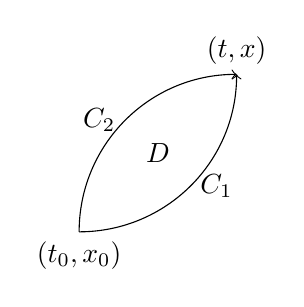
\begin{tikzpicture}
      \coordinate (A) at (0,0); %点Aの定義
      \coordinate (B) at (2,2); %点Bの定義
      \coordinate (M) at (1,1); %点Bの定義
      \draw (A) node[below] {$\qty(t_0,x_0)$}; %点A
      \draw (B) node[above] {$\qty(t,x)$}; %点B
      \draw[->] (A) to[out=0,in=-90] node[right]{$C_1$} (B);
      \draw[->] (A) to[out=90,in=180] node[left]{$C_2$} (B);
      \draw (M) node {$D$};
    \end{tikzpicture}
    上の図のようになるとき,平面領域に対するGreenの定理により,\begin{align*}
      \int\qty(P\dd{t}+Q\dd{x})=\iint_D\qty(-\pdv{P}{x}+\pdv{Q}{t})\dd{t}\dd{x}
    \end{align*}となる.可積分条件より\begin{align*}
      -\pdv{P}{x}+\pdv{Q}{t}=0
    \end{align*}なので,右辺は0.従って\begin{align*}
      \int_{C_1}\qty(P\dd{t}+Q\dd{x})=\int_{C_2}\qty(P\dd{t}+Q\dd{x})
    \end{align*}
    途中で交差しているときは,交差する前と後で分けて考えればよい.
  \end{proof}
\end{note}
\begin{example}
  \begin{align*}
    \redast:\qty(x\sin t-t)\dd{t}+\qty(x^2-\cos t)\dd{x}=0
  \end{align*}を解く.
  \begin{align*}
    \pdv{P}{x}=\sin t=\pdv{Q}{t}
  \end{align*}であるから,これは全微分型\\
  $\qty(t_0,x_0)=\qty(0,0)$と取って,\begin{align*}
    \varphi\qty(t,x)=\int_0^xQ\qty(0,y)\dd{y}+\int_0^tP\qty(s,x)\dd{s}
  \end{align*}とおくと,\begin{align*}
    \int_0^xQ\qty(0,y)\dd{y} & =\int_0^x\qty(y^2-1)\dd{y}=\qty[\frac{y^3}{3}-y]_0^x=\frac{x^3}{3}-x                                            \\
    \int_0^tP\qty(s,x)       & =\int_0^t\qty(x\sin s-s)\dd{s}=\qty[-x\cos s-\frac{s^2}{2}]_{s=0}^{s=t}=\qty(-x\cos t-\frac{t^2}{2})-\qty(-x-0)
  \end{align*}
  従って\begin{align*}
    \varphi\qty(t,x)=-x\cos t-\frac{t^2}{2}+\frac{x^3}{3}
  \end{align*}となる.\redast の一般解は\begin{align*}\varphi=\qty(\text{定数})
  \end{align*}より\begin{align*}
    -x\cos t-\frac{t^2}{2}+\frac{x^3}{3} & =C & \qty(C\text{は任意定数})
  \end{align*}
  \textbf{[別解]}\begin{align*}
    \pdv{\varphi}{t}=P=x\sin t-t
  \end{align*}の両辺を$x$は定数だと思って$t$について積分\begin{align*}
    \int\pdv{\varphi}{t}\dd{t} & =\int\qty(x\sin t-t)\dd{t}                                                                      \\
    \varphi\qty(t,x)           & =-x\cos t-\frac{t^2}{2}+C\qty(x) & \qty(x\text{は定数と思うので積分定数は}x\text{の関数でよい})
  \end{align*}
  この両辺を$x$で偏微分すると\begin{align*}
    \pdv{\varphi}{x}=-\cos t+C^\prime \qty(x)
  \end{align*}
  これが\begin{align*}
    \pdv{\varphi}{x}=Q=x^2-\cos t
  \end{align*}に一致する.すなわち\begin{align*}
                      & C^\prime \qty(x)=x^2     \\
    \Leftrightarrow\, & C\qty(x)=\frac{x^3}{3}+C
  \end{align*}
  従って\begin{align*}
    \varphi\qty(t,x)=-x\cos t-\frac{t^2}{2}+\qty(\frac{x^3}{3}+C)
  \end{align*}となって,解は\begin{align*}
    \varphi=\qty(\text{定数})
  \end{align*}より\begin{align*}
    -x\cos t-\frac{t^2}{2}+\frac{x^3}{3}=C_1
  \end{align*}と書ける.\\
  (\underline{注} \redast が全微分型でないときは,この計算はうまくいかない)
\end{example}
\subsection{全微分型でないとき}
\begin{align*}
  \redast : P+Q\dv{x}{t}=0
\end{align*}が全微分型でなくてもこの両辺にある関数$\mu\qty(t,x)$をかけると\begin{align*}
  \qty(\mu P)+\qty(\mu Q)\dv{x}{t}=0
\end{align*}が全微分型になることがある.このような$\mu=\mu\qty(t,x)$を\redast の\underline{積分因子}という.

一般には積分因子$\mu\qty(t,x)$を求めるのは難しいが,$\mu$が$t$のみの関数$\mu\qty(t)$,または$\mu$が$x$のみの関数$\mu\qty(x)$と仮定して積分因子が求まることがある.この場合を考える.

$\mu=\mu\qty(t)$に対して\begin{align*}
                    & \redast:\qty(\mu P)\dd{t}+\qty(\mu Q)\dd{x}=0 \text{が全微分型}                           \\
  \Leftrightarrow\, & \pdv{\qty(\mu P)}{x}=\pdv{\qty(\mu Q)}{t}                       & \qty(\text{可積分条件}) \\
  \Leftrightarrow\, & \mu\pdv{P}{x}=\dv{\mu}{t}Q+\mu\pdv{Q}{t}                                                  \\
  \Leftrightarrow\, & \mu\qty(\pdv{P}{x}-\pdv{Q}{t})=\dv{\mu}{t}Q
\end{align*}
このとき\begin{align*}
  \frac{\dv{\mu}{t}}{\mu}=\frac{\pdv{P}{x}-\pdv{Q}{t}}{Q}
\end{align*}で右辺は$t$のみの関数なので\begin{align*}
  f\qty(t)=\frac{\dv{\mu}{t}}{\mu}
\end{align*}とおくと,\begin{align*}
  \int\frac{\dv{\mu}{t}}{\mu}\dd{t} & =\int f\qty(t)\dd{t}     \\
  \int\frac{1}{\mu}\dd{u}           & =\int f\qty(t)\dd{t}     \\
  |\mu|                             & =e^{\int f\qty(t)\dd{t}}
\end{align*}となって\begin{align*}
  \mu=e^{\int f\qty(t)\dd{t}}
\end{align*}ととれる(積分定数は何でもよい).
\begin{summary}
  \begin{equation*}
    \redast:P\dd{t}+Q\dd{x}=0
  \end{equation*}において
  \begin{itemize}
    \item $\displaystyle\pdv{P}{x}-\pdv{Q}{t}=0$のとき,\redast は全微分型
    \item $\displaystyle\pdv{P}{x}-\pdv{Q}{t}\neq 0$のとき,
          \begin{itemize}
            \item $\displaystyle\frac{\pdv{P}{x}-\pdv{Q}{t}}{Q}$が$t$のみの関数$f\qty(t)$となるとき,$\displaystyle\mu\qty(t)=e^{\int f\qty(t)\dd{t}}$を積分因子にとれる.
            \item $\displaystyle\frac{\pdv{Q}{t}-\pdv{P}{x}}{P}$が$x$のみの関数$g\qty(x)$となるとき,$\displaystyle\mu\qty(x)=e^{\int g\qty(x)\dd{x}}$を積分因子にとれる.
          \end{itemize}
  \end{itemize}
\end{summary}
\begin{example}
  \begin{align*}
    \redast:e^x\dd{t}+\qty(-2t^2x-te^x)\dd{x}=0
  \end{align*}
  を考える.
  \begin{align*}
    \pdv{P}{x}=e^x\neq \pdv{Q}{t}=-4tx-e^x
  \end{align*}なので,\redast は全微分型でない.
  \begin{align*}
    \frac{\pdv{P}{x}-\pdv{Q}{t}}{Q}=\frac{e^x+4tx+e^x}{-2t^2x-te^x}=-\frac{2}{t}\ \qty(t\text{のみの関数})
  \end{align*}となるので,\begin{align*}
    \mu\qty(t)=e^{\int-\qty(\frac{2}{t})\dd{t}}=e^{\log t^{-2}}=t^{-2}
  \end{align*}が\redast の積分因子にとれる.\\
  \redast の両辺に$t^{-2}$をかけて\begin{align*}
    \reddast:t^{-2}e^x\dd{t}+t^{-2}\qty(-2t^2x-te^x)\dd{x}=0
  \end{align*}
  \begin{align*}
    \tilde{P} & =t^{-2}e^x                             \\
    \tilde{Q} & =t^{-2}\qty(-2t^2x-te^x)=-2x-t^{-1}e^x
  \end{align*}とおく.
  ここで\begin{align*}
    \qty(t_0,x_0)=\qty(1,0)
  \end{align*}ととって\,(注$t=0$では$t^{-2}$は定義されないので$t_0=1$とする.)\begin{align*}
    \varphi\qty(t,x)=\int_0^x \tilde{Q}\qty(1,y)\dd{y}+\int_1^t\tilde{P}\qty(s,x)\dd{s}
  \end{align*}とおくと,\begin{empheq}[left=\empheqlbrace]{align*}
    \int_0^x\tilde{Q}\qty(1,y)\dd{y}&=\int_0^x\qty(-2y-e^y)\dd{y}=\qty[-y^2-e^y]_{y=0}^{y=x}=\qty(-x^2-e^x)-\qty(0-1)\\
    \int_1^t\tilde{P}\qty(s,x)\dd{x}&=\int_1^ts^{-2}e^x\dd{s}=\qty[\frac{s^{-2+1}}{-2+1}e^x]_{s=1}^{s=t}=\qty(-\frac{1}{t}e^x)-\qty(-e^x)
  \end{empheq}
  \begin{align*}
    \varphi\qty(t,x)=-x^2-\frac{1}{t}e^x+1
  \end{align*}となるので,\reddast の一般解(すなわち\redast の一般解)は\begin{align*}
    \varphi=\qty(\text{定数})
  \end{align*}より\begin{align*}
    -\frac{1}{t}e^x-x^2-C
  \end{align*}となる.
\end{example}
\section{べき級数法}
「求積」で解けない場合の究極の方法

ODEの解を\begin{align*}
  x\qty(t) & =\sum_{n=0}^\infty a_n t^n & \qty(a_n\text{は定数})
\end{align*}と仮定して,これをもとのODEに代入して,係数$a_0,a_1,\ldots$を順に決めていく方法.
\begin{example}
  \begin{align*}
    \dv{x}{t}=tx
  \end{align*}の解$x\qty(t)$で\begin{align*}
    x\qty(0)=C\qty(\text{定数})
  \end{align*}を満たすものを求める.
  \begin{align*}
    x\qty(t)=a_0+a_1t+a_2t^2+a_3t^3+\cdots
  \end{align*}とおいてこれを$t$で微分.\begin{align*}
    \dv{x}{t}=a_1+2a_2t+3a_3t^2+\cdots=\sum_{n=1}^\infty na_nt^{n-1}=\sum_{n=0}^\infty\qty(n+1)a_{n+1}t^n
  \end{align*}
  一方\begin{align*}
    tx=t\qty(a_0+a_1t+a_2t^2+a_3t^3+\cdots)=a_0t+a_1t^2+a_2t^3+\cdots=\sum_{n=1}^\infty a_{n-1}t^n
  \end{align*}
  この両辺の$t^0,t^1,t^2,\ldots$の各係数を比較\begin{empheq}[left=\empheqlbrace]{align*}
    a_1&=0\\
    2a_2&=a_0\\
    &\vdots\\
    \qty(n+1)a_{n+1}&=a_{n-1}\\
    &\vdots
  \end{empheq}
  よって1つおきの漸化式\begin{align*}
    na_n=a_{n-2}
  \end{align*}となる.
  \begin{itemize}
    \item $n=2m+1$(奇数)のとき,$a_1=0,3a_3=a_1=0,\cdots$となって\begin{align*}
            a_n=0
          \end{align*}
    \item $n=2m$(偶数)のとき,\begin{align*}
            2ma_{2m} & =a_{2m-2}                                                                       \\
            a_{2m}   & =\frac{a_{2\qty(m-1)}}{2m}=\frac{1}{2m}\frac{a_{2\qty(m-2)}}{2\qty(m-1)}=\cdots \\
                     & =\frac{a_0}{2m\cdot 2\qty(m-1)\cdots 2}=\frac{C}{2^mm!}
          \end{align*}
          従って\begin{align*}
            x\qty(t)=\sum_{m=0}^\infty a_{2m}t^{2m}=C\qty(\sum_{m=0}^\infty\frac{1}{2^mm!}t^{2m})=C\sum_{m=0}^\infty\frac{\qty(\frac{t^2}{2})^m}{m!}=Ce^{\frac{t^2}{2}}
          \end{align*}となる.
  \end{itemize}
\end{example}
\section{線型常微分方程式系の一般的性質}
$n$個の未知関数$x_1\qty(t),\ldots,x_n\qty(t)$を\begin{align*}
  \va{x}\qty(t)=\mqty(
  x_1\qty(t) \\\vdots\\x_n\qty(t)
  )
\end{align*}とまとめて書く$\qty(\va{x}:\bbR\to\bbR)$.\begin{align*}
  \redast:\dv{\va{x}}{t}=A\qty(t)\va{x}\qty(t)+\va{r}\qty(t)
\end{align*}ただし,\begin{align*}
  A\qty(t)=\qty(a_{ij}\qty(t))
\end{align*}は各成分が連続関数となる$n\times n$行列で,\begin{align*}
  \dv{\va{x}}{t}=\mqty(
  \dv{x_1}{t} \\\vdots\\\dv{x_n}{t}
  ),\va{r}\qty(t)=\mqty(
  r_1\qty(t)  \\\vdots\\r_n\qty(t)
  ):\text{各成分が連続}
\end{align*}を考える(\underline{線型常微分方程式系}\,or\,\underline{連立線型ODE}という).\\
$\va{r}\qty(t)=\va{0}$のとき\underline{同次(or斉次)方程式}という.$\va{r}\qty(t)\neq\va{0}$のとき\underline{非同次(or非斉次)方程式}という.
\subsection{同次方程式と非同次方程式の関係}\begin{align*}
  \redo: & \dv{\va{x}}{t}=A\qty(t)\va{x}                                               \\
  \redn: & \dv{\va{x}}{t}=A\qty(t)\va{x}+\va{r}\qty(t) & \qty(\va{r}\qty(t)\neq\va{0})
\end{align*}とするとき
\begin{enumerate}
  \item $\va{x_p}\qty(t)$が\redn の1つの解(特解or特殊解という)で,$\va{x_o}\qty(t)$が\redo の任意の解のとき,$\va{x_o}+\va{x_p}$は\redn の解
        \begin{proof}
          \begin{align*}
            \dv{t}\qty(\va{x_o}+\va{x_p})=\dv{\va{x_0}}{t}+\dv{\va{x_p}}{t}=A\qty(t)\va{x_0}+\qty(A\qty(t)\va{x_p}+\va{r}\qty(t))=A\qty(t)\qty(\va{x_o}+\va{x_p})+\va{r}\qty(t)
          \end{align*}
        \end{proof}
  \item 逆に$\va{x_1}\qty(t),\va{x_2}\qty(t)$が\redn の任意の解$\Rightarrow\,\va{x_1}-\va{x_2}$は\redo の解
        \begin{proof}
          \begin{align*}
            \dv{t}\qty(\va{x_1}-\va{x_2})=\qty(A\qty(t)\va{x_1}+\va{r}\qty(t))-\qty(A\qty(t)\va{x_2}+\va{r}\qty(t))=A\qty(t)\qty(\va{x_1}-\va{x_2})
          \end{align*}
        \end{proof}
\end{enumerate}
\begin{note}
  1,2を合わせると\begin{align*}
    \qty{\redn \text{の解全体}}=\va{x_p}+\qty{\redo \text{の解全体}}
  \end{align*}となり$\qty{\redn\text{の解全体}}$は$\qty{\redo \text{の解全体}}$を$\va{x_p}$だけ平行移動したものとなる.(従って\redn の1つの解$\va{x_p}$と\redo の任意の解が求まれば,\redn の任意の解が求まる)
\end{note}
\subsection{解の存在と一意性}
\begin{align*}
  \redast:\dv{\va{x}}{t}=A\qty(t)\va{x}+\va{r}\qty(t)
\end{align*}の解$\va{x}\qty(t)$で任意の初期条件\begin{align*}
  \va{x}\qty(0)=\va{a}\qty(\in\bbR^n\qty(\text{or}\,\bbC^n))
\end{align*}を満たすものが\underline{ただ一つ存在する}
\subsection{同次方程式の解の重ね合わせ}
$\va{z}\qty(t),\va{w}\qty(t)$が\begin{align*}
  \redo:\dv{\va{x}}{t}=A\qty(t)\va{x}
\end{align*}の解で,かつ$k\in\bbR\qty(\text{or}\,\bbC)$とすると,$\va{z}+\va{w},k\va{z}$も\redo の解
\begin{proof}
  \begin{align*}
    \dv{\qty(\va{z}+\va{w})}{t} & =\dv{\va{z}}{t}+\dv{\va{w}}{t}=A\qty(t)\va{z}+A\qty(t)\va{w}=A\qty(t)\qty(\va{z}+\va{w}) \\
    \dv{\qty(k\va{z})}{t}       & =k\dv{\va{z}}{t}=kA\qty(t)\va{z}=A\qty(t)\qty(k\va{z})
  \end{align*}
\end{proof}
\noindent[意味]:$\qty{\redo の解全体}$は和とスカラー倍に関して閉じていて\underline{ベクトル空間をなす}(1つの解$\qty(\va{x}\qty(t))_{t\in\bbR}$を1本のベクトルと思う)
\subsection{同次方程式の解空間}
\begin{align*}
  \redo:\dv{\va{x}}{t}=A\qty(t)\va{x}
\end{align*}に対する解の存在と一意性により
\begin{align*}
  \begin{array}{ccc}
    \qty{\redo \text{の解全体}}    & \stackrel{F}{\longrightarrow} & \bbR^n\qty(\text{or}\,\bbC^n) \\
    \rotatebox{90}{$\in$}          &                               & \rotatebox{90}{$\in$}         \\
    \qty(\va{x}\qty(t))_{t\in\bbR} & \longmapsto                   & \va{x}\qty(t)
  \end{array}
\end{align*}
この$F$は線形写像$\qty(F\qty(\va{z}+\va{w})=F\qty(\va{z})+F\qty(\va{w}),F\qty(k\va{z})=kF\qty(\va{z}))$なので,この$F$により\begin{align*}
  \qty{\redo \text{の解全体}\qty(\text{原点}\va{x}\qty(t)=\va{0}\text{を通る})} & \cong\bbR^n\qty(\text{or}\,\bbC^n) & \qty(\text{ベクトル空間として同型}\qty(\text{同じとみなせる}))
\end{align*}
従って\begin{align*}
  \va{r}\qty(t)\neq\va{0}
\end{align*}に対して$\qty{\redn \text{の解全体}}$は$\bbR^n$を特解$\va{x_p}$の分だけ平行移動したものとなる.

\underline{$n=2$}のとき

\begin{tikzpicture}
  \draw (-3,0)--(-2,1);
  \draw (-2,1)--(2,0);
  \draw (2,0)--(1,-1);
  \draw (1,-1)--(-3,0);

  \draw (-2,2)--(-1,3);
  \draw (-1,3)--(3,2);
  \draw (3,2)--(2,1);
  \draw (2,1)--(-2,2);

  \draw[->] (-0.5,0)--(0.5,2);

  \draw (-0.5,0)node[left]{O};
  \draw (0, 1)node[right]{$\va{x_p}$};

  \draw (1.5, -0.5)node[right]{\{\redo の解全体\}};
  \draw (2.5, 1.5)node[right]{\{\redn の解全体\}};
\end{tikzpicture}
\section{$n$階線型ODE}
関数$y=y\qty(t)$に対する\begin{align*}
  \reddast & :y^{\qty(n)}+P_{n-1}\qty(t)y^{\qty(n-1)}+\cdots+P_1\qty(t)y^\prime +P_0\qty(t)y=Q\qty(t) & \qty(\text{各}P_i\qty(t),Q\qty(t)\text{は与えられた関数},y^{\qty(k)}=\dv[k]{y}{t})
\end{align*}は\begin{align*}
  \va{x}\qty(t)=\mqty(
  y\qty(t)         \\
  y^\prime \qty(t) \\
  \vdots           \\
  y^{\qty(n-1)}\qty(t)
  )\end{align*}とおくと\begin{align*}
  \reddast\Leftrightarrow\dv{\va{x}}{t}\qty(=\mqty(
  y^\prime                                                                                                           \\
  y^{\prime\prime}                                                                                                   \\
  \vdots                                                                                                             \\
    y^{\qty(n)}
  ))          & =\mqty(
  y^\prime                                                                                                           \\
  y^{\prime\prime}                                                                                                   \\
  \vdots                                                                                                             \\
  y^{\qty(n-1)}                                                                                                      \\
  -P_{n-1}\qty(t)y^{\qty(n-1)}-\cdots-P_1\qty(t)y^\prime -P_0\qty(t)y+Q\qty(t)
  )           & \qty(y^{\qty(n)}\text{が}\reddast \text{により規定されると見る})                                     \\
              & =\mqty(
  0           & 1                                                                &        &        &                 \\
              & \ddots                                                           & \ddots &        & \Largezero      \\
  \Largezero  &                                                                  & \ddots & \ddots &                 \\
              &                                                                  &        & \ddots & 1               \\
  -P_0\qty(t) &                                                                  &        &        & -P_{n-1}\qty(t)
  )\mqty(
  y                                                                                                                  \\y^\prime \\\vdots\\\vdots\\y^{\qty(n-1)}
  )+\mqty(
  0                                                                                                                  \\\vdots\\\vdots\\0\\Q\qty(t)
  )
\end{align*}となり,$A\qty(t)=\mqty(
  0                  & 1      &        &        &                        \\
  & \ddots & \ddots &        & \Largezero             \\
  \Largezero         &        & \ddots & \ddots &                        \\
  &        &        & \ddots & 1                      \\
  -P_0\qty(t) &        &        &        & -P_{n-1}\qty(t)
  ),\va{x}\qty(t)=\mqty(
  y \\y^\prime \\\vdots\\\vdots\\y^{\qty(n-1)}
  ),\va{r}=\mqty(
  0 \\\vdots\\\vdots\\0\\Q\qty(t)
  )$とおくと,\redast に帰着できる.従って\begin{align*}
  \redo: & y^{\qty(n)}+P_{n-1}\qty(t)y^{\qty(n-1)}+\cdots+P_1\qty(t)y^\prime +P_0\qty(t)y=0                               \\
         & y^{\qty(n)}+P_{n-1}\qty(t)y^{\qty(n-1)}+\cdots+P_1\qty(t)y^\prime +P_0\qty(t)y=Q\qty(t) & \qty(Q\qty(t)\neq 0)
\end{align*}に対して先と同様のことが成り立ち,
\begin{itemize}
  \item $\qty{\text{同次方程式}\redo \text{の解全体}}$は$n$次元ベクトル空間をなし,解$y\qty(t)$は初期値\begin{align*}\va{x}\qty(0)=\mqty(
          y\qty(0)         \\
          y^\prime \qty(0) \\
          \vdots           \\
          y^{\qty(n)}\qty(0)
          )\in\bbR^n\qty(\text{or}\,\bbC^n)\end{align*}を与えるごとにただ1つ定まる.
  \item $\qty{\text{非同次方程式}\redn\text{の解}}$は\redn の特解$y_p\qty(t)$が1つ求まると$y_p+\qty{\redo \text{の解全体}}$と書ける.
\end{itemize}
\underline{Question} \ \redo の$n$個の解はいつ1次独立となるか?(いつ\redo の解空間の基底をなすか)
\section{関数の1次独立性の判定}
一般に$X_1\qty(t),\ldots,X_n\qty(t)$が$C^\infty$級関数のとき\begin{align*}
                                          & X_1,\ldots,X_n\text{が}\qty(\text{関数として})\text{\underline{1次独立}}                                                  \\
  \stackrel{\text{定義}}{\Leftrightarrow} & \text{定数}C_1,\ldots C_n\text{に対して「}C_1X_1+\cdots C_nX_n\equiv 0\Rightarrow C_1=0,\cdots,C_n=0\text{」が成り立つ.}
\end{align*}
ここで$\equiv$は関数として(すべての$t$で)0の意.
\begin{align*}C_1X_1+\cdots +C_nX_n\equiv 0\end{align*}の両辺を$k$回微分すると\begin{align*}C_1X_1^{\qty(k)}+\cdots C_nX_n^{\qty(k)}=0\end{align*}これを$k=0,1,\ldots,n-1$についてまとめると\begin{align*}\mqty(
  X_1             & \cdots & X_n             \\
  X_1^\prime      & \cdots & X_n^\prime      \\
  \vdots          &        & \vdots          \\
  X_1^{\qty(n-1)} & \cdots & X_n^{\qty(n-1)}
  )\mqty(
  C_1                                        \\\vdots\\\vdots\\C_n
  )\equiv\va{0}\end{align*}となる.ここで$n\times n$行列$X\qty(t)$を\begin{align*}X\qty(t)=\mqty(
  X_1             & \cdots & X_n             \\
  X_1^\prime      & \cdots & X_n^\prime      \\
  \vdots          &        & \vdots          \\
  X_1^{\qty(n-1)} & \cdots & X_n^{\qty(n-1)}
  )\end{align*}とおく.ここでもしある$t=t_0$で\begin{align*}\det(X\qty(t_0))\not\equiv 0\end{align*}となれば$X\qty(t_0)^{-1}$が存在するのでこれを\begin{align*}X\qty(t_0)\mqty(
  C_1 \\\vdots\\C_n
  )=\va{0}\end{align*}の両辺にかけて\begin{align*}\mqty(
  C_1 \\\vdots\\C_n
  )=\va{0}\end{align*}を得る.従ってこのとき$X_1\qty(t),\ldots,X_n\qty(t)$は(関数として) 1次独立となる.
\begin{conclusion}
  $n$個の関数$X_1\qty(t),\ldots,X_n\qty(t)$に対してある$t=t_0$で\begin{align*}\mdet{
    X_1\qty(t_0)             & \cdots & X_n\qty(t_0)             \\
    X_1^\prime \qty(t_0)     & \cdots & X_n^\prime \qty(t_0)     \\
    \vdots                   &        & \vdots                   \\
    X_1^{\qty(n-1)}\qty(t_0) & \cdots & X_n^{\qty(n-1)}\qty(t_0)
    }\not\equiv\va{0}\,\Rightarrow\, X_1\qty(t),\ldots,X_n\qty(t)\text{は1次独立}\end{align*}
  $\mdet{
    X_1\qty(t_0)                    & \cdots & X_n\qty(t_0)                    \\
    X_1^\prime \qty(t_0)                   & \cdots & X_n^\prime \qty(t_0)                   \\
    \vdots                                 &        & \vdots                                 \\
    X_1^{\qty(n-1)}\qty(t_0) & \cdots & X_n^{\qty(n-1)}\qty(t_0)
    }$を$X_1,\ldots,X_n$の$t=t_0$でのWronskian(ロンスキアン)といい$W\qty[X_1,\ldots,X_n]\qty(t)$と書く.
\end{conclusion}
\begin{example}
  \begin{align*}X_1\qty(t)=e^{\lambda_1t},\cdots,X_n\qty(t)=e^{\lambda_nt}\text{で}\lambda_1,\ldots,\lambda_n\text{が\underline{相異なる定数}}\Rightarrow\,X_1,\ldots,X_n\text{は1次独立}\end{align*}
  \begin{proof}
    \begin{align*}X_j\qty(t)=e^{\lambda_jt}\end{align*}に対して\begin{align*}
      X_j^{\qty(k)}\qty(t) & =\lambda_j^ke^{\lambda_jt} \\
      X_j^{\qty(k)}\qty(0) & =\lambda_j^k
    \end{align*}となるので\begin{align*}
      W\qty[X_1,\ldots,X_n]\qty(0)=\mdet{
      1               & \cdots & 1               \\
      \lambda_1       & \cdots & \lambda_n       \\
      \lambda_1^2     & \cdots & \lambda_n^2     \\
      \vdots          &        & \vdots          \\
      \lambda_1^{n-1} & \cdots & \lambda_n^{n-1}
      }\,\qty(=\Lambda \text{とおく})
    \end{align*}
    このとき,\underline{主張}\begin{align*}
      \lambda_1,\ldots,\lambda_n\text{が相異なる} & \Rightarrow\,\Lambda=0 & \qty(\text{従って}X_1,\ldots,X_n\text{は1次独立})
    \end{align*}
    \begin{proof}
      $\Lambda$で$\lambda_i=\lambda_j$とすると(i列)=(j列)となって$\Lambda=0$となる.したがって因数定理により$\Lambda$は$\qty(\lambda_j=\lambda_i)\,\qty(j\neq i)$を因数に持ち$\prod_{1\leq i\leq j\leq n}\qty(\lambda_j-\lambda_i)$で割り切れる.ところで\begin{align*}
        \qty(\Lambda の次数)=0+1+\cdots+n-1                                             & =\frac{n\qty(n-1)}{2} & \qty(\det \text{は各行から1個ずつ選ぶ}) \\
        \qty(\prod_{1\leq i\leq j\leq n}\qty(\lambda_j-\lambda_i)の次数)=_n\mathrm{C}_2 & =\frac{n\qty(n-1)}{2}
      \end{align*}
      で同じなので\begin{align*}\Lambda=\qty(\text{定数})\prod_{1\leq i\leq j\leq n}\qty(\lambda_j-\lambda_i)\end{align*}となる.ここで「添え字の大きなものができるだけ多くかかる項」を見ると\begin{align*}
        \Lambda \text{では}\mdet{
        1                                                                                       &           &        &                 \\
                                                                                                & \lambda_2 &        &                 \\
                                                                                                &           & \ddots &                 \\
                                                                                                &           &        & \lambda_n^{n-1}
        }\text{の取り方で}\det\text{での係数}                                                   & =1                                   \\
        \prod_{1\leq i\leq j\leq n}\qty(\lambda_j-\lambda_i)では\lambda_j \text{の方なので係数} & =1
      \end{align*}従って(定数)=1.今\begin{align*}i\neq j\Rightarrow\lambda_j-\lambda_i\neq 0\end{align*}なので\begin{align*}\Lambda=\prod_{1\leq i\leq j\leq n}\qty(\lambda_j-\lambda_i)\neq 0\end{align*}となる.
    \end{proof}
  \end{proof}
\end{example}
\begin{supple}(関数の1次独立性の判定)
  \begin{example}
    自然数$n$に対して$X_1\qty(t)=1,X_2\qty(t)=t,\cdots,X_n\qty(t)=t^{n-1}$は1次独立
    \begin{proof}
      \begin{align*}
        \text{Wronskian}\,W\qty[X_1,\ldots,X_n]\qty(t) & =\mdet{
        X_1                                            & \cdots     & X_n                                                            \\
        X_1^\prime                                     & \cdots     & X_n^\prime                                                     \\
        \vdots                                         &            & \vdots                                                         \\
        X_1^{\qty(n-1)}                                & \cdots     & X_n^{\qty(n-1)}
        }                                                                                                                            \\
                                                       & =\mdet{
        1                                              & t          & t^2             & \cdots & t^{n-1}                             \\
        0                                              & 1          & 2t              & \cdots & \qty(n-1)t^{n-2}                    \\
        0                                              & 0          & 2               & \ddots & \vdots                              \\
        \vdots                                         & \vdots     & \vdots          & \ddots & \vdots                              \\
        0                                              & 0          & 0               & \cdots & \qty(n-1)!
        }                                                                                                                            \\
                                                       & =\mdet{
        1                                              &            &                 &        &                  &                  \\
                                                       & 1          &                 &        &                  & \text{\Large{*}} \\
                                                       &            & 2               &        &                  &                  \\
                                                       &            &                 & 3!     &                  &                  \\
                                                       & \Largezero &                 &        & \ddots           &                  \\
                                                       &            &                 &        &                  & \qty(n-1)!
        }                                                                                                                            \\
                                                       & =\mdet{
        0!                                             &            &                 &        &                                     \\
                                                       & 1!         &                 &        & \text{\Large{*}}                    \\
                                                       &            & 2!              &        &                                     \\
                                                       & \Largezero &                 & \ddots &                                     \\
                                                       &            &                 &        & \qty(n-1)!
        }=0!\times 1!\times\cdots\times\qty(n-1)!\neq 0
      \end{align*}
      なので$X_1\qty(t),\ldots X_n\qty(t)$は1次独立
    \end{proof}
  \end{example}
  \begin{example}
    定数$\lambda$に対して$Y_1\qty(t)=e^{\lambda t},Y_2\qty(t)=te^{\lambda t},\cdots,Y_n\qty(t)=t^{n-1}e^{\lambda t}$は1次独立.
    \begin{proof}
      もし$Y_1,\ldots,Y_n$が1次従属とすると\begin{align*}C_1Y_1\qty(t)+\cdots+C_nY_n\qty(t)\equiv 0\end{align*}となる定数\begin{align*}\qty(C_1,\ldots,C_n)\neq\qty(0,\cdots,0)\end{align*}がとれる.この式の両辺に$e^{-\lambda t}\qty(\neq 0)$をかけると\begin{align*}C_1\cdot 1+C_2\cdot t+\cdots+C_nt^{n-1}\equiv 0\end{align*}となる定数\begin{align*}\qty(C_1,\ldots,C_n)\neq\qty(0,\cdots,0)\end{align*}が存在して,これは前の例に矛盾.したがって$Y_1,\ldots Y_n$は1次独立
    \end{proof}
  \end{example}
\end{supple}
\section{定数係数$n$階同次線型ODE}
未知関数$x=x\qty(t)$に対する\begin{align*}
  \redo: & x^{\qty(n)}+a_{n-1}x^{n-1}+\cdots+a_1x^\prime +a_0x=0 & \qty(a_0,\ldots,a_{n-1}\text{は定数})
\end{align*}の$n$個の1次独立な解(\redo の解空間$\qty(\cong\bbR^n)$の基底)を求めたい.

\underline{記号} : $x$から$x^\prime =\dv{x}{t}$を作る操作を$D$で表す(微分作用素).\begin{align*}
  Dx=x^\prime ,D^2x=D\qty(Dx)=x^{\prime\prime} ,\cdots,D^nx=x^{\qty(n)}
\end{align*}
すると\redo は\begin{align*}\qty(D^n+a_{n-1}D^{n-1}+\cdots+a_1D+a_0)x=0\end{align*}と書ける.$D^n+a_{n-1}D^{n-1}+\cdots+a_1D+a_0$を$P\qty(D)$($D$の$n$次式)とおく.次に,$\qty(D^n+a_{n-1}D^{n-1}+\cdots+a_1D+a_0)$の中で$D$を未知数$\lambda$に代えて\begin{align*}P\qty(\lambda)=\lambda^n+a_{n-1}\lambda^{n-1}+\cdots+a_1\lambda+a_0=0\end{align*}という$n$次方程式(\redo の\underline{特性方程式}という)を考える($P\qty(\lambda)$を\redo の\underline{特性多項式}という).ここで\begin{align*}
  P\qty(\lambda) & =\qty(\lambda-\lambda_1)^{m_1}\cdots\qty(\lambda-\lambda_r)^{m_r} & \qty(\lambda_1,\ldots,\lambda_r\text{は相異なり}m_1+\cdots+m_r=n)
\end{align*}と因数分解できたとする.すると\redo は\begin{align*}\qty(D-\lambda_1)^{m_1}\cdots\qty(D-\lambda_r)^{m_r}x=0\end{align*}となる.
\begin{note}
  定数$\lambda$に対して\begin{align*}\qty(\lambda x)^\prime =\lambda x^\prime \end{align*}即ち\begin{align*}D\qty(\lambda x)=\lambda Dx\end{align*}となるので\begin{align*}D\lambda=\lambda D\end{align*}となって$D$と定数倍は順番を代えてよい(\underline{可換}という).これにより$\qty(D-\lambda_1)^{m_1}\cdots\qty(D-\lambda_r)^{m_r}$を展開すると$D^n+a_{n-1}D^{n-1}+\cdots+a_1D+a_0$になる.一方,$D$と関数$f\qty(t)$倍は可換でない.実際\begin{align*}D\qty(f\qty(t)x\qty(t))=f^\prime \qty(t)x\qty(t)+f\qty(t)x^\prime \qty(t)=\qty(Df)x+fDx\end{align*}となって$\qty(Df)x$の分だけずれる.
\end{note}
このとき$i\neq j$に対して\begin{align*}\qty(D-\lambda_i)^{m_i}\qty(D-\lambda_j)^{m_j}=\qty(D-\lambda_j)^{m_j}\qty(D-\lambda_i)^{m_i}\end{align*}となるので$\qty(D-\lambda_i)^{m_i}$を1番先に$x$に作用させて,各$i=1,\ldots,r$に対して\begin{align*}\qty(D-\lambda_i)^{m_i}x=0\end{align*}を考えると,これの$m_i$個の1次独立な解として$e^{\lambda_0 t},te^{\lambda_1 t},\ldots,t^{m_i-1}e^{\lambda_i t}$が得られる.
\begin{proof}
  添え字$i$を略して$t^ke^{\lambda t}\,\qty(l=0,\ldots,m-1)$が\begin{align*}\qty(D-\lambda)^mx=0\end{align*}の1次独立な解を言う.$x$が\begin{align*}\qty(D-\lambda)^mx=0\end{align*}を満たすとして\begin{align*}y\qty(t)=e^{-\lambda t}x\end{align*}とおくと\begin{align*}
    Dy     & =\qty(e^{-\lambda t}x)^\prime =\qty(e^{-\lambda t})^\prime x+e^{-\lambda t}x^\prime =\qty(-\lambda e^{-\lambda t})x+e^{-\lambda t}Dx=e^{-\lambda t}\qty(D-\lambda)x                                                 \\
    D^2y   & =D\qty(e^{-\lambda t}\qty(D-\lambda)x)=\qty(e^{-\lambda t})^\prime \qty(D-\lambda)x+e^{-\lambda t}D\qty(D-\lambda)x=e^{-\lambda t}\qty(D-\lambda)^2x                                                                \\
    \vdots &                                                                                                                                                                                                                     \\
    D^my   & =e^{-\lambda t}\qty(D-\lambda)^mx=0                                                                                                                                 & \qty(\qty(D-\lambda)^mx=0\,\qty(\text{仮定}))
  \end{align*}となるので,$y$は$1,t,\ldots,t^{n-1}$の1次結合で書ける.\begin{align*}x=e^{\lambda t}y\end{align*}なので$x$は$e^{\lambda t},te^{\lambda t},\ldots,t^{n-1}e^{\lambda t}$の1次結合で書ける.
\end{proof}
従って\redo の$n\qty(=m_1+\cdots+m_r)$個の解として$\qty{t^ke^{\lambda_j t}\,\qty(k=0,\ldots,m_j-1.j=1,\ldots,r)}$が得られる.\\
\underline{主張}\,これらは全体として\underline{1次独立}になる(従って\redo の解空間の基底になる)
\begin{proof}
  これらの1次結合で0になったとする.\begin{equation}
    \sum_{j=1}^r\qty{\sum_{k=0}^{m_j-1}c_{j,k}t^ke^{\lambda_jt}}=0\label{star}\tag{*}
  \end{equation}
  このとき各$c_{j,k}=0$を言えばよい.
  \begin{itemize}
    \item[Case 1] 各$j=1,\ldots,r$に対して\begin{align*}\sum_{k=0}^{m_j-1}c_{j,k}t^ke^{\lambda_jt}=0\end{align*}とすると$\qty{e^{\lambda_jt},te^{\lambda_jt},\ldots,t^{m_j-1}e^{\lambda_jt}}$が1次独立であったので各$c_{j,k}=0$となってOK.
    \item[Case 2] ある$j_0$に対して\begin{align*}\sum_{k=0}^{m_{j_0}-1}c_{j_0,k}t^ke^{\lambda_{j_0}t}\neq 0\end{align*}とする.このときは\begin{align*}x_j\qty(t)=\sum_{k=0}^{m_j-1}c_{j,k}t^ke^{\lambda_{j_0}t}\end{align*}とおいて次を言えばよい.\\
          \underline{主張2}\ $x_j\qty(t)\,\qty(j=1,\ldots,r)$が\begin{align*}\qty(D-\lambda_j)^{m_j}x_j=0\end{align*}を満たし,そのうちの$j=1,\ldots,l$に対して\begin{align*}x_j\qty(t)\neq 0\end{align*}とするとき$x_j\qty(t)\,\qty(j=1,\ldots,l)$は1次独立.
          これが言えると,$x_{j_0}\neq 0$が\ref{star}により\begin{align*}x_{j_0}\qty(t)=\sum_{j\neq j_0}x_j\qty(t)\end{align*}と書けて主張2に反する.従って,Case 2は生じない.
          \begin{proof}
            主張2を示す.$x_1\qty(t),\ldots,x_l\qty(t)$が1次従属とすると,ある$x_{j_0}\qty(t)$が\begin{align*}x_{j_0}\qty(t)=\sum_{j=j_0}C_j\cdot x_j\qty(t)\end{align*}と書ける.ここで特性多項式\begin{align*}P\qty(\lambda)=\qty(\lambda-\lambda_1)^{m_1}\cdots\qty(\lambda-\lambda_r)^{m_r}\end{align*}の逆数を考えて,これを部分分数に分解すると,\begin{align*}\frac{1}{P\qty(\lambda)}=\frac{1}{\qty(\lambda-\lambda_1)^{m_1}\cdots\qty(\lambda-\lambda_r)^{m_r}}=\sum_{j=1}^r\frac{q_j\qty(\lambda)}{\qty(\lambda-\lambda_j)^{m_j}}\end{align*}と書ける($q_j\qty(\lambda)$は$\lambda$の$m_j-1$次式).この両辺に$P\qty(\lambda)$をかけると\begin{align*}1=\sum_{j=1}^rq_j\qty(\lambda)\qty(\lambda-\lambda_1)^{m_1}\cdots\qty(\lambda-\lambda_j)^{m_j}\cdots\qty(\lambda-\lambda_r)^{m_r}\end{align*}
            となる.ここで\begin{align*}\hat{P_j}\qty(\lambda)=\qty(\lambda-\lambda_1)^{m_1}\cdots\qty(\lambda-\lambda_j)^{m_j}\cdots\qty(\lambda-\lambda_r)^{m_r}\end{align*}とおく.すると\begin{align*}1=\sum_{j\neq j_0}q_j\qty(\lambda)\hat{P_j}\qty(\lambda)+q_{j_0}\qty(\lambda)\hat{P_{j_0}}\qty(\lambda)\end{align*}という$\lambda$の多項式になり,$\lambda$に$D$を代入して\begin{align*}
              I & =\sum_{j\neq j_0}q_j\qty(D)\hat{P_j}\qty(D)+q_{j_0}\qty(D)\hat{P_{j_0}}\qty(D) & \qty(I\text{は恒等写像})
            \end{align*}を得る.これを$x_{j_0}\qty(t)$に作用させると\begin{align*}
              Ix_{j_0}\qty(t) & =\sum_{j\neq j_0}q_j\qty(D)\hat{P_j}\qty(D)x_{j_0}\qty(t)+q_{j_0}\qty(D)\hat{P_{j_0}}\qty(D)x_{j_0}\qty(t)
            \end{align*}
            これの左辺は\begin{align*}Ix_{j_0}\qty(t)=x_{j_0}\qty(t)\neq 0\end{align*}
            一方右辺について,第1項は中に$\qty(D-\lambda_{j_0})^{m_{j_0}}$があるので0になる.第2項は$\hat{P_{j_0}}\qty(D)$の中に$\qty(D-\lambda_j)^{m_j}$があるので0になる.よって右辺は0となって矛盾.従って主張2が言えた.
          \end{proof}
  \end{itemize}
\end{proof}
\begin{conclusion}
  \begin{align*}\redo:x^{\qty(n)}+a_{n_1}x^{\qty(n-1)}+\cdots+a_1x^\prime +a_0x\qty(=\qty(D^n+a_{n-1}D^{n-1}+\cdots+a_1D+a_0)x)=0\end{align*}のすべての解は\redo を\begin{align*}\qty(D-\lambda_1)^{m_1}\cdots\qty(D-\lambda_r)^{m_r}x=0\end{align*}と書きなおすと\begin{align*}x\qty(t)=\sum_{j=1}^r\qty(\sum_{k=1}^{m_j-1}c_{j,k}t^ke^{\lambda_it})\end{align*}で与えられる($t^ke^{\lambda_it}$は1次独立).
\end{conclusion}
\begin{example}
  $\lambda_j$が複素数\begin{align*}\lambda_j=p+iq\,\qty(p,q\in\bbR)\end{align*}のときはEulerの公式\begin{align*}e^{i\theta}=\cos\theta+i\sin\theta\end{align*}を使うと\begin{align*}e^{\lambda_jt}=e^{\qty(p+iq)t}=e^{pt}e^{iqt}=e^{pt}\qty(\cos\qty(qt)+i\sin\qty(qt))\end{align*}と書ける.このまま全て$\bbC$上で考えて任意定数$C_{j,k}\in\bbC$としてもよいが,$a_0,\ldots,a_{n-1}\in\bbR$のときは,$\lambda_j$と$\bar{\lambda_j}=p-iq$が同時にpairとして現れ,同じ重複度を持つので,\begin{align*}
    e^{\lambda_jt}       & =e^{pt}\qty(\cos\qty(qt)+i\sin\qty(qt)) \\
    e^{\bar{\lambda_j}t} & =e^{pt}\qty(\cos\qty(qt)-i\sin\qty(qt))
  \end{align*}が同時に現れる.ここで\begin{align*}
    \frac{1}{2}\qty(e^{\lambda_jt}+e^{\bar{\lambda_j}t})  & =e^{pt}\cos\qty(qt) \\
    \frac{1}{2i}\qty(e^{\lambda_jt}-e^{\bar{\lambda_j}t}) & =e^{pt}\sin\qty(qt)
  \end{align*}
  となり,逆に$e^{\lambda_jt}$と$e^{\bar{\lambda_j}t}$はこの2つの1次結合で書ける.従って,$t^ke^{\lambda_jt}$を$t^ke^{pt}\cos\qty(qt)$に,$t^ke^{\bar{\lambda_jt}t}$を$t^ke^{pt}\sin\qty(qt)$に代えても1次独立性は不変(どちらも\begin{align*}\qty(D-\lambda_j)^{m_j}\qty(D-\bar{\lambda_j})^{m_j}x=0\end{align*}の解空間の基底をなす→実数値関数としての\redo の解空間の基底を作れる).
\end{example}
\begin{example}
  \begin{align*}
    \redo:x^{\prime\prime} +3x^\prime +2=0
  \end{align*}のとき,\begin{align*}
    x^{\prime\prime} +3x^\prime +2=\qty(D^2+3D+2)x
  \end{align*}
  特性方程式は\begin{align*}
    \lambda^2+3\lambda+2=\qty(\lambda+1)\qty(\lambda+2)=0
  \end{align*}その解は\begin{align*}
    \lambda=-1,2
  \end{align*}より,$e^{\qty(-1)t},e^{\qty(-2)t}$を作る.\redo の一般解(全ての解)は\begin{align*}
    x\qty(t) & =C_1e^{-t}+C_2e^{-2t} & \qty(C_1,C_2\text{は任意定数})
  \end{align*}
\end{example}
\begin{example}
  \begin{align*}
    \redo:\qty(D^4-5D^3+9D^2-7D+2)x=0
  \end{align*}のとき,特性方程式は\begin{align*}
    \lambda^4-5\lambda^3+9\lambda^2-7\lambda+2 & =\qty(\lambda-2)\qty(\lambda-1)^3=0
  \end{align*}その解は\begin{align*}
    \lambda=1\,\qty(\text{重複度}3),\lambda=2
  \end{align*}より,$e^{1t},te^{1t},t^2e^{1t},e^{2t}$を作る.\redo の一般解は\begin{align*}x\qty(t)=C_1e^t+C_2te^t+C_3t^2e^t+C_4e^{2t}\end{align*}
\end{example}
\begin{example}
  \begin{align*}\redo:\qty(D^2+D+1)x=0\end{align*}の一般解を実数値関数で表す.
  \begin{align*}
    \lambda^2+\lambda+1=\qty(\lambda+\frac{1}{2})^2+\frac{3}{4}=0
  \end{align*}より\begin{align*}\lambda=\frac{-1\pm\sqrt{3}i}{2}\end{align*}より,$e^{\frac{-1\pm\sqrt{3}i}{2}t}=e^{-\frac{t}{2}}e^{\pm\frac{\sqrt{3}}{2}it}$を作る.$e^{\pm\frac{\sqrt{3}}{2}it}$は$\cos\qty(\frac{\sqrt{3}}{2}t),\sin\qty(\frac{\sqrt{3}}{2}t)$に代える.
  \begin{align*}x\qty(t)=C_1e^{-\frac{t}{2}}\cos\qty(\frac{\sqrt{3}}{2}t)+C_2e^{-\frac{t}{2}}\sin\qty(\frac{\sqrt{3}}{2}t)\end{align*}
\end{example}
\begin{example}
  \begin{align*}\redo:D^3\qty(D^2+1)^2x=0\end{align*}のとき
  \begin{align*}
    \lambda^3\qty(\lambda^2+1)^2=\lambda^3\qty(\qty(\lambda-i)\qty(\lambda+i))^2=0
  \end{align*}の解は\begin{align*}\lambda=0\qty(\text{重複度}3),\pm i\qty(\text{重複度}2)\end{align*}より,$e^{0t},te^{0t},t^2e^{0t},e^{\pm it},te^{\pm it}$を作り,$e^{\pm it},te^{\pm it}$を$\cos t,\sin t$に代える.\redo の一般解は\begin{align*}x\qty(t)=C_1+C_2t+C_3t^2+C_4\cos t+C_5\sin t+C_6t\cos t+C_7t\sin t\end{align*}
\end{example}
\section{定数係数非同次線型ODE(未定係数法)}
\underline{目標}:未知関数$x=x\left(t\right)$に対する\begin{align*}
  \redast:x^{\qty(n)}+a_{n-1}x^{\qty(n-1)}+\cdots+a_1x^\prime +a_0x=Q\qty(t)
\end{align*}
$D=\dv{t}$として\begin{align*}
  \qty(D^n+a_{n-1}D^{n-1}+\cdots+a_1D+a_0)x=Q\qty(t)
\end{align*}ここで$a_0,\ldots,a_{n-1}$は定数.$Q\qty(t)$は$t^me^{at}$($m$は0以上の整数,$a$は定数)たちの1次結合で$Q\qty(t)\neq 0$\\
の一般解を求めたい.

\noindent [解き方]
\begin{itemize}
  \item[Step 1] \redast の両辺に(右辺)の\underline{$Q\qty(t)$を消す微分作用素$E$}をかける.\begin{example}
          $Q\qty(t)=t^me^{at}$のときは\begin{align*}
            E=\qty(D-a)^{m+1}
          \end{align*}$Q\qty(t)=t^m\cos\qty(bt)\qq{or}t^m\sin\qty(bt)$のときは\begin{align*}
            E=\qty(D^2+b^2)^{m+1}
          \end{align*}ととればよい.
        \end{example}
  \item[Step 2] すると,同次方程式\begin{align*}
          \reddast:E\qty(D^n+a_{n-1}D^{n-1}+\cdots+a_1D+a_0)x=0
        \end{align*}を得る\,(\underline{注}\,\redast の解$\Rightarrow$\reddast の解).この\reddast の一般解を求め,それをもとの\redast に代入して\redast を満たすように任意定数を特定すると\redast の一般解を得る($Q\qty(t)$が和の形のときはその各々について上のことを行えばよい).
\end{itemize}
\begin{example}
  \begin{align*}
    \redast:\qty(D^2+3D+2)x=e^t
  \end{align*}のとき,(右辺)の$e^t$は\begin{align*}
    \qty(D-1)e^t=\qty(e^t)^\prime -e^t=0
  \end{align*}を満たすので,\redast の両辺に$\qty(D-1)$をかけると\begin{align*}
    \reddast:\qty(D-1)\qty(D^2+3D+2)x=0
  \end{align*}
  \reddast の一般解:\reddast の特性方程式\begin{align*}
    \qty(\lambda-1)\qty(\lambda^2+3\lambda+2)=0
  \end{align*}の解は$\lambda=1,-1,-2$より,$e^{1t},e^{\qty(-1)t},e^{-2t}$を作る.\reddast の一般解は\begin{align*}
    x\qty(t)=C_1e^t+C_2e^{-t}+C_3e^{-2t}
  \end{align*}これを元の\redast に代入.このうち$C_2e^{-t}+C_3e^{-2t}$の分は\begin{align*}
    \qty(D^2+3D+2)x=0
  \end{align*}を満たすものなので\redast に代入すると0になる.そこで$x\qty(t)=C_1e^t$を\redast に代入して任意定数$C_1$を特定する:\begin{align*}
    \qty(D^2+3D+2)C_1e^t=C_1\qty(\qty(e^t)^{\prime\prime} +3\qty(e^t)^\prime +2e^t)=C_1\qty(1+3+2)e^t=6C_1e^tx
  \end{align*}で,これが\redast の(右辺)の$e^t$に一致\,$\Leftrightarrow\,6C_1=1\,\Leftrightarrow C_1=\frac{1}{6}$.従って\redast の一般解は\begin{align*}
    x\qty(t)=\frac{1}{6}e^t+C_2^{-t}+C_3e^{-2t}
  \end{align*}
\end{example}
\begin{example}
  \begin{align*}
    \redast:\qty(D^3+1)x=t^2
  \end{align*}のとき,(右辺)の$t^2$は\begin{align*}
    D^3\qty(t^2)=0
  \end{align*}を満たすので\redast の両辺に$D^3$をかけると\begin{align*}
    \reddast:D^3\qty(D^3+1)x=0
  \end{align*}になる.\\
  \reddast の一般解:特性方程式\begin{align*}
    \lambda^3\qty(\lambda^3+1)=\qty(\lambda+1)\qty(\qty(\lambda-\frac{1}{2})^2+\frac{3}{4})=0
  \end{align*}の解は$\lambda=0\qty(\text{重複度}3),-1,\frac{1}{2}\pm\frac{\sqrt{3}}{2}i$より,$e^{0t},te^{0t},t^2e^{0t},e^{\qty(-1)t},e^{\qty(\frac{1}{2}\pm\frac{\sqrt{3}}{2}i)t}=e^\frac{1}{2}e^{\pm i\frac{\sqrt{3}}{2}}$を作り,$e^{\pm i\frac{\sqrt{3}}{2}t}$を$\cos\qty(\frac{\sqrt{3}}{2}t),\sin\qty(\frac{\sqrt{3}}{2}t)$に代える.\reddast の一般解は\begin{align*}
    x\qty(t)=C_1+C_2t+C_3t^2+C_4e^{-t}+C_5e^{\frac{t}{2}}\cos\qty(\frac{\sqrt{3}}{2}t)+C_6e^{\frac{t}{2}}\sin\qty(\frac{\sqrt{3}}{2}t)
  \end{align*}
  $C_4e^{-t}+C_5e^{\frac{t}{2}}\cos\qty(\frac{\sqrt{3}}{2}t)+C_6e^{\frac{t}{2}}\sin\qty(\frac{\sqrt{3}}{2}t)$は$\qty(D^3+1)x=0$を満たす分なので\redast に代入すると0になる.そこで\begin{align*}
    x\qty(t)=C_1+C_2t+C_3t^2
  \end{align*}を元の\redast に代入:\begin{align*}
    \qty(D^3+1)\qty(C_1+C_2t+C_3t^2)=0+\qty(C_1+C_2t+C_3t^2)
  \end{align*}で,これが\redast の(右辺)の$t^2$に一致\,$\Leftrightarrow$\,$C_1=0,C_2=0,C_3=1$.したがって\redast の一般解は\begin{align*}
    x\qty(t)=t^2+C_4e^{-t}+C_5e^{\frac{t}{2}}\cos\qty(\frac{\sqrt{3}}{2}t)+C_6e^{\frac{t}{2}}\sin\qty(\frac{\sqrt{3}}{2}t)
  \end{align*}
\end{example}
\begin{example}
  \begin{align*}
    \redast:\qty(D+1)\qty(D+3)x=e^{-t}
  \end{align*}のとき\begin{align*}
    \qty(D+1)e^{-t}=0
  \end{align*}なので\redast の両辺に$\qty(D+1)$をかけると\begin{align*}
    \reddast:\qty(D+1)^2\qty(D+3)x=0
  \end{align*}になる.\reddast の特性方程式\begin{align*}
    \qty(\lambda+1)^2\qty(\lambda+3)=0
  \end{align*}の解は$\lambda=-1\qty(\text{重複度}2),-3$より,$e^{\qty(-1)t},te^{\qty(-1)t},e^{-3t}$を作る.\reddast の一般解は\begin{align*}
    x\qty(t)=C_1e^{-t}+C_2te^{-t}+C_3e^{-3t}
  \end{align*}$C_1e^{-t}+C_3e^{-3t}$は\begin{align*}
    \qty(D+1)\qty(D+3)x=0
  \end{align*}を満たす分なので\redast に代入すると0になる.そこで\begin{align*}
    x\qty(t)=C_2te^t
  \end{align*}を元の\redast に代入して$C_2$を特定する:\begin{align*}
    \qty(D+1)\qty(D+3)C_2te^{-t} & =\qty(D+3)\qty(D+1)C_2te^{-t}=\qty(D+3)C_2e^{-t}                      \\
                                 & =C_2\qty(\qty(e^{-t})^\prime +3e^{-t})=C_2\qty(-1+3)e^{-t}=2C_2e^{-t}
  \end{align*}これが\redast の右辺の$e^{-t}$に一致\,$\Leftrightarrow\,2C_2=2\,\Leftrightarrow\,C_2=\frac{1}{2}$.従って\redast に一般解は\begin{align*}
    x\qty(t)=C_1e^{-t}+\frac{1}{2}te^{-t}+C_3e^{-3t}
  \end{align*}
\end{example}
\begin{example}
  \begin{align*}
    \redast:\qty(D^2-1)x=t\sin t
  \end{align*}
  (右辺)の$t\sin t$は\begin{align*}
    \qty(D^2+1)^2\qty(t\sin t)=\qty(D^2+1)\qty(D^2+1)\qty(t\sin t)=\qty(D^2+1)2\cos t=0
  \end{align*}を満たすので\redast の両辺に$\qty(D^2+1)^2$を書けると\begin{align*}
    \reddast:\qty(D^2+1)^2\qty(D^2-1)x=0
  \end{align*}になる.\reddast の特性方程式\begin{align*}
    \qty(\lambda^2+1)^2\qty(\lambda^2-1)=\qty(\qty(\lambda-i)\qty(\lambda+i))^2\qty(\lambda+1)\qty(\lambda-1)=0
  \end{align*}の解は$\lambda=\pm i\qty(\text{重複度}2),-1,1$より,$e^{\pm it},te^{\pm it},e^{\qty(-1)t},e^{1t}$を作り,$e^{\pm it},te^{\pm it}$を$\cos t,\sin t$に代える.\reddast の一般解は\begin{align*}
    x\qty(t)=C_1\cos t+C_2\sin t+C_3t\cos t+C_4t\sin t+C_5e^t+C_6e^{-t}
  \end{align*}$C_5e^t+C_6e^{-t}$を\redast に代入すると0になる.そこで$C_1\cos t+C_2\sin t+C_3t\cos t+C_4t\sin t$を\redast に代入して$C_1\sim C_4$を特定する.$\cos t$は$\qty(D^2+1)$をかけると0になるので\redast の(左辺)の$\qty(D^2+1)-2$と書くと\begin{align*}
      & \qty(D^2-1)\qty(C_1\cos t+C_2\sin t+C_3t\cos t+C_4t\sin t)                                                                                          \\
    = & \qty(D^2+1)\qty(C_1\cos t+C_2\sin t)-2\qty(C_1\cos t+C_2\sin t)+\qty(D^2+1)\qty(C_3t\cos t+C_4t\sin t)-2\qty(C_3t\cos t+C_4t\sin t)                 \\
    = & 0-2\qty(C_1\cos t+C_2\sin t)+\qty(C_3\qty(\cos t-t\sin t)+C_4\qty(\sin t-t\cos t))^\prime +\qty(C_3t\cos t+C_4t\sin t)-2\qty(C_3t\cos t+C_4t\sin t) \\
    = & \qty(-2C_1+2C_4)\cos t+\qty(-2C_2-2C_3)\sin t+\qty(-2C_3)t\cos t+\qty(-2C_4)t\sin t
  \end{align*}これが\redast の(右辺)の$t\sin t$に一致
  \begin{empheq}[left=\Leftrightarrow\empheqlbrace]{align*}
    -2C_1+2C_4&=0\\
    -2C_2-2C_3&=0\\
    -2C_3&=0\\
    -2C_4&=1
  \end{empheq}
  \begin{empheq}[left=\Leftrightarrow\empheqlbrace]{align*}
    C_1&=-\frac{1}{2}\\
    C_2&=0\\
    C_3&=0\\
    C_4&=-\frac{1}{2}
  \end{empheq}
  \redast の一般解は\begin{align*}
    x\qty(t)=-\frac{1}{2}\cos t-\frac{1}{2}t\sin t+C_5e^t+C_6e^{-t}
  \end{align*}
\end{example}
\section{$n$階非同次線型ODEに対する定数変化法}
\noindent \underline{目標}\,未知関数$x=x\qty(t)$に対する\begin{align*}
  \redo & :x^{\qty(n)}+P_{n-1}\qty(t)x^{\qty(n-1)}+\cdots+P_1\qty(t)x^\prime +P_0\qty(t)x=0 & \qty(P_0,\ldots,P_{n-1}\text{は与えられた関数})
\end{align*}の$n$個の解$\varphi_1\qty(t),\ldots,\varphi_n\qty(t)$でそのWronskian\begin{align*}
  W\qty[\varphi_1,\ldots,\varphi_n]\qty(t)=\mdet{\varphi_1 & \cdots & \varphi_n                    \\
  \varphi_1^\prime                                         & \cdots & \varphi_n^\prime             \\
  \vdots                                                   &        & \vdots                       \\
  \varphi_1^{\qty(n-1)}                                    & \cdots & \varphi_n^{\qty(n-1)}}\neq 0
\end{align*}となるもの(従って$\qty{\varphi_1,\ldots,\varphi_n}$は1次独立となり\redo の解空間$\qty(\cong\bbR^n)$の基底をなす)が分かったとする.このとき$Q\qty(t)\neq 0$に対する非同次方程式\begin{align*}
  \redast & :x^{\qty(n)}+P_{n-1}\qty(t)x^{\qty(n-1)}+\cdots+P_1\qty(t)x^\prime +P_0\qty(t)x=Q\qty(t) & \qty(Q\qty(t)\text{与えられた関数})
\end{align*}の一般解を求めたい.\\
方針: \redo の一般解\begin{align*}
  x\qty(t) & =\sum_{i=1}^{n}C_i\varphi_i\qty(t) & \qty(C_1,\ldots,C_n\text{は任意定数})
\end{align*}において$C_i$を関数$C_i\qty(t)$に代えて(定数を変化させて)\begin{align*}
  x\qty(t)=\sum_{i=1}^{n}C_i\qty(t)\varphi_i\qty(t)
\end{align*}が\redast を満たすように$C_1\qty(t),\ldots,C_n\qty(t)$を決めたい.\begin{align*}
  x^\prime =\sum_i\qty(C_i\varphi_i)^\prime =\sum_iC_i^\prime \varphi_i+\sum_iC_i\varphi_i^\prime
\end{align*}
ここで(このままでは任意性が大きすぎるので)$C_i\,\qty(i=1,\ldots,n)$に\begin{align*}
  \sum_iC_i^\prime \varphi_i=0
\end{align*}という条件を課す.すると\begin{align*}
  x^\prime =\sum_iC_i\varphi_i^\prime
\end{align*}となり
\begin{align*}
  x^{\prime\prime} =\sum_i\qty(C_i\varphi_i^\prime )=\sum_iC_i^\prime \varphi_i^\prime +\sum_iC_i\varphi_i^{\prime\prime}
\end{align*}となる.ここでさらに\begin{align*}
  \sum_iC_i^\prime \varphi_i^\prime =0
\end{align*}という条件を課す.すると\begin{align*}
  x^{\prime\prime} =\sum_iC_i\varphi_i^{\prime\prime}
\end{align*}となる.(以下同様)\\
$x^{\qty(n-1)}$において
\begin{align*}
  \sum_iC_i^\prime \varphi_i^{\qty(n-2)}=0
\end{align*}という条件を課すと\begin{align*}
  x^{\qty(n-1)}=\sum_iC_i\varphi_i^{\qty(n-1)}
\end{align*}となる.すると\begin{align*}
  x^{\qty(n)}=\sum_iC_i^\prime \varphi_i^{\qty(n-1)}+\sum_iC_i\varphi_i^{\qty(n)}
\end{align*}となり,このとき\begin{align*}
    & x^{\qty(n)}+P_{n-1}\qty(t)x^{\qty(n-1)}+\cdots+P_1\qty(t)x^\prime +P_0\qty(t)x                                                                                                                                          \\
  = & \sum_iC_i\varphi_i^{\qty(n-1)}+\sum_iC_i\qty(\varphi^{\qty(n)}+P_{n_1}\qty(t)\varphi_i^{\qty(n-1)}+\cdots+P_1\qty(t)\varphi_i^\prime +P_0\qty(t)\varphi_i)
  = & \sum_iC_i^\prime \varphi_i^{\qty(n-1)}                                                                                                                     & \qty(\varphi_1,\ldots,\varphi_n\text{は}\redo \text{の解})
\end{align*}となるので,これが\redast の右辺の$Q\qty(t)$になればよい.\\
$C_1,\ldots,C_n$に課される条件をまとめると
\begin{empheq}[left=\empheqlbrace]{align*}
  \sum_iC_i^\prime \varphi_i&=0\\
  \sum_iC_i^\prime \varphi_i^\prime &=0\\
  \vdots&\\
  \sum_iC_i^\prime \varphi_i^{\qty(n-2)}&=0\\
  \sum_iC_i^\prime \varphi_i^{\qty(n-1)}&=Q\qty(t)
\end{empheq}
即ち,
\begin{align*}
  \mqty(\varphi_1       & \cdots & \varphi_n             \\
  \varphi_1^\prime      & \cdots & \varphi_n^\prime      \\
  \vdots                &        & \vdots                \\
  \varphi_1^{\qty(n-2)} & \cdots & \varphi_n^{\qty(n-2)} \\
  \varphi_1^{\qty(n-1)} & \cdots & \varphi_n^{\qty(n-1)}
  )\mqty(
  c_1^\prime                                             \\\vdots\\\vdots\\\vdots\\c_n^\prime
  )=\mqty(
  0                                                      \\\vdots\\0\\0\\Q\qty(t)
  )
\end{align*}となる.従って\begin{align*}
  \mqty(
  c_1^\prime                                             \\\vdots\\\vdots\\c_n^\prime
  )=\mqty(\varphi_1     & \cdots & \varphi_n             \\
  \varphi_1^\prime      & \cdots & \varphi_n^\prime      \\
  \vdots                &        & \vdots                \\
  \varphi_1^{\qty(n-1)} & \cdots & \varphi_n^{\qty(n-1)}
  )^{-1}\mqty(
  0                                                      \\\vdots\\0\\Q\qty(t)
  )
\end{align*}が求まり,この各成分を積分すると$C_1\qty(t),\ldots,C_n\qty(t)$が求まる.
\begin{note}
  $\sum_iC_i^\prime \varphi_i=0,\sum_iC_i^\prime \varphi_i^\prime =0$の条件を課さないといけない,という必然性はないが,こうすることで$C_1\qty(t),\ldots,C_n\qty(t)$がうまく求まるというのが定数変化法(しかもこの方法をより一般の連立線型ODEの場合にも拡張できる).
\end{note}
Cramerの公式($n\times n$行列$A=\qty(a_{ij})$の$\det A\neq 0$のとき連立1次方程式$A\va{x}=\va{b}$の解$\va{x}=\mqty(x_1\\\vdots\\x_n)$が\begin{align*}
  x_j=\frac{1}{\det A}\mdet{
    \cline{3-3}
  a_{11} & \cdots & \multicolumn{1}{|c|}{ }      & \cdots & a_{n1} \\
  \vdots & \cdots & \multicolumn{1}{|c|}{\va{b}} & \cdots & \vdots \\
  a_{1n} & \cdots & \multicolumn{1}{|c|}{ }      & \cdots & a_{nn} \\
    \cline{3-3}
  }
\end{align*}で与えられる.)を使うと\begin{align*}
  C_j\qty(t)=\int\frac{1}{W\qty[\varphi_1,\ldots,\varphi_n]\qty(t)}\mdet{
    \cline{3-3}
  \varphi_1             &        & \multicolumn{1}{|c|}{0}        &        & \varphi_n             \\
  \varphi_1^\prime      &        & \multicolumn{1}{|c|}{\vdots}   &        & \varphi_n^\prime      \\
  \vdots                & \cdots & \multicolumn{1}{|c|}{0}        & \cdots & \vdots                \\
  \varphi_1^{\qty(n-1)} &        & \multicolumn{1}{|c|}{Q\qty(t)} &        & \varphi_n^{\qty(n-1)} \\
    \cline{3-3}
  }\dd{t}
\end{align*}とも書ける.
\begin{example}
  \begin{align*}
    \redast:\qty(D^2+1)x=\frac{1}{\cos t}
  \end{align*}のとき\begin{align*}
    \redo:\qty(D^2+1)x=0
  \end{align*}の一般解は\begin{align*}
    x\qty(t)=C_1\cos t+C_2\sin t
  \end{align*}$\varphi_1\qty(t)=\cos t,\varphi_2\qty(t)=\sin t$とおく.ここで$C_i$を$C_i\qty(t)$に代えて\begin{align*}
    x\qty(t)=\sum_{i=1}^2C_i\qty(t)\varphi_i\qty(t)
  \end{align*}が\redast を満たすように$C_1\qty(t),C_2\qty(t)$を決めたい.そのためには
  \[\mqty(C_1^\prime  \\C_2^\prime )=\mqty(
    \varphi_1  & \varphi_2  \\
    \varphi_1^\prime & \varphi_2^\prime
    )^{-1}\mqty(0     \\\frac{1}{\cos t})\]
  を満たせばよい.
  \begin{align*}
    \mqty(C_1^\prime  \\C_2^\prime )=\mqty(
    \cos t  & \sin t  \\
    -\sin t & \cos t
    )^{-1}\mqty(0     \\\frac{1}{\cos t})=\mqty(
    \cos t  & -\sin t \\
    \sin t  & \cos t
    )\mqty(0          \\\frac{1}{\cos t})=\mqty(\frac{-\sin t}{\cos t}\\0)
  \end{align*}この各成分を積分:
  \begin{empheq}[left=\empheqlbrace]{align*}
    C_1\qty(t)&=\int\frac{-\sin t}{\cos t}\dd{t}=\log\mdet{\cos t}+C_1&\qty(C_1\text{は任意定数})\\
    C_2\qty(t)&=\int 1\dd{t}=t+C_2&\qty(C_2\text{は任意定数})
  \end{empheq}
  従って\redast の一般解は\begin{align*}
    x\qty(t) & =\qty(\log\abs{\cos t}+C_1)\cos t+\qty(t+C_2)\sin t             \\
             & =\qty(\log\abs{\cos t})\cos t+t\sin t+\qty(C_1\cos t+C_2\sin t)
  \end{align*}
\end{example}
\underline{Qustion}\begin{align*}
  \redo:x^{\qty(n)}+P_{n-1}\qty(t)x^{\qty(n-1)}+\cdots+P_1\qty(t)x^\prime +P_0\qty(t)x=0
\end{align*}の$n$個の1次独立な解$\varphi_1\qty(t),\ldots,\varphi_n\qty(n)$が求まるのはどういうときか?\
\begin{itemize}
  \item $n=1$のときは1階線型なのでOK
  \item 一般の$n$でも\underline{定数係数}$\qty(P_i\qty(t)=a_i\qty(\text{定数}))$となるときは\redo の特性方程式\begin{align*}
          \lambda^n+a_{n-1}\lambda^{n-1}+\cdots+a_1\lambda+a_0=0
        \end{align*}が解ければOK
  \item しかし,一般の場合には\redo の解空間の基底$\varphi_1\qty(t),\ldots,\varphi_n\qty(n)$を求めるような一般的な方法はない.
\end{itemize}
定数係数の場合に帰着できるものとして
\subsection{Euler型ODE}
未知関数$x=x\qty(t)$
\[t^nx^{\qty(n)}+b_{n-1}t^{n-1}x^{\qty(n-1)}+\cdots+b_1tx^\prime+b_0x=0\ \qty(b_0,\ldots,b_{n-1}\text{は与えられた関数,即ち}P_i\qty(t)=t^{-n}\qty(b_it^i))\]
\subparagraph{[解き方]}
$t=e^s$とおいて変数を$t$から$s$に変換する\,:
\[\dv{t}{s}=\dv{e^s}{s}=e^s=t\]
なので
\[\dv{x}{s}=\dv{x}{t}\dv{t}{s}=t\dv{x}{t}=\qty(t\cdot\dv{t})x\]
となって
\[t\dv{t}=\dv{s}\]
と書ける.
\begin{align*}
  \dv[2]{x}{s}
   & =\dv{s}\qty(\dv{x}{s})                 \\
   & =\dv{s}\qty(\dv{s}x)                   \\
   & =\qty(t\dv{t})\qty(t\dv{t}x)           \\
   & =t\qty(\dv{t}{t}\dv{x}{t}+t\dv[2]{t}x) \\
   & =t\dv{x}{t}+t^2+\dv[2]{x}{t}
\end{align*}
となるので
\[t^2\dv[2]{t}=\dv[2]{s}\dv{s}\]
\begin{align*}
  \dv[3]{x}{s}
   & =\qty(t\dv{t})\qty(t\dv{x}{t}+t^2\dv[2]{x}{t})                             \\
   & =t\qty(\qty(\dv{t}{t}+t\dv[2]{x}{t})+\qty(2t\dv[2]{x}{t}+t^2\dv[3]{x}{t})) \\
   & =t\dv{x}{t}+3t^2\dv[2]{x}{t}+t^3\dv[3]{x}{t}
\end{align*}
となるので,
\[t^3\dv[3]{t}=\dv[3]{s}-3\dv[2]{s}+2\dv{s}\]
以下同様にすると一般に
\[t^k\dv[k]{t}=\dv[k]{s}+\qty(\dv{s},\ldots,\dv[k-1]{s}\text{の定数係数の1次結合})\]
となるので
\[\redo:\qty(t^n\dv[n]{t}+b_{n-1}t^{n-1}\dv[n-1]{t}+\cdots+b_1t\dv{t}+b_0)x=0\]
を$x=x\qty(s)$に対する\underline{定数係数}の$n$階同次線型ODEに直せる.特に$n=2$のとき
\[t^2\dv[2]{x}{t}+b_1t\dv{x}{t}+b_0x=0\,\Leftrightarrow\,\qty(\dv[2]{s}-\dv{s})x+b_1\dv{s}x+b_0x=0\]
即ち,
\[\qty(\dv[2]{s}+\qty(b_1-1)\dv{s}+b_0)x\qty(s)=0\]
となる.
\begin{example}
  \[\redo:t^2x^{\prime\prime}+tx^{\prime}+4x=0\ \qty(b_1=1,b_0=4)\]
  のとき,\\
  $t=e^s$とおくと,
  \[\redo\,\Leftrightarrow\,\qty(\dv[2]{s}+\qty(1-1)\dv{s}+4)x\qty(s)=0\]
  即ち
  \[\dv[2]{x}{s}+4x=0\]
  となり,これの特性方程式は$\lambda^2+4=0$で,その解は$\lambda=\pm 2i$.$e^{\pm 2is}=e^{\pm i\qty(2s)}$を作り$\cos\qty(2s),\sin\qty(2s)$に代える.\redo の一般解は
  \[x\qty(s)=C_1\cos\qty(2s)+C_2\sin\qty(2s)\]
  ここで$t=e^s$より$s=\log t$.これは
  \[x\qty(t)=C_1\cos\qty(2\log t)+C_2\sin\qty(2\log t)\]
  と書ける.
  \[\redast:t^2x^{\prime\prime}+tx^{\prime}4x=1\]
  を定数変化法で解く.\redo の一般解
  \[x\qty(s)=C_1\cos\qty(2s)+C_2\sin\qty(2s)\]
  において$C_i$を$C_i\qty(s)$に代えて
  \[x\qty(s)=C_1\qty(s)\cos\qty(2s)+C_2\qty(s)\sin\qty(2s)\]
  の形で\redast を満たすように$C_1\qty(s),C_2\qty(s)$を求める($\varphi_1\qty(s)=\cos\qty(2s),\varphi_2\qty(s)=\sin\qty(2s)$とおく).そのためには
  \[\mqty(
    C_1^{\prime} \\
    C_2^{\prime}
    )=\mqty(
    \varphi_1 & \varphi_2 \\
    \varphi_1^{\prime} & \varphi_2^{\prime}
    )^{-1}\mqty(
    0 \\
    1
    )=\mqty(
    \cos\qty(2s) & -\frac{1}{2}\sin\qty(2s) \\
    \sin\qty(2s) & \frac{1}{2}\cos\qty(2s)
    )\mqty(
    0 \\
    1
    )\]
  を満たせばよい.これより
  \begin{align*}
    C_1^{\prime} & =-\frac{1}{2}\sin\qty(2s) \\
    C_2^{\prime} & =\frac{1}{2}\cos\qty(2s)
  \end{align*}
  と求まり,これらを$s$で積分して
  \begin{align*}
    C_1\qty(s) & =\int\qty(-\frac{1}{2}\sin\qty(2s))\dd{s}=\frac{1}{4}\cos\qty(2s)+C_1 \\
    C_2\qty(s) & =\int\frac{1}{2}\cos\qty(2s)\dd{s}=\frac{1}{4}\sin\qty(2s)+C_2
  \end{align*}
  従って\redast の一般解は
  \begin{align*}
    x\qty(s)
     & =\qty(\frac{1}{4}\cos\qty(2s)+C_1)\cos\qty(2s)+\qty(\frac{1}{4}\sin\qty(2s)+C_2)\sin\qty(2s) \\
     & =\frac{1}{4}+C_1\cos\qty(2s)+C_2\sin\qty(2s)
  \end{align*}
  $t$の関数として書くと
  \[x\qty(t)=\frac{1}{4}+C_1\cos\qty(2\log t)+C_2\sin\qty(2\log t)\]
\end{example}
\section{定数変化法(一般の連立線型ODEの場合)}
\subparagraph{復習}
未知関数$x=x\qty(t)$に対する$n$階非同次線型ODE
\[\redast:x^{\qty(n)}+P_{n-1}\qty(t)x^{\qty(n-1)}+\cdots+P_1\qty(t)x^\prime +P_0\qty(t)x=Q\qty(t)\quad\qty(P_0,\ldots,P_{n-1},Q\text{は与えられた関数,}Q\qty(t)\neq 0)\]
に対しては,
\[x^{\qty(n)}+P_{n-1}\qty(t)x^{\qty(n-1)}+\cdots+P_1\qty(t)x^\prime +P_0\qty(t)x=0\quad\qty(\text{同次方程式})\]
の$n$個の解$\varphi_1\qty(t),\ldots,\varphi_n\qty(t)$で
\[W\qty[\varphi_1,\ldots,\varphi_n]\qty(t)=\mdet{\varphi_1 & \cdots & \varphi_n                    \\
    \varphi_1^\prime                                         & \cdots & \varphi_n^\prime             \\
    \vdots                                                   &        & \vdots                       \\
    \varphi_1^{\qty(n-1)}                                    & \cdots & \varphi_n^{\qty(n-1)}}\neq 0\]
となるものが求まれば,\redast の一般解として
\[x\qty(t)=\sum_{i=1}^nC_i\qty(t)\varphi_i\qty(t)\]
で$C_1\qty(t),\ldots,C_n\qty(t)$が
\[\mqty(
  C_1^\prime\\
  \vdots\\
  C_n^\prime
  )=\mqty(
  \varphi_1&\cdots&\varphi_n\\
  \varphi_1^\prime&\cdots&\varphi_n^\prime\\
  \vdots&&\vdots\\
  \varphi_1^{\qty(n-1)}&\cdots&\varphi_n^{\qty(n-1)}
  )^{-1}\mqty(
  0\\
  \vdots\\
  0\\
  Q\qty(t)
  )\]
を満たすものとして与えられた.これを連立ODEとして書き直す.\[\va{x}\qty(t)=\mqty(
  x\qty(t)\\
  x^\prime\qty(t)\\
  \vdots\\
  x^{\qty(n-1)}\qty(t)
  ),A\qty(t)=\mqty(
  0&1&&&\Largezero\\
  &\ddots&\ddots&&\\
  &&\ddots&\ddots&\\
  \Largezero&&&0&1\\
  -P_0\qty(t)&\cdots&\cdots&\cdots&-P_{n-1}\qty(t)
  ),\va{b}\qty(t)=\mqty(
  0\\
  \vdots\\
  0\\
  Q\qty(t)
  )\]とおいて\redast と\redo を
\[\redast:\dv{\va{x}}{t}=A\qty(t)\va{x}+\va{b}\qty(t),\redo:\dv{\va{x}}{t}=A\qty(t)\va{x}\]
と各々書き直すと,\redo の$n$個の1次独立な解として$\va{v_i}\qty(t)=\mqty(
  \varphi_i\qty(t)\\
  \varphi_i^\prime\qty(t)\\
  \vdots\\
  \varphi_i^{\qty(n-1)}\qty(t)
  )\quad\qty(i=1,\ldots,n)$で
\[\det\qty(\va{v_1}\qty(t),\cdots,\va{v_n}\qty(t))\neq 0\]
となるものが得られ,\redast の一般解は
\[\va{x}\qty(t)=\mqty(
  \va{v_1}\qty(t)&\cdots&\va{v_n}\qty(t)
  )\mqty(
  C_1\qty(t)\\
  \vdots\\
  C_n\qty(t)
  )\]
と書け,$V\qty(t)=\mqty(
  \va{v_1}\qty(t)&\cdots&\va{v_n}\qty(t)
  )$とおくと,$\mqty(
  C_1\\
  \vdots\\
  C_n
  )$は
\[\mqty(
  C_1^\prime\\
  \vdots\\
  C_n^\prime
  )=V\qty(t)^{-1}\va{b}\qty(t)\]
を積分したものとして
\[\mqty(
  C_1\qty(t)\\
  \vdots\\
  C_n\qty(t)
  )=\int^t V\qty(s)^{-1}\va{b}\qty(s)\dd{s}\quad\qty(\text{不定積分})\]
と求まり,
\[\va{x}\qty(t)=V\qty(t)\mqty(
  C_1\qty(t)\\
  \vdots\\
  C_n\qty(t)
  )=\int^t V\qty(t)V\qty(s)^{-1}\va{b}\qty(s)\dd{s}\]
と書けることになる(不定積分に現れる任意定数は初期値$\va{x}\qty(t)$が与えられると定まる.)\\
この定式化を\underline{一般の連立線型ODE}にも拡張するため,まず$\va{v_i}\qty(t)=\mqty(
  \varphi_i\qty(t)\\
  \varphi_i^\prime\qty(t)\\
  \vdots\\
  \varphi_i^{\qty(n-1)}\qty(t)
  )$と$V\qty(t)=\mqty(
  \va{v_1}\qty(t)&\cdots&\va{v_n}\qty(t)
  )$と$V\qty(t)V\qty(s)^{-1}$を一般の場合に定式化する.
\section{基本行列と解核行列}
未知関数$\va{x}\qty(t)=\mqty(
  x_1\qty(t)\\
  \vdots\\
  x_n\qty(t)
  )$に対する同次線型ODE
\[\redo:\dv{\va{x}}{t}=A\qty(t)\va{x}\qty(t)\quad\qty(A\qty(t)=\qty(a_{ij}\qty(t))\text{は各成分}a_{ij}\qty(t)\text{が連続関数の}n\times n\text{行列})\]
をまず考える.\redo の$n$個の解$\va{v_1}\qty(t),\ldots,\va{v_n}\qty(t)$を横に並べて$V\qty(t)=\mqty(
  \va{v_1}\qty(t)&\cdots&\va{v_n}\qty(t)
  )\quad\qty(n\times n\text{行列})$と書き,ここで\underline{仮定$\det\qty(V\qty(t))\neq 0$}を満たすとする.(すると$\qty{\va{v_1},\ldots,\va{v_n}}$は\redo の解空間$\qty(\simeq\bbR^n)$の基底をなす)このとき
\[\dv{V}{t}=\mqty(
  \dv{\va{v_1}}{t}&\cdots&\dv{\va{v_n}}{t}
  )=\mqty(
  A\qty(t)\va{v_1}&\cdots&A\qty(t)\va{v_n}
  )=A\qty(t)\mqty(
  \va{v_1}&\cdots&\va{v_n}
  )=A\qty(t)V\qty(t)\]
となる.逆に$n\times n$行列$V\qty(t)$が$\dv{V}{t}=A\qty(t)V\qty(t)$を満たし$\det\qty(V\qty(t))\neq 0$のとき$V\qty(t)$を$\mqty(
  \va{v_1}\qty(t)&\cdots&\va{v_n}\qty(t)
  )$と書き,上の計算を逆にたどると,この$\va{v_1}\qty(t),\ldots,\va{v_n}\qty(t)$は\redo の$n$個の1次独立な解となる.そこで
\begin{dfn*}
  各成分が$C_1$級の$n\times n$行列$V\qty(t)=\qty(v_{ij}\qty(t))=\mqty(
    \va{v_1}\qty(t)&\cdots&\va{v_n}\qty(t)
    )$で$\dv{V}{t}=A\qty(t)V\qty(t),\det\qty(V\qty(t))\neq 0$を満たすものを\redo の\underline{基本行列}という.
\end{dfn*}
$X\qty(t)=\mqty(\va{x_1}\qty(t)&\cdots&\va{x_n}\qty(t)),Y\qty(t)=\mqty(\va{y_1}\qty(t)&\cdots&\va{y_n}\qty(t))$が共に\redo の基本行列のとき$\va{x_1}\qty(t),\cdots,\va{x_n}\qty(t)$は\redo の解空間の基底をなすので各$\va{y_k}\qty(t)\quad\qty(k=1,\ldots,n)$はこれらの1次結合として
\[\va{y_k}\qty(t)=\sum_{j=1}^n C_{jk}\va{x_j}\qty(k)=\mqty(
  \va{x_1}\qty(t)&\cdots&\va{x_n}\qty(t)
  )\mqty(
  C_{1k}\\
  \vdots\\
  C_{nk}
  )\quad\qty(\text{各}C_{jk}\text{は定数})\]
と書け,
\[Y\qty(t)=\mqty(\va{y_1}\qty(t)&\cdots&\va{y_n}\qty(t))=\mqty(
  \va{x_1}\qty(t)&\cdots&\va{x_n}\qty(t)
  )\mqty(
  C_{11}&\cdots&C_{1n}\\
  \vdots&&\vdots\\
  C_{n1}&\cdots&C_{nn}
  )=X\qty(t)C\quad\qty(C\text{の各成分は定数})\]
と書けて$\det X\qty(t)\neq 0,\det Y\qty(t)\neq 0$より$\det C\neq 0$を満たす.
逆に$\det C\neq 0$のとき$X\qty(t)C$は
\begin{align*}
  \dv{t}\qty(X\qty(t)C)
   & =\dv{X}{t}C                     \\
   & =A\qty(t)\qty(X\qty(t)C)        \\
  \det\qty(X\qty(t)C)
   & =\det\qty(X\qty(t))\det C\neq 0
\end{align*}
となって\redo の基本行列となる.\redo の基本行列$V\qty(t)$に対して\underline{$R\qty(t,s)=V\qty(t)V\qty(s)$}を\redo の解核行列(resolvent kernel)という.
\begin{note}
  $R\qty(t,s)$は$V\qty(t)$の取り方によらずに定まる
  \begin{proof}
    \redo の任意の基本行列$Y\qty(t)$は$V\qty(t)C\quad\qty(\det C\neq 0)$と書けたので
    \[Y\qty(t)Y\qty(s)^{-1}=\qty(V\qty(t)C)\qty(V\qty(t)C)^{-1}=V\qty(t)CC^{-1}V\qty(s)^{-1}=V\qty(t)V\qty(s)^{-1}\]
    となる.
  \end{proof}
\end{note}
$\va{x}\qty(t)$が\redo の解\,$\Rightarrow\,\va{x}\qty(t)=R\qty(t,s)\va{x}\qty(s)$が成り立つ.(即ち$R\qty(t,s)$は解$\va{x}$の「時刻$s$から時刻$t$への時間発展」を与える
\begin{proof}
  \[\dv{t}\qty(R\qty(t,s)\va{x}\qty(s))=\dv{t}\qty(V\qty(t)V\qty(s)^{-1}\va{x}\qty(s))=\dv{V}{t}\qty(t)V\qty(s)^{-1}\va{x}\qty(s)=A\qty(t)\qty(R\qty(t,s)\va{x}\qty(s))\]
  となるので,$\va{x}\qty(t)$と$R\qty(t,s)\va{x}\qty(s)$は共に\redo の解となり,$t=s$でどちらも$\va{x}\qty(s)$となる$\qty(\Leftarrow R\qty(s,s)=V\qty(s)V\qty(s)^{-1}=I)$.従って\redo の解の一意性により
  \[\va{x}\qty(t)=R\qty(t,s)\va{x}\qty(s)\]
  となる.
\end{proof}
従って初期値問題
\begin{align*}
  \redo:\dv{\va{x}}{t} & =A\qty(t)\va{x}    \\
  \va{x}\qty(t_0)      & =\va{x_0}\in\bbC^n
\end{align*}
の一般解は
\[\va{x}\qty(t)=R\qty(t,t_0)\va{x_0}\]
で与えられ,\redo の一般解は$R\qty(t,t_0)\mqty(
  C_1\\
  \vdots\\
  C_n
  )$の形に書ける.
\section{非同次連立線型ODEに対する定数変化法}
\begin{align*}
  \redast:\dv{\va{x}}{t} & =A\qty(t)\va{x}\qty(t)+\va{b}\qty(t) \\
  \va{x}\qty(t_0)        & =\va{x_0}
\end{align*}
の解は
\[\va{x}\qty(t)=R\qty(t,t_0)\va{x_0}+\int_{t_0}^tR\qty(t,s)\va{b}\qty(s)\dd{s}\]
で与えられる.
\begin{proof}
  \[\redo:\dv{\va{x}}{t}=A\qty(t)\va{x}\]
  の一般解$\va{x}\qty(t)=R\qty(t,t_0)\va{C}$の$\va{C}$を$\va{C}\qty(t)$で代えて
  \[\va{x}\qty(t)=R\qty(t,t_0)\va{C}\qty(t)\]
  を\redast に代入して\redast を満たすように$\va{C}\qty(t)$を決める.
  \begin{empheq}[left=\empheqlbrace]{align*}
    \redast\text{の(左辺)}:\dv{\va{x}}{t}
    &=\dv{t}\qty(R\qty(t,t_0)\va{C}\qty(t))&\qty(R\qty(t,t_0)=V\qty(t)V\qty(t_0)^{-1})\\
    &=\qty(\dv{t}V\qty(t))V\qty(t_0)^{-1}\va{C}\qty(t)+R\qty(t,t_0)\dv{\va{C}}{t}\qty(t)&\qty(\dv{t}V\qty(t)=A\qty(t)V\qty(t))\\
    &=A\qty(t)R\qty(t,t_0)\va{C}\qty(t)+R\qty(t,t_0)\dv{\va{C}}{t}\qty(t)\\
    \redast\text{の(右辺)}:A\qty(t)\va{x}\qty(t)
    &=A\qty(t)\qty(R\qty(t,t_0)\va{C}\qty(t))+\va{b}\qty(t)
  \end{empheq}
  従って
  \begin{align*}
    \redast
     & \Leftrightarrow R\qty(t,t_0)\dv{\va{C}}{t}\qty(t)=\va{b}\qty(t)                                                                                                                                  \\
     & \Leftrightarrow \dv{\va{C}}{t}\qty(t)=R\qty(t,t_0)^{-1}\va{b}\qty(t)=R\qty(t_0,t)\va{b}\qty(t) & \qty(R\qty(t,t_0)^{-1}=\qty(V\qty(t)V\qty(t_0)^{-1})^{-1}=V\qty(t_0)V\qty(t)^{-1}=R\qty(t_0,t))
  \end{align*}
  両辺積分して
  \[\va{C}\qty(t)=\va{C}\qty(t_0)=\int_{t_0}^tR\qty(t_0,s)\va{b}\qty(s)\dd{s}\]
  ここで
  \[\va{x_0}=\va{x}\qty(t_0)=R\qty(t_0,t_0)\va{C}\qty(t_0)\quad\qty(R\qty(t_0,t_0)=I)\]
  なので
  \[\va{C}\qty(t)=\int_{t_0}^tR\qty(t_0,s)\va{b}\qty(s)\dd{s}\]
  となる.
  このとき
  \begin{align*}
    \va{x}\qty(t)
     & =R\qty(t,t_0)\va{C}\qty(t)                                                                                                                                                                     \\
     & =R\qty(t,t_0)\qty(\va{x_0}+\int_{t_0}^tR\qty(t_0,s)\va{b}\qty(s)\dd{s})                                                                                                                        \\
     & =R\qty(t,t_0)\va{x_0}+R\qty(t,t_0)\int_{t_0}^tR\qty(t_0,s)\va{b}\qty(s)\dd{s} & \qty(R\qty(t,t_0)R\qty(t_0,s)=V\qty(t)V\qty(t_0)^{-1}V\qty(t_0)V\qty(s)^{-1}=V\qty(t)V\qty(s)^{-1}=R\qty(t,s)) \\
     & =R\qty(t,t_0)\va{x_0}+\int_{t_0}^tR\qty(t,s)\va{b}\qty(s)\dd{s}
  \end{align*}
\end{proof}
\subparagraph{[補足]}
\[\redo:\dv{\va{x}}{t}=A\qty(t)\va{x}\]
の基本行列\[V\qty(t)=\qty(v_{ij}\qty(t))=\mqty(
  \va{v_1}\qty(t)&\cdots&\va{v_n}\qty(t)
  )\]
の行列式
\[W\qty[\va{v_1},\ldots\va{v_n}]\qty(t)=\det\qty(V\qty(t))\]
を$W\qty(t)$と書くと$W\qty(t)$は
\begin{equation}
  \dv{W}{t}=\tr\qty(A\qty(t))W\qty(t)\label{15-lem}\tag{$\ast$}
\end{equation}
を満たす.(但し$n\times n$行列$B=\qty(b_{ij})$の\[\tr B=\sum_{i=1}^nb_{ii}\quad\qty(B\text{の対角成分の和(trace)})\]
\begin{note}
  これが言えると$W\qty(t)$は
  \[\frac{W^\prime}{W}=\tr A\qty(t)\]
  となり,両辺積分して
  \begin{align*}
    \log \abs{W} & =\int\tr\qty(A\qty(t))\dd{t}+C                                        \\
    \abs{W}      & =e^{\int\tr\qty(A\qty(t))\dd{t}+C}=e^Ce^{\int\tr\qty(A\qty(t))\dd{t}}
  \end{align*}
  となって
  \[W\qty(t)=W\qty(t_0)_{t_0}^t\int\tr\qty(A\qty(t))\dd{t}\]
  を満たす.従ってある$t_0$で
  \[W\qty(t_0)\neq 0\Rightarrow\text{全ての}t\text{で}W\qty(t)\neq 0\]
  が成り立ち
  \[\redo\text{の}n\text{個の解がある}t_0\text{で(ベクトルとして)1次独立}\Rightarrow\text{各}t\text{で1次独立}\]
  となる.
\end{note}
\begin{proof}
  (\ref{15-lem})を示す.$\sigma:\qty{1,\ldots,n}\to\qty{1,\ldots,n}$は$n$文字の並び替え(置換)とする.
  \[W\qty(t)=\det\qty(v_{ij}\qty(t))=\sum_{\sigma\in S_n}\text{sign}\qty(\sigma)v_{1,\sigma\qty(1)}\qty(t)\cdots v_{n,\sigma\qty(n)}\qty(t)\]
  の両辺を$t$で微分:
  \begin{align*}
    W^\prime\qty(t)
                  & =\sum_{\sigma\in S_n}\text{sign}\qty(\sigma)\qty{v_{1,\sigma\qty(1)}^\prime v_{2,\sigma\qty(2)}\cdots v_{n,\sigma\qty(n)}+v_{1,\sigma\qty(1)} v_{2,\sigma\qty(2)}^\prime\cdots v_{n,\sigma\qty(n)}+\cdots+v_{1,\sigma\qty(1)}\cdots v_{n-1,\sigma\qty(n-1)}v_{n,\sigma\qty(n)}^\prime}                 \\
                  & =\sum_{\sigma\in S_n}\text{sign}\qty(\sigma)v_{1,\sigma\qty(1)}^\prime v_{2,\sigma\qty(2)}\cdots\sum_{\sigma\in S_n}v_{n,\sigma\qty(n)}+\cdots+\text{sign}\qty(\sigma)v_{1,\sigma\qty(1)}\cdots v_{n-1,\sigma\qty(n-1)}v_{n,\sigma\qty(n)}^\prime                                                      \\
                  & =\mdet{
    v_{11}^\prime & \cdots                                                                                                                                                                                                                                                                                 & v_{1n}^\prime \\
    v_{21}        & \cdots                                                                                                                                                                                                                                                                                 & v_{2n}        \\
                  & \vdots                                                                                                                                                                                                                                                                                 &               \\
    v_{n1}        & \cdots                                                                                                                                                                                                                                                                                 & v_{nn}
    }+\mdet{
    v_{11}        & \cdots                                                                                                                                                                                                                                                                                 & v_{1n}        \\
    v_{21}^\prime & \cdots                                                                                                                                                                                                                                                                                 & v_{2n}^\prime \\
                  & \vdots                                                                                                                                                                                                                                                                                 &               \\
    v_{n1}        & \cdots                                                                                                                                                                                                                                                                                 & v_{nn}
    }+\cdots+\mdet{
    v_{11}        & \cdots                                                                                                                                                                                                                                                                                 & v_{1n}        \\
    v_{21}        & \cdots                                                                                                                                                                                                                                                                                 & v_{2n}        \\
                  & \vdots                                                                                                                                                                                                                                                                                 &               \\
    v_{n1}^\prime & \cdots                                                                                                                                                                                                                                                                                 & v_{nn}^\prime
    }
  \end{align*}
  ここで
  \[\dv{t}\va{v_k}\qty(=\mqty(
      v_{1k}\\
      \vdots\\
      v_{nk}
      ))=A\qty(t)\va{v_k}\]
  より,その第$i$成分は
  \begin{align*}
    v^\prime_{ik}
     & =\sum_{j=1}^na_{ij}\qty(t)v_{jk}  \\
     & =a_{i1}v_{1k}+\cdots+a_{in}v_{nk}
  \end{align*}
  となるので,各項
  \begin{align*}
    \mdet{
    v_{11}                           & \cdots          & v_{1n}                           \\
                                     & \vdots          &                                  \\
    v_{i1}^\prime                    & \cdots          & v_{in}^\prime                    \\
                                     & \vdots          &                                  \\
    v_{n1}                           & \cdots          & v_{nn}
    }
                                     & =
    \mdet{
    v_{11}                           & \cdots          & v_{1n}                           \\
    \vdots                           &                 & \vdots                           \\
    a_{i1}v_{11}+\cdots+a_{in}v_{n1} & \cdots          & a_{i1}v_{1n}+\cdots+a_{in}v_{nn} \\
    \vdots                           &                 & \vdots                           \\
    v_{n1}                           & \cdots          & v_{nn}
    }                                                                                     \\
                                     & =
    \mdet{
    v_{11}                           & \cdots          & v_{1n}                           \\
    \vdots                           &                 & \vdots                           \\
    a_{i1}v_{11}                     & \cdots          & a_{i1}v_{1n}                     \\
    \vdots                           &                 & \vdots                           \\
    v_{n1}                           & \cdots          & v_{nn}
    }
    +\cdots+
    \mdet{
    v_{11}                           & \cdots          & v_{1n}                           \\
    \vdots                           &                 & \vdots                           \\
    a_{in}v_{n1}                     & \cdots          & a_{in}v_{nn}                     \\
    \vdots                           &                 & \vdots                           \\
    v_{n1}                           & \cdots          & v_{nn}
    }                                                                                     \\
                                     & =
    a_{i1}\mdet{
    v_{11}                           & \cdots          & v_{1n}                           \\
    \vdots                           &                 & \vdots                           \\
    v_{11}                           & \cdots          & v_{1n}                           \\
    \vdots                           &                 & \vdots                           \\
    v_{n1}                           & \cdots          & v_{nn}
    }
    +\cdots+
    a_{ii}\mdet{
    v_{11}                           & \cdots          & v_{1n}                           \\
    \vdots                           &                 & \vdots                           \\
    v_{i1}                           & \cdots          & v_{in}                           \\
    \vdots                           &                 & \vdots                           \\
    v_{n1}                           & \cdots          & v_{nn}
    }
    +\cdots+
    a_{in}\mdet{
    v_{11}                           & \cdots          & v_{1n}                           \\
    \vdots                           &                 & \vdots                           \\
    v_{n1}                           & \cdots          & v_{nn}                           \\
    \vdots                           &                 & \vdots                           \\
    v_{n1}                           & \cdots          & v_{nn}
    }                                                                                     \\
                                     & =a_{ii}W\qty(t)
                                     & \qty(W\qty(t)=
    \mdet{
    v_{11}                           & \cdots          & v_{1n}                           \\
    \vdots                           &                 & \vdots                           \\
    v_{i1}                           & \cdots          & v_{in}                           \\
    \vdots                           &                 & \vdots                           \\
    v_{n1}                           & \cdots          & v_{nn}
    })
  \end{align*}
  となって
  \[W^\prime\qty(t)=\sum_{i=1}^n\qty(a_{ii}W\qty(t))=\qty(\sum_{i=1}^na_{ii})W\qty(t)=\tr \qty(A\qty(t))W\qty(t)\]
  となる.
\end{proof}
\section{行列の指数関数}
 (定数係数の場合の基本行列の1つの求め方)
未知関数$\va{x}\qty(t)=\mqty(
  x_1\qty(t)\\
  \vdots\\
  x_n\qty(t)
  )$に対する
\[\redo:\dv{\va{x}}{t}=A\va{x}\quad\qty(\text{但し}A\text{は各成分が定数の}n\times n\text{行列})\]
を考える.
\[f\qty(x)=e^x\]
の$x=0$まわりでのTaylor展開
\[f\qty(x)=\sum_{k=0}^\infty\frac{f^{\qty(k)}}{k!}x^k=\sum_{k=0}^\infty\frac{x^k}{k!}\]
の真似をして
\[e^{At}=\sum_{k=0}^\infty\frac{\qty(At)^k}{k!}\qty(=I+\frac{At}{1!}+\frac{\qty(At)^2}{2!}+\cdots)\]
とおく($e^{tA},\exp(tA)$とも書く).
このとき\\
\underline{主張}\,各$t\in\bbR$に対して$e^{At}$は\underline{収束}し,$n\times n$行列になる.しかも
\[\dv{t}\qty(e^{At})=Ae^{At}\]
を満たす.\\
\underline{方針}\,$n\times n$行列全体の集合
\[M_{n,n}\qty(\bbC)=\qty{A=\mqty(
  a_{11}&\cdots&a_{1n}\\
  \vdots&&\vdots\\
  a_{n1}&\cdots&a_{nn}
  )\mid\text{各}a_{ij\in\bbC}}\]
とおき,これを$\bbC^{n^2}$と同一視してそのEuclidの長さを
\[\norm{A}=\qty(\sum_{i,j=1}^n\qty|a_{ij}|^2)^{\frac{1}{2}}\]
とおく.
(\underline{注}\,$A=\qty(\va{a_1},\ldots,\va{a_n})$と書くと$\norm{A}=\qty(\sum_{i=1}^n\qty|\va{a_i}|^2)^{\frac{1}{2}}$とも書ける.)\\
このとき
\[\redstar:\norm{\sum_{k=0}^\infty\frac{1}{k!}\qty(At)^k}\leq\sum_{k=0}^\infty\frac{1}{k!}\norm{At}^k\qty(=e^{\norm{At}})\]
を言いたい.
\begin{example}
  \redstar が言えると
  \begin{itemize}
    \item 「絶対収束級数は収束する」(級数$\sum_{k=0}^\infty a_k$に対して$\sum_{k=0}^\infty\qty|a_k|$が収束$\Rightarrow\,\sum_k a_k$も収束)と同様にして$\sum_k\frac{1}{k!}\qty(At)^k$の収束が言える(←$\bbC^{n^2}$の「完備性」を使う)(Cauthy列は収束)
    \item 「項別微分定理」($\sum_kb_kx^k$が絶対収束$\Rightarrow\,\qty(\sum_kb_kx^k)^\prime=\sum_k\qty(b_kx^k)^\prime$)と同様にして
          \begin{align*}
            \qty(\sum_{k=0}^\infty\frac{1}{k!}\qty(At)^k)^\prime
             & =\sum_{k=1}^\infty\qty(\frac{1}{k!}\qty(At)^k)^\prime                            \\
             & =\sum_{k=1}^\infty\frac{1}{k!}k\qty(At)^{k-1}A                                   \\
             & =A\sum_{k=1}^\infty\frac{1}{\qty(k-1)!}\qty(At)^{k-1}                            \\
             & =A\sum_{m=0}^\infty\frac{1}{m!}\qty(At)^m             & \qty(k-1=m\text{とおく})
          \end{align*}
          となって
          \[\dv{t}\qty(e^{At})=Ae^{At}\]
          が成り立つ.\redstar を言うには
          \begin{align}
            \norm{A+B}\leq\norm{A}+\norm{B}\label{16-1} \\
            \norm{AB}\leq\norm{A}\norm{B}\label{16-2}
          \end{align}
          を言えばよい.
          \begin{proof}
            \ref{16-1},\ref{16-2}が言えると極限としての級数についても
            \begin{align*}
              \norm{I+\frac{1}{1!}\qty(At)+\frac{1}{2!}\qty(At)^2+\cdots}
               & \leq\norm{I}+\frac{1}{1!}\norm{At}+\frac{1}{2!}\norm{\qty(At)^2}+\cdots & \qty(\because\text{\ref{16-1}}) \\
               & \leq\norm{I}+\frac{1}{1!}\norm{At}+\frac{1}{2!}\norm{At}^2+\cdots
            \end{align*}
            となって\redstar を得る.
          \end{proof}
          \begin{itemize}
            \item \ref{16-1}は$\bbC^{n^2}$での三角不等式に他ならない(略)
            \item \ref{16-2}を言う.\\
                  \begin{proof}
                    まず$A=\qty(a_{ij}),\va{x}=\mqty(
                      x_1\\
                      \vdots\\
                      x_n
                      )$に対して
                    \begin{align*}
                      \mdet{A\va{x}}
                       & =\qty|\mqty(
                      \sum_{j=1}^na_{1j}x_j                                                                                                                                                         \\
                      \vdots                                                                                                                                                                        \\
                      \sum_{j=1}^na_{nj}x_j
                      )|                                                                                                                                                                            \\
                       & =\qty(\sum_{i=1}^n\qty|\sum_{j=1}^na_{ij}x_j|)^\frac{1}{2}                       & \qty(\sum_{j=1}^na_{ij}x_j=\mqty(
                      a_{i1}                                                                                                                                                                        \\
                      \vdots                                                                                                                                                                        \\
                      a_{in}
                      )\mqty(
                      x_1                                                                                                                                                                           \\
                      \vdots                                                                                                                                                                        \\
                      x_n
                      )\text{(内積)と思う})                                                                                                                                                         \\
                       & \leq\qty(\sum_{i=1}^n\qty(\sum_{j=1}^n\qty|a_{ij}|^2)\qty|\va{x}|^2)^\frac{1}{2} & \qty(\text{Schwarzの不等式}\,\qty|\va{a}\cdot\va{b}|^2\leq\qty|\va{a}|^2\qty|\va{b}|^2) \\
                       & =\qty(\sum_{i=1}^n\qty(\sum_{j=1}^n\qty|a_{ij}|^2))^\frac{1}{2}\qty|\va{x}|                                                                                                \\
                       & =\norm{A}\norm{\va{x}}
                    \end{align*}
                    が言える.さらに$B=\mqty(\va{b_1}&\cdots\va{b_n})$と書くと
                    \begin{align*}
                      \norm{AB}
                       & =\qty(\sum_{j=1}^n\qty|A\va{b_{ij}}|^2)^\frac{1}{2}                                                                              \\
                       & \leq\sum_{j=1}^n\qty(\norm{A}\qty|\va{b_{ij}}|^2)^\frac{1}{2} & \qty(\qty|A\va{b}|\leq\qty|A|\qty|\va{b}|)                       \\
                       & =\norm{A}\qty(\sum_{j=1}^n\qty|\va{b_{ij}}|^2)^\frac{1}{2}    & \qty(\qty(\sum_{j=1}^n\qty|\va{b_{ij}}|^2)^\frac{1}{2}=\norm{B}) \\
                       & =\norm{A}\norm{B}
                    \end{align*}
                    となって\ref{16-2}が言える.
                  \end{proof}
                  \begin{note}
                    $\va{x_0}\in\bbC^n$に対して
                    \begin{empheq}[left=\empheqlbrace]{align*}
                      \qty(e^{At}\cdot\va{x_0})^\prime
                      &=\qty(e^At)^\prime\va{x_0}=Ae^{At}\va{x_0}=A\qty(e^{At}\va{x_0})\\
                      &=e^{A_0}\va{x_0}=I\va{x_0}=\va{x_0}
                    \end{empheq}
                    となるので\redo の初期値問題
                    \begin{empheq}[left=\empheqlbrace]{align*}
                      \dv{\va{x}}{t}
                      &=A\va{x}\\
                      \va{x}\qty(0)
                      &=\va{x_0}
                    \end{empheq}
                    の(唯一の)解が
                    \[\va{x}\qty(t)~e^{At}\va{x_0}\]
                    で与えられる(\redo の一般解は$\va{x}\qty(t)=e^{At}\mqty(
                      C_1\\
                      \vdots\\
                      C_n
                      )=e^{At}\va{C}$の形になる($C_1,\ldots,C_n$は任意定数)).\\
                    非同次方程式
                    \[\redast:\dv{\va{x}}{t}=A\va{x}+b\qty(t)\]
                    に対しては前回の定数変化法が適用できて\redast の初期値問題
                    \begin{empheq}[left=\empheqlbrace]{align*}
                      \dv{\va{x}}{t}
                      &=A\va{x}+\va{b}\\
                      \va{x}\qty(0)
                      &=\va{x_0}
                    \end{empheq}
                    の解が
                    \[\va{x}\qty(t)=e^{At}\va{x_0}+\int_0^te^{A\qty(t-s)}\va{b}\qty(s)\dd{s}\]
                    で与えられる.
                    \begin{note}
                      $A$の成分が定数でなく,$A=A\qty(t)$となるときも$e^{A\qty(t)t}$は定義できるが
                      \[e^{A\qty(t)t}=\qty(A\qty(t)t)^\prime e^{A\qty(t)t}=A^\prime\qty(t)te^{A\qty(t)t}+A\qty(t)e^{A\qty(t)}\]
                      となるので役に立たない(実数係数でないときの基本行列を求めるのは難しい)
                    \end{note}
                  \end{note}
          \end{itemize}
  \end{itemize}
\end{example}
\subsection{$e^{At}$の具体的な計算法}
\paragraph{$A$が対角化可能}(ある$n\times n$正則行列$P$により$P^{-1}AP=\mqty(
\lambda_1&&\Largezero\\
&\ddots&\\
\Largezero&&\lambda_n
)\quad(\lambda_1,\ldots,\lambda_n$は$A$の$n$個の固有値))のとき
\[A=P\mqty(
  \lambda_1&&\Largezero\\
  &\ddots&\\
  \Largezero&&\lambda_n
  )P^{-1}\]
となるので
\begin{align*}
  A^k
              & =\qty(P\mqty(
  \lambda_1   &               & \Largezero  \\
              & \ddots        &             \\
  \Largezero  &               & \lambda_n
  )P^{-1})\qty(P\mqty(
  \lambda_1   &               & \Largezero  \\
              & \ddots        &             \\
  \Largezero  &               & \lambda_n
  )P^{-1})\cdots\qty(P\mqty(
  \lambda_1   &               & \Largezero  \\
              & \ddots        &             \\
  \Largezero  &               & \lambda_n
  )P^{-1})                                  \\
              & =P\mqty(
  \lambda_1   &               & \Largezero  \\
              & \ddots        &             \\
  \Largezero  &               & \lambda_n
  )^kP^{-1}=P\mqty(
  \lambda_1^k &               & \Largezero  \\
              & \ddots        &             \\
  \Largezero  &               & \lambda_n^k
  )P^{-1}
\end{align*}
となって
\begin{align*}
  e^{At}
                                                 & =\sum_{k=0}^\infty\frac{1}{k!}\qty(At)^k                                                       \\
                                                 & =\sum_{k=0}^\infty P\qty(\frac{t^k}{k!}\mqty(
  \lambda_1^k                                    &                                               & \Largezero                                     \\
                                                 & \ddots                                        &                                                \\
  \Largezero                                     & \lambda_n^k
  ))P^{-1}                                                                                                                                        \\
                                                 & =P\sum_{k=0}^\infty \qty(\frac{t^k}{k!}\mqty(
  \lambda_1^k                                    &                                               & \Largezero                                     \\
                                                 & \ddots                                        &                                                \\
  \Largezero                                     &                                               & \lambda_n^k
  ))P^{-1}                                                                                                                                        \\
                                                 & =P\mqty(
  \sum_{k=0}^\infty\frac{\qty(\lambda_1t)^k}{k!} &                                               & \Largezero                                     \\
                                                 & \ddots                                        &                                                \\
  \Largezero                                     &                                               & \sum_{k=0}^\infty\frac{\qty(\lambda_nt)^k}{k!}
  )P^{-1}                                                                                                                                         \\
                                                 & =P\mqty(
  e^{\lambda_1t}                                 &                                               & \Largezero                                     \\
                                                 & \ddots                                        &                                                \\
  \Largezero                                     &                                               & e^{\lambda_nt}
  ))P^{-1}
\end{align*}
と求まる.(\underline{注}\,ここでは$P^{-1}$を求めないといけない)
\paragraph{$A$が対角化可能でないとき}
$A$をJordan標準形
\[P^{-1}AP=\mqty(
  \text{\fbox{$J_1$}}&&\Largezero\\
  &\ddots&\\
  \Largezero&&\text{\fbox{$J_l$}}
  )\]
にして各Jordan block\,$J_k$の$e^{J_kt}$が求まれば
\[e^{At}=P\mqty(
  \text{\fbox{$e^{J_1t}$}}&&\Largezero\\
  &\ddots&\\
  \Largezero&&\text{\fbox{$e^{J_lt}$}}
  )P^{-1}\]
と求まる.そこで$m\times m$行列$J=\mqty(
  \lambda&1&&\Largezero\\
  &\ddots&\ddots&\\
  &&\ddots&1\\
  \Largezero&&&\lambda
  )$の$e^{Jt}$を求める.
\[J=\mqty(
  \lambda&&\Largezero\\
  &\ddots&\\
  \Largezero&&\lambda
  )+\mqty(
  0&1&&\Largezero\\
  &\ddots&\ddots&\\
  &&\ddots&1\\
  \Largezero&&&0
  )=\lambda I+N\]
と書くと
\[N^2=\mqty(
  0&0&1&&\Largezero\\
  &\ddots&\ddots&\ddots&\\
  &&\ddots&\ddots&1\\
  &&&\ddots&0\\
  \Largezero&&&&0
  ),N^3=\mqty(
  0&0&0&1&&\Largezero\\
  &\ddots&\ddots&\ddots&\ddots&\\
  &&\ddots&\ddots&\ddots&1\\
  &&&\ddots&\ddots&0\\
  &&&&\ddots&0\\
  \Largezero&&&&&0
  ),\]$k\geq m$に対して$N^k=O$となるので
\begin{align*}
  e^{Nt}
             & =I+\frac{1}{1!}\qty(Nt)+\frac{1}{2!}\qty(Nt)^2+\cdots+\frac{1}{\qty(m-1)!}\qty(Nt)^{m-1}                                                    \\
             & =\mqty(
  1          & \frac{t}{1!}                                                                             & \frac{t^2}{2!} & \cdots & \frac{t^m}{\qty(m-1)!} \\
             & \ddots                                                                                   & \ddots         & \ddots & \vdots                 \\
             &                                                                                          & \ddots         & \ddots & \frac{t^2}{2!}         \\
             &                                                                                          &                & \ddots & \frac{t}{1!}           \\
  \Largezero &                                                                                          &                &        & 1
  )
\end{align*}
となって
\begin{align*}
  e^{Jt}
                & =e^{\qty(\lambda I+N)t}                                                                                                      \\
                & =e^{\lambda t}e^{Nt}      & \qty(AB=BA\text{なら}e^{A+B}=e^Ae^B\text{が成立})                                                \\
                & =\mqty(
  e^{\lambda t} & \frac{te^{\lambda t}}{1!} & \frac{t^2e^{\lambda t}}{2!}                       & \cdots & \frac{t^me^{\lambda t}}{\qty(m-1)!} \\
                & \ddots                    & \ddots                                            & \ddots & \vdots                              \\
                &                           & \ddots                                            & \ddots & \frac{t^2e^{\lambda t}}{2!}         \\
                &                           &                                                   & \ddots & \frac{te^{\lambda t}}{1!}           \\
  \Largezero    &                           &                                                   &        & e^{\lambda t}
  )
\end{align*}
と求まる.
\begin{note}
  $e^{\lambda t}$は対角成分に$A$が対角化可能であってもなくても$e^{\lambda_1 t,\ldots,e^{\lambda_m t}}$が並ぶ上三角行列となるので
  \[\det(e^{At})=e^{\lambda_1 t}\cdots e^{\lambda_m t}\neq 0\]
  となって$e^{At}$は正則となる.
\end{note}
\begin{example}
  $n=2$\\
  \[J=\mqty(
    \lambda&1\\
    0&\lambda
    )=\lambda I+N\]
  のとき
  \[N^2=\mqty(
    0 & 1\\
    0 & 0
    )=O\]
  で
  \begin{align*}
    e^{Jt}
      & =e^{\qty(\lambda I+N)t}=e^{\lambda It}e^{Nt}=e^{\lambda t}\qty(I+\frac{Nt}{1!}+\frac{\qty(Nt)^2}{2!}+\cdots) \\
      & =e^{\lambda t}\qty(I+\mqty(
    0 & t                                                                                                            \\
    0 & 0
      ))=e^{\lambda t}\mqty(
    1 & t                                                                                                            \\
    0 & 1
    )
  \end{align*}
  となる.
\end{example}
\section{Jordan標準形の求め方}
$n\times n$行列$A$の$n$個の固有値を$\lambda_1,\ldots,\lambda_r$(各$\Lambda_i$の重複度$m_i,m_1+\cdots+m_r=n$)とするとき
\[A\text{が対角化可能}\Leftrightarrow\,\text{各}i=1,\cdots,r\text{に対して}\lambda_i\text{の固有空間}V\qty(\lambda_i)=\qty{\va{y}\in\bbC^n\mid A\va{y}=\lambda_i\va{y}}\text{の}\dim_\bbC V\qty(\lambda_i)=m_i\]
このとき
\[\bbC^n=V\qty(\lambda_1)\oplus\cdots\oplus V\qty(\lambda_r)\]
となった.$A$が対角化可能でないときは$V\qty(\lambda_1)\oplus\cdots\oplus V\qty(\lambda_r)$では全体の$\bbC^n$に足りない.残りはどこにあるか?\\
\underline{実は}各固有値$\lambda_i$に対して
\[W\qty(\lambda_i)=\qty{\va{y}\in\bbC^n\mid\text{ある自然数}N\text{に対して}\qty(A-\lambda_iI)^N\va{y}=\va{0}}\]
とおくと($W\qty(\lambda_i)$を$A$の$\lambda_i$に対する一般化された固有空間という)
\[\dim_\bbC W\qty(\lambda_i)=m_i\]
となり
\[\bbC^n=W\qty(\lambda_1)\oplus\cdots\oplus W\qty(\lambda_r)\]
が成り立つ(プリント参照).ここである$N$としては$m_i$ととれる.$n\times n$行列$B$に対し
\[\Ker B=\qty{\va{y}\in\bbC^n\mid B\va{y}=\va{0}}\quad\qty(B\text{の\underline{核}(kernel)})\]
とおくとき
\[V\qty(\lambda_1)=\Ker\qty(A-\lambda_iI)\subseteq\Ker\qty(\qty(A-\lambda_iI)^2)\subseteq\cdots\subseteq\Ker\qty(\qty(A-\lambda_iI)^{m_i})=W\qty(\lambda_i)\]
となり$\Ker\qty(A-\lambda_iI)\subseteq\Ker\qty(\qty(A-\lambda_iI)^2)\subseteq\cdots\subseteq\Ker\qty(\qty(A-\lambda_iI)^{m_i})$の次元の違いから$A$のJordan標準形が定まる.
\begin{example}
  $A=\mqty(
    3&-4\\
    1&-1
    )$のとき
  \begin{itemize}
    \item \underline{$A$の固有値}\,:\,
          \[\det(\lambda I-A)=\mdet{
              \lambda-3&4\\
              -1&\lambda+1
            }=\qty(\lambda-3)\qty(\lambda+1)-4\times\qty(-1)=\lambda^2-2\lambda+1=\qty(\lambda-1)^2\]
          より$\lambda_1=1$\,(重複度2)
    \item \underline{$V\qty(\lambda_1)$}\,:
          \[\qty(\lambda_1I-A)\mqty(
            y_1\\
            y_2
            )=\va{0}\]
          を解く.
          \[1I-A=\mqty(
            -2&4\\
            -1&2
            )\to\mqty(
            1&-2\\
            0&0
            )\]より
          \[\qty(1I-A)\mqty(
            y_1\\
            y_2
            )=\va{0}\Leftrightarrow\mqty(
            1&-2\\
            0&0
            )\mqty(
            y_1\\
            y_2
            )=\va{0}\Leftrightarrow\begin{cases}
              y_1-2y_2=0 \\
              0=0
            \end{cases}\Leftrightarrow\mqty(
            y_1\\
            y_2
            )=\mqty(
            2s\\
            s
            )=s\mqty(
            2\\
            1
            )\quad\qty(s\text{は任意})\]
          従って
          \[V\qty(\lambda_1)=\left<\mqty(
            2\\
            1
            )\right>_\bbC\]
          となって
          \[\dim_\bbC V\qty(\lambda_i)=1<2=\qty(\lambda_i\text{の重複度})\]
          で$A$は対角化可能でない.
    \item \underline{$\Ker\qty(\qty(A-\lambda_1I)^2)$}\,:
          \[\qty(A-\lambda_1I)^2=\mqty(
            2&-4\\
            1&-2
            )\mqty(
            2&-4\\
            1&-2
            )=0\]
          より
          \[\Ker\qty(\qty(A-\lambda_1I)^2)=\bbC^2.\]
          このとき
          \[\Ker\qty(\qty(A-\lambda_1I)^2)\backslash V\qty(\lambda_1)\ni\mqty(
            1\\
            0
            )=\va{p_2}\]
          とおいて
          \[\qty(A-\lambda_1I)\va{p_2}=\va{p_1}\]
          とおくと
          \[\va{p_1}=V\qty(\lambda_1)\backslash\qty{\va{0}}\]
          となり$\qty{\va{p_1},\va{p_2}}$は1次独立で$P=\qty(\va{p_1},\va{p_2})$は正則となる.すると
          \begin{empheq}[left=\empheqlbrace]{align*}
            A\va{p_1}&=\lambda_1\va{p_1}\\
            A\va{p_2}&=\va{p_1}+\lambda_1\va{p_2}&\qty(\text{←}\va{p_1}\text{の定め方})
          \end{empheq}
          より
          \begin{align*}
            AP                & =A\mqty(
            \va{p_1}          & \va{p_2}
            )=\mqty(
            A\va{p_1}         & A\va{p_2}
            )=\mqty(
            \lambda_1\va{p_1} & \va{p_1}+\lambda_1\va{p_2}
            )                                              \\
                              & =\mqty(
            \va{p_1}          & \va{p_2}
            )\mqty(
            \lambda_1         & 1                          \\
            0                 & \lambda_1
            )=P\mqty(
            1                 & 1                          \\
            0                 & 1
            )
          \end{align*}
          従って
          \[P^{-1}AP=\mqty(
            1&1\\
            0&1
            )\quad\qty(=J\text{とおく})\]
          このとき
          \[e^{At}=Pe^{Jt}P^{-1}=\mqty(
            2&1\\
            1&0
            )\qty(e^t\mqty(
              1&t\\
              0&1
              ))\mqty(
            2&1\\
            1&0
            )^{-1}=e^t\mqty(
            2t+1&-4t\\
            t&-2t+1
            )\]
          と求まる.
  \end{itemize}
\end{example}
\subsection{3$\times$3行列で対角化可能でない場合}
$\lambda_i$が$n\times n$行列$A$の重複度$m_i$の固有値のとき固有空間
\[V\qty(\lambda_i)=\qty{\va{x}\in\bbC^n\mid A\va{x}=\lambda_i\va{x}}=\Ker\qty(A-\lambda_iI)\]
と一般化された固有空間
\[W\qty(\lambda_i)=\qty{\va{x}\in\bbC^n\mid\text{ある自然数}N\qty(=m_i\text{でよい})\text{に対して}\qty(A-\lambda_i)^N\va{x}=\va{0}}=\Ker\qty(\qty(A-\lambda_iI)^{m_i})\]
について
\[V\qty(\lambda_i)\subset W\qty(\lambda_i).\]
\begin{example}
  1.$A=\mqty(
    1&1&2\\
    3&1&-3\\
    -2&0&3
    )$のとき
  \begin{itemize}
    \item \underline{$A$の固有値}\,:
          \begin{align*}
            \det(\lambda I-A)
                      & =\mdet{
            \lambda-1 & -1                                                                                             & -2        \\
            -3        & \lambda-1                                                                                      & 3         \\
            2         & 0                                                                                              & \lambda-3
            }                                                                                                                      \\
                      & =\mdet{
            \lambda-3 & -1                                                                                             & -2        \\
            0         & \lambda-1                                                                                      & 3         \\
            \lambda-1 & 0                                                                                              & \lambda-3
            }                                                                                                                      \\
                      & =\qty(\lambda-3)^2\qty(\lambda-1)+0+\qty(-3)\qty(\lambda-1)-\qty{-2\qty(\lambda-1)^2+0+0}                  \\
                      & =\qty(\lambda-1)\qty{\lambda^2-6\lambda+9-3+2\qty(\lambda-1)}=\qty(\lambda-1)\qty(\lambda-2)^2
          \end{align*}
          より
          \begin{empheq}[left=\empheqlbrace]{align*}
            \lambda_1&=1&\qty(\text{重複度}1)\\
            \lambda_2&=2&\qty(\text{重複度}2)
          \end{empheq}
    \item \underline{$V\qty(\lambda_1)$}\,:
          \[\qty(\lambda_1I-A)\mqty(
            y_1\\
            y_2\\
            y_3
            )=\va{0}\]
          を解く.
          \[
            1I-A=\mqty(
            0&-1&-2\\
            -3&0&3\\
            2&0&-2
            )\to\mqty(
            1&0&-1\\
            0&1&2\\
            2&0&-2
            )\to\mqty(
            1&0&-1\\
            0&1&2\\
            0&0&0
            )
          \]
          より
          \begin{align*}
            \qty(1I-A)\mqty(
            y_1                                                 \\
            y_2                                                 \\
            y_3
            )=\va{0}
              & \Leftrightarrow\mqty(
            1 & 0                                          & -1 \\
            0 & 1                                          & 2  \\
            0 & 0                                          & 0
            )\mqty(
            y_1                                                 \\
            y_2                                                 \\
            y_3
            )=\va{0}                                            \\
              & \Leftrightarrow\begin{cases}
              y_1-y_3  & =0 \\
              y_2+2y_3 & =0 \\
              0        & =0
            \end{cases}      \\
              & \Leftrightarrow\mqty(
            y_1                                                 \\
            y_2                                                 \\
            y_3
            )=\mqty(
            s                                                   \\
            -2s                                                 \\
            s
            )=s\mqty(
            1                                                   \\
            -2                                                  \\
            1
            )\quad\qty(s\text{は任意})
          \end{align*}
          $\va{p_1}^{\qty(1)}=\mqty(
            1\\
            -2\\
            1
            )$とおく.
          \[V\qty(\lambda_1)=\left<\va{p_1}^{\qty(1)}\right>_\bbC\]
          で
          \[\dim_\bbC V\qty(\lambda_1)=1\]
    \item \underline{$V\qty(\lambda_2)$}\,:
          \[
            2I-A=\mqty(
            1&-1&-2\\
            -3&1&3\\
            2&0&-1
            )\to\mqty(
            1&-1&-2\\
            0&-2&-3\\
            0&2&3
            )\to\mqty(
            1&-1&-2\\
            0&1&\frac{3}{2}\\
            0&2&3
            )\to\mqty(
            1&0&-\frac{1}{2}\\
            0&1&\frac{3}{2}\\
            0&0&0
            )
          \]
          より
          \begin{align*}
            \qty(2I-A)\mqty(
            y_1                                                           \\
            y_2                                                           \\
            y_3
            )=\va{0}
              & \Leftrightarrow\mqty(
            1 & 0                                          & -\frac{1}{2} \\
            0 & 1                                          & \frac{3}{2}  \\
            0 & 0                                          & 0
            )\mqty(
            y_1                                                           \\
            y_2                                                           \\
            y_3
            )=\va{0}                                                      \\
              & \Leftrightarrow\begin{cases}
              y_1-\frac{1}{2}y_3 & =0 \\
              y_2+\frac{3}{2}y_3 & =0 \\
              0                  & =0
            \end{cases}                \\
              & \Leftrightarrow\mqty(
            y_1                                                           \\
            y_2                                                           \\
            y_3
            )=\mqty(
            \frac{t}{2}                                                   \\
            -\frac{3}{2}t                                                 \\
            t
            )=\frac{t}{2}\mqty(
            1                                                             \\
            -3                                                            \\
            2
            )\quad\qty(t\text{は任意})
          \end{align*}
          \[\therefore\,V\qty(\lambda_2)=\left<\mqty(
            1\\
            -3\\
            2
            )\right>_\bbC\]
          従って
          \[\dim_\bbC V\qty(\lambda_2)=1<2=\qty(\lambda_2\text{の重複度})\]
          となって$A$は対角化可能でない.
    \item \underline{$\Ker\qty(\qty(A-\lambda_2I)^2)$}\,:
          \[
            \qty(A-2I)^2=\mqty(
            -1&1&2\\
            3&-1&-3\\
            -2&0&1
            )\mqty(
            -1&1&2\\
            3&-1&-3\\
            -2&0&1
            )=\mqty(
            0&-2&-3\\
            0&4&6\\
            0&-2&-3
            )=\mqty(
            0&1&\frac{3}{2}\\
            0&0&0\\
            0&0&0
            )
          \]
          より
          \begin{align*}
            \qty(A-2I)^2\mqty(
            y_1                                                          \\
            y_2                                                          \\
            y_3
            )=\va{0}
              & \Leftrightarrow\mqty(
            0 & 1                                          & \frac{3}{2} \\
            0 & 0                                          & 0           \\
            0 & 0                                          & 0
            )\mqty(
            y_1                                                          \\
            y_2                                                          \\
            y_3
            )=\va{0}                                                     \\
              & \Leftrightarrow\begin{cases}
              y_2+\frac{3}{2}y_3 & =0 \\
              0                  & =0 \\
              0                  & =0
            \end{cases}               \\
              & \Leftrightarrow\mqty(
            y_1                                                          \\
            y_2                                                          \\
            y_3
            )=\mqty(
            t                                                            \\
            -\frac{3}{2}u                                                \\
            u
            )=\mqty(
            t                                                            \\
            0                                                            \\
            0                                                            \\
            )+\mqty(
            0                                                            \\
            -\frac{3}{2}u                                                \\
            u
            )=t\mqty(
            1                                                            \\
            0                                                            \\
            0                                                            \\
            )+\frac{u}{2}\mqty(
            0                                                            \\
            -3                                                           \\
            2
            )\quad\qty(t,u\text{は任意})
          \end{align*}
          \[\therefore\,W\qty(\lambda_2)=\Ker\qty(\qty(A-\lambda_2I)^2)=\left<\mqty(
            1\\
            0\\
            0
            ),\mqty(
            0\\
            -3\\
            2
            )\right>_\bbC\]
          従って
          \[V\qty(\lambda_2)\subsetneq W\qty(\lambda_2)\]
          このときは$\Ker\qty(\qty(A-\lambda_2I)^2)\backslash V\qty(\lambda_2)\ni\va{p_2}^{\qty(2)}$を1つとり$\qty(A-\lambda_2I)\va{p_2}^{\qty(2)}=\va{p_1}^{\qty(1)}$とおく.すると$\va{p_1}^{\qty(2)}\in V\qty(\lambda_1)\backslash\qty{\va{0}},\va{p_1}^{\qty(2)},\va{p_2}^{\qty(2)}$は1次独立で
          \[W\qty(\lambda_1)=\left<\va{p_1}^{\qty(2)},\va{p_2}^{\qty(2)}\right>_\bbC\]
          となる.このとき
          \begin{align*}
            A\va{p_1}^{\qty(2)} & =\lambda_2\va{p_1}^{\qty(2)}                                                                                    \\
            A\va{p_2}^{\qty(2)} & =\va{p_1}^{\qty(2)}+\lambda_2\va{p_2}^{\qty(2)} & \qty(\va{p_1}^{\qty(1)}=\qty(A-\lambda_2I)\va{p_2}^{\qty(2)})
          \end{align*}
          となるので,
          \[A\qty(\va{p_1}^{\qty(2)},\va{p_2}^{\qty(2)})=\qty(A\va{p_1}^{\qty(2)},A\va{p_2}^{\qty(2)})\qty(\lambda_2\va{p_1}^{\qty(2)},\va{p_1}^{\qty(2)}+\lambda_2\va{p_2}^{\qty(2)})=\qty(\va{p_1}^{\qty(2)},\va{p_2}^{\qty(2)})\mqty(
            \lambda_2&1\\
            0&\lambda_2
            )\]
          となる.今の場合
          \[\va{p_2}^{\qty(2)}=\mqty(
            1\\
            0\\
            0
            )\]
          ととると
          \[\va{p_1}^{\qty(2)}=\qty(A-2I)\mqty(
            1\\
            0\\
            0
            )=\mqty(
            -1\\
            3\\
            -2
            )\]
          となる.このとき
          \[P=\mqty(\va{p_1}^{\qty(1)}&\va{p_1}^{\qty(2)}&\va{p_2}^{\qty(2)})\quad\qty(\va{p_1}^{\qty(1)},\va{p_1}^{\qty(2)},\va{p_2}^{\qty(2)}\text{は1次独立})\]
          とおくと,$P$は正則で,この$P$により
          \begin{align*}
            AP
                      & =\mqty(A\va{p_1}^{\qty(1)}         & A\va{p_1}^{\qty(2)}         & A\va{p_2}^{\qty(2)})                            \\
                      & =\mqty(\lambda_1\va{p_1}^{\qty(1)} & \lambda_2\va{p_1}^{\qty(2)} & \va{p_1}^{\qty(2)}+\lambda_2\va{p_2}^{\qty(2)}) \\
                      & =\mqty(\va{p_1}^{\qty(1)}          & \va{p_1}^{\qty(2)}          & \va{p_2}^{\qty(2)})\mqty(
            \lambda_1 & 0                                  & 0                                                                             \\
            0         & \lambda_2                          & 1                                                                             \\
            0         & 0                                  & \lambda_2
            )                                                                                                                              \\
                      & =P\mqty(
            1         & 0                                  & 0                                                                             \\
            0         & 2                                  & 1                                                                             \\
            0         & 0                                  & 1
            )
          \end{align*}
          となるので,
          \[P^{-1}AP=\qty(\begin{array}{c|cc}
                1 & 0 & 0 \\ \hline
                0 & 2 & 1 \\
                0 & 0 & 2
              \end{array})\quad\qty(\text{Jordan標準形})\]
          となる.
  \end{itemize}
\end{example}
\begin{example}
  2.$A=\mqty(
    1&-1&-1\\
    0&7&6\\
    0&-6&-5
    )$のとき
  \begin{itemize}
    \item \underline{$A$の固有値}\,:
          \begin{align*}
            \det(\lambda I-A)
                      & =\mdet{
            \lambda-1 & 1                      & 1         \\
            0         & \lambda-7              & -6        \\
            0         & 6                      & \lambda+5
            }                                              \\
                      & =\qty(\lambda-1)\mdet{
            \lambda-7 & -6                                 \\
            6         & \lambda+5
            }                                              \\
                      & =\qty(\lambda-1)^3
          \end{align*}
          より
          \[\lambda_1=1\quad\qty(\text{重複度3})\]
    \item \underline{$V\qty(\lambda_1)$}\,:
          \[1I-A=\mqty(
            0&1&1\\
            0&-6&-6\\
            0&6&6
            )\to\mqty(
            0&1&1\\
            0&0&0\\
            0&0&0
            )\]
          より
          \begin{align*}
            \qty(1I-A)\mqty(
            y_1                                                \\
            y_2                                                \\
            y_3
            )=\va{0}
              & \Leftrightarrow\mqty(
            0 & 1                                          & 1 \\
            0 & 0                                          & 0 \\
            0 & 0                                          & 0
            )\mqty(
            y_1                                                \\
            y_2                                                \\
            y_3
            )=\va{0}                                           \\
              & \Leftrightarrow\begin{cases}
              y_2+y_3 & =0 \\
              0       & =0 \\
              0       & =0
            \end{cases}     \\
              & \Leftrightarrow\mqty(
            y_1                                                \\
            y_2                                                \\
            y_3
            )=\mqty(
            s                                                  \\
            -t                                                 \\
            t
            )=s\mqty(
            1                                                  \\
            0                                                  \\
            0                                                  \\
            )+t\mqty(
            0                                                  \\
            -1                                                 \\
            1
            )\quad\qty(s,t\text{は任意})
          \end{align*}
          従って
          \[\dim_\bbC V\qty(\lambda_1)=2<3=\qty(\lambda_1\text{の重複度})\]
          となって$A$は対角化可能でない.
    \item \underline{$\Ker\qty(\qty(A-\lambda_1I)^2)$}\,:
          \[
            \qty(A-1I)^2=\mqty(
            0&-1&-1\\
            0&6&6\\
            0&-6&-6
            )\mqty(
            0&-1&-1\\
            0&6&6\\
            0&-6&-6
            )=O
          \]
          より
          \[\Ker\qty(\qty(A-\lambda_1I)^2)\qty(=W\qty(\lambda_1))=\bbC^3\]
          従って
          \[V\qty(\lambda_1)\subsetneq W\qty(\lambda_1)\]
          となる.このときは$\Ker\qty(\qty(A-\lambda_1I)^2)\backslash V\qty(\lambda_1)\ni\va{p_3}$を1つとり$\qty(A-\lambda_1I)\va{p_3}=\va{p_2}$とおくと
          $\va{p_2}\in V\qty(\lambda_1)\backslash\qty{\va{0}}$となる.
          今,
          \[\dim_\bbC V\qty(\lambda_1)=2\]
          なので
          \[V\qty(\lambda_1)=\left<\va{p_1},\va{p_2}\right>_\bbC\]
          となる$\va{p_1}$を1つとる.すると$\va{p_1},\va{p_2},\va{p_3}$は1次独立となり
          \begin{align*}
            A\va{p_1} & =\lambda_1\va{p_1}          & \qty(V\qty(\lambda_1)=\left<\va{p_1},\va{p_2}\right>_\bbC) \\
            A\va{p_2} & =\lambda_1\va{p_2}          & \qty(V\qty(\lambda_1)=\left<\va{p_1},\va{p_2}\right>_\bbC) \\
            A\va{p_3} & =\va{p_2}+\lambda_1\va{p_3} & \qty(\va{p_2}=\qty(A-\lambda_1I)\va{p_3})
          \end{align*}
          となるので,$P=\mqty(\va{p_1}&\va{p_2}&\va{p_3})$は正則で,この$P$によって
          \begin{align*}
            AP
                      & =A\mqty(\va{p_1}         & \va{p_2}          & \va{p_3})                   \\
                      & =\mqty(A\va{p_1}         & A\va{p_2}         & A\va{p_3})                  \\
                      & =\mqty(\lambda_1\va{p_1} & \lambda_1\va{p_2} & \va{p_2}+\lambda_1\va{p_3}) \\
                      & =\mqty(\va{p_1}          & \va{p_2}          & \va{p_3})\mqty(
            \lambda_1 & 0                        & 0                                               \\
            0         & \lambda_1                & 1                                               \\
            0         & 0                        & \lambda_1
            )                                                                                      \\
                      & =P\mqty(
            1         & 0                        & 0                                               \\
            0         & 1                        & 1                                               \\
            0         & 0                        & 1
            )
          \end{align*}
          となるので,
          \[P^{-1}AP=\qty(\begin{array}{c|cc}
                1 & 0 & 0 \\ \hline
                0 & 1 & 1 \\
                0 & 0 & 1
              \end{array})\quad\qty(\text{Jordan標準形})\]
          を得る.今の場合$\va{p_3}=\mqty(
            0\\
            1\\
            0
            )$ととると$\va{p_2}=\qty(A-1I)\mqty(
            0\\
            1\\
            0
            )=\mqty(
            -1\\
            6\\
            -6
            )$となり$\va{p_1}=\mqty(
            1\\
            0\\
            0
            )$ととればよい.
  \end{itemize}
\end{example}
\begin{example}
  3.$A=\mqty(
    -2&1&2\\
    -6&-1&-1\\
    -5&3&6
    )$のとき
  \begin{itemize}
    \item \underline{$A$の固有値}\,:
          \begin{align*}
            \det(\lambda I-A)
                      & =\mdet{
            \lambda+2 & -1                                                                                              & -2        \\
            6         & \lambda+1                                                                                       & 1         \\
            5         & -3                                                                                              & \lambda-6
            }                                                                                                                       \\
                      & =\qty(\lambda+2)\qty(\lambda+1)+36-5-\qty{-10\qty(\lambda+1)-6\qty(\lambda-6)-3\qty(\lambda+2)}             \\
                      & =\lambda^3-3\lambda^2-16\lambda-12+31+19\lambda-20=\qty(\lambda-1)^3
          \end{align*}
          より
          \[\lambda_1=1\quad\qty(\text{重複度3})\]
    \item \underline{$V\qty(\lambda_1)$}\,:
          \begin{align*}
            1I-A
              & =\mqty(
            3 & -1        & -2           \\
            6 & 2         & 1            \\
            5 & -3        & -5
            )\to\mqty(
            3 & -1        & -2           \\
            1 & 5         & 6            \\
            5 & -3        & -5
            )\to\mqty(
            1 & 5         & 6            \\
            3 & -1        & -2           \\
            5 & -3        & -5
            )                            \\
              & \to\mqty(
            1 & 5         & 6            \\
            0 & -16       & -20          \\
            0 & -28       & -35
            )\to\mqty(
            1 & 5         & 6            \\
            0 & 1         & \frac{5}{4}  \\
            0 & -28       & -35
            )\to\mqty(
            1 & 0         & -\frac{1}{4} \\
            0 & 1         & \frac{5}{4}  \\
            0 & 0         & 0
            )
          \end{align*}
          より
          \begin{align*}
            \qty(1I-A)\mqty(
            y_1                                                           \\
            y_2                                                           \\
            y_3
            )=\va{0}
              & \Leftrightarrow\mqty(
            1 & 0                                          & -\frac{1}{4} \\
            0 & 1                                          & \frac{5}{4}  \\
            0 & 0                                          & 0
            )\mqty(
            y_1                                                           \\
            y_2                                                           \\
            y_3
            )=\va{0}                                                      \\
              & \Leftrightarrow\begin{cases}
              y_1-\frac{1}{4}y_3 & =0 \\
              y_2+\frac{5}{4}y_3 & =0 \\
              0                  & =0
            \end{cases}                \\
              & \Leftrightarrow\mqty(
            y_1                                                           \\
            y_2                                                           \\
            y_3
            )=\mqty(
            \frac{s}{4}                                                   \\
            -\frac{5}{4}s                                                 \\
            s
            )=\frac{s}{4}\mqty(
            1                                                             \\
            -5                                                            \\
            4
            )\quad\qty(s\text{は任意})
          \end{align*}
          従って
          \[V\qty(\lambda_1)=\left<\mqty(
            1\\
            -5\\
            4
            )\right>\bbC\]
          で
          \[\dim_\bbC V\qty(\lambda_1)=1<3=\qty(\lambda_1\text{の重複度})\]
          となるので$A$は対角化可能でない.
    \item \underline{$\Ker\qty(\qty(A-\lambda_1I)^2)$}\,:
          \[
            \qty(A-1I)^2=\mqty(
            -3&1&2\\
            -6&-2&-1\\
            -5&3&5
            )\mqty(
            -3&1&2\\
            -6&-2&-1\\
            -5&3&5
            )=\mqty(
            -7&1&3\\
            35&-5&-15\\
            -28&4&12
            )=\mqty(
            1&-\frac{1}{7}&-\frac{3}{7}\\
            0&0&0\\
            0&0&0
            )
          \]
          より
          \begin{align*}
            \qty(A-1I)^2\mqty(
            y_1                                                           \\
            y_2                                                           \\
            y_3
            )=\va{0}
              & \Leftrightarrow\mqty(
            1 & -\frac{1}{7}                               & -\frac{3}{7} \\
            0 & 0                                          & 0            \\
            0 & 0                                          & 0
            )\mqty(
            y_1                                                           \\
            y_2                                                           \\
            y_3
            )=\va{0}                                                      \\
              & \Leftrightarrow\begin{cases}
              y_1-\frac{1}{7}y_2-\frac{3}{7}y_3 & =0 \\
              0                                 & =0 \\
              0                                 & =0
            \end{cases}                \\
              & \Leftrightarrow\mqty(
            y_1                                                           \\
            y_2                                                           \\
            y_3
            )=\mqty(
            \frac{1}{7}s+\frac{3}{7}t                                     \\
            s                                                             \\
            t
            )=\mqty(
            \frac{s}{7}                                                   \\
            s                                                             \\
            0                                                             \\
            )+\mqty(
            \frac{3}{7}                                                   \\
            0                                                             \\
            t
            )=\frac{s}{7}\mqty(
            1                                                             \\
            7                                                             \\
            0                                                             \\
            )+\frac{t}{7}\mqty(
            3                                                             \\
            0                                                             \\
            7
            )\quad\qty(s,t\text{は任意})
          \end{align*}
          従って
          \[\Ker\qty(\qty(A-\lambda_1I)^2)=\left<\mqty(
            1\\
            7\\
            0
            ),\mqty(
            3\\
            0\\
            7
            )\right>_\bbC\]
          で
          \[\dim_\bbC\Ker\qty(\qty(A-\lambda_1I)^2)=2\]
          で全体ではない.
    \item \underline{$\Ker\qty(\qty(A-\lambda_1I)^3)$}\,:
          \[\qty(A-1I)^3=\mqty(
            -7&1&3\\
            35&-5&-15\\
            -28&4&12
            )\mqty(
            -3&1&2\\
            -6&-2&-1\\
            -5&3&5
            )=O\]
          となって
          \[\Ker\qty(\qty(A-\lambda_1I)^3)\qty(=W\qty(\lambda_1))=\bbC^3\]
          従って
          \[V\qty(\lambda_1)\subsetneq\Ker\qty(\qty(A-\lambda_1I)^2)\subsetneq\Ker\qty(\qty(A-\lambda_1I)^3)=W\qty(\lambda_1)=\bbC^3\]
          となる.このときは$\Ker\qty(\qty(A-\lambda_1I)^3)\backslash\Ker\qty(\qty(A-\lambda_1I)^2)\ni\va{p_3}$を1つとり
          \begin{align*}
            \qty(A-\lambda_1I)\va{p_3}   & =\va{p_2}                            \\
            \qty(A-\lambda_1I)^2\va{p_3} & =\qty(A-\lambda_1I)\va{p_2}=\va{p_1}
          \end{align*}
          とおくと
          \begin{align*}
            \va{p_2} & \in\Ker\qty(\qty(A-\lambda_1I)^2)\backslash V\qty(\lambda_1) \\
            \va{p_1} & \in V\qty(\lambda_1)\backslash\qty{\va{0}}
          \end{align*}
          となって$\va{p_1},\va{p_2},\va{p_3}$は1次独立となる.このとき
          \begin{align*}
            A\va{p_1} & =\lambda_1\va{p_1}          \\
            A\va{p_2} & =\va{p_1}+\lambda_1\va{p_2} \\
            A\va{p_3} & =\va{p_2}+\lambda_1\va{p_3}
          \end{align*}
          となるので,$P=\mqty(\va{p_1}&\va{p_2}&\va{p_3})$は正則で
          \begin{align*}
            AP
                      & =\mqty(A\va{p_1}         & A\va{p_2}                  & A\va{p_3})                  \\
                      & =\mqty(\lambda_1\va{p_1} & \va{p_1}+\lambda_1\va{p_2} & \va{p_2}+\lambda_1\va{p_3}) \\
                      & =\mqty(\va{p_1}          & \va{p_2}                   & \va{p_3})\mqty(
            \lambda_1 & 1                        & 0                                                        \\
            0         & \lambda_1                & 1                                                        \\
            0         & 0                        & \lambda_1
            )                                                                                               \\
                      & =P\mqty(
            1         & 1                        & 0                                                        \\
            0         & 1                        & 1                                                        \\
            0         & 0                        & 1
            )
          \end{align*}
          となるので,
          \[P^{-1}AP=\mqty(
            1 & 1 & 0 \\
            0 & 1 & 1 \\
            0 & 0 & 1
            )\quad\qty(\text{Jordan標準形})\]
          を得る.
  \end{itemize}
\end{example}
\begin{note}
  $3\times 3$行列で対角化できないpatternsは例1,2,3のいずれかになる.
  \begin{enumerate}
    \item 固有値が$\lambda_1\,\qty(\text{重複度1}),\lambda_2\,\qty(\text{重複度2})$で
          \[V\qty(\lambda_2)\subsetneq\Ker\qty(\qty(A-\lambda_2I)^2)=W\qty(\lambda_2)\]
    \item 固有値が$\lambda_1\,\qty(\text{重複度3})$で
          \[V\qty(\lambda_1)\subsetneq\Ker\qty(\qty(A-\lambda_1I)^2)=W\qty(\lambda_1)=\bbC^3\]
    \item 固有値が$\lambda_1\,\qty(\text{重複度3})$で
          \[V\qty(\lambda_1)\subsetneq\Ker\qty(\qty(A-\lambda_1I)^2)\subsetneq\Ker\qty(\qty(A-\lambda_1I)^3)=W\qty(\lambda_1)=\bbC^3\]
  \end{enumerate}
\end{note}
\section{射影行列を利用した行列の指数関数の計算}
$n\times n$行列$A$の相異なる固有値を$\lambda_1,\ldots,\lambda_r$,
各$\lambda_i$の重複度を$m_i\,\qty(m_1+\cdots+m_r=n)$とするとき\\
$\qty(\det(\lambda I-A)=\qty(\lambda-\lambda_1)^{m_1}\cdots\qty(\lambda-\lambda_r)^{m_r})$,$\lambda_i$に対する一般化された固有空間
\[W\qty(\lambda_i)=\qty{\va{y}\in\bbC^n\mid\text{ある自然数}N\qty(=m_i\text{でよい})\text{に対して}\qty(A-\lambda_i)^N\va{y}=\va{0}}\qty(\Ker\qty(\qty(A-\lambda_iI)^{m_i}))\]
に対して
\begin{align*}
  \dim_\bbC W\qty(\lambda_i)=m_i \\
  \bbC^n=W\qty(\lambda_1)\oplus\cdots\oplus W\qty(\lambda_r)
\end{align*}
となった.これは「各$\va{x}\in\bbC^n$が
\[\va{x}=\sum_{i=1}^r\va{x_i}\quad\qty(\va{x_i}\in W\qty(\lambda_i))\]
と\underline{唯一通りに}表される」を意味する.そこで
\[\bbC^n\ni\va{x}\longmapsto\va{x_i}\in W\qty(\lambda_i)\]
という写像を\underline{$P_i$}とすると$P_i$は線形写像となり$n\times n$行列で表されて
\begin{empheq}[left=\empheqlbrace]{align*}
  &\rank\qty(P_i)=m_i\\
  &P_i^2=P_i\quad\qty(\because\va{x}\stackrel{P_i}{\longmapsto}\va{x_i}=\va{0}+\cdots+\va{0}+\va{x_i}+\va{0}+\cdots+\va{0}\stackrel{P_i}{\longmapsto}\va{x_i})\\
  &\va{x}=\sum_{i=1}^r\va{x_i}=\sum_{i=1}^r\qty(P_i\va{x})=\qty(\sum_{i=1}^rP_i)\va{x}\text{より}\sum_{i=1}^rP_i=I
\end{empheq}
この$P_i$を$W\qty(\lambda_i)$への\underline{射影行列}という.$P_i$を使うと$e^{At}$を簡単に求めることができる:
\begin{align*}
  e^{At}\va{x}
   & =e^{At}\qty(\sum_{i=1}^rP_i\va{x})=\sum_{i=1}^re^{\lambda_iIt+\qty(A-\lambda_iI)t}P_i\va{x}                                                                                                                                                       \\
   & =\sum_{i=1}^re^{\lambda_it}e^{\qty(A-\lambda_iI)t}P_i\va{x}                                                                                                                                                                                       \\
   & =\sum_{i=1}^re^{\lambda_it}\qty{I+\frac{\qty(A-\lambda_iI)}{1!}t+\frac{\qty(A-\lambda_iI)^2}{2!}t^2+\cdots}P_i\va{x}                                                                                                                              \\
   & =\sum_{i=1}^r\qty(e^{\lambda_it}\qty{I+\frac{\qty(A-\lambda_iI)}{1!}t+\cdots+\frac{\qty(A-\lambda_iI)^{m_i-1}}{\qty(m_i-1)!}t^{m_i-1}}P_i)\va{x} & \qty(P_i\va{x}\in W\qty(\lambda_i)\text{なので}\qty(A-\lambda_iI)^{m_i}\qty(P_i\va{x})=\va{0})
\end{align*}
となるので,$P_i$が求まれば
\[e^{At}=\sum_{i=1}^re^{\lambda_it}\qty{I+\frac{\qty(A-\lambda_iI)}{1!}t+\cdots+\frac{\qty(A-\lambda_iI)^{m_i-1}}{\qty(m_i-1)!}t^{m_i-1}}P_i\]
と求まる.
\subsection{$P_i$の求め方}
\underline{方針}\,$A$の固有多項式
\[\det(\lambda I-A)=\qty(\lambda-\lambda_1)^{m_1}\cdots\qty(\lambda-\lambda_r)^{m_r}\]
を$\Phi\qty(\lambda)$と書いて
\[\frac{1}{\Phi\qty(\lambda)}=\frac{1}{\qty(\lambda-\lambda_1)^{m_1}\cdots\qty(\lambda-\lambda_r)^{m_r}}\]
を部分分数に分解する:
\[\frac{1}{\Phi\qty(r)}=\sum_{i=1}^r\frac{\qty(\lambda\text{の}\qty(m_i-1)\text{次式})}{\qty(\lambda-\lambda_i)^{m_i}}\]とし,$f_i\qty(\lambda)=\qty(\lambda\text{の}\qty(m_i-1)\text{次式})$とおく.この両辺に$\Phi\qty(\lambda)$をかけると
\[1=\sum_{i=1}^rf_i\qty(\lambda)(\lambda-\lambda_1)^{m_1}\cdots(\lambda-\lambda_{i-1})^{m_{i-1}}(\lambda-\lambda_{i+1})^{m_{i+1}}\cdots(\lambda-\lambda_r)^{m_r}\quad\qty(\lambda\text{の多項式})\]
となる.この$\lambda$に$A$を代入すると
\[I=\sum_{i=1}^rf_i\qty(A)(A-\lambda_1I)^{m_1}\cdots(A-\lambda_{i-1}I)^{m_{i-1}}(A-\lambda_{i+1}I)^{m_{i+1}}\cdots(A-\lambda_rI)^{m_r}\]
となる.このとき\,\underline{主張}
\[P_i=f_i\qty(A)(A-\lambda_1I)^{m_1}\cdots(A-\lambda_{i-1}I)^{m_{i-1}}(A-\lambda_{i+1}I)^{m_{i+1}}\cdots(A-\lambda_rI)^{m_r}\]
となる.
\begin{proof}
  \begin{align*}
      & \qty(A-\lambda_iI)^{m_i}\qty{f_i\qty(A)(A-\lambda_1I)^{m_1}\cdots(A-\lambda_{i-1}I)^{m_{i-1}}(A-\lambda_{i+1}I)^{m_{i+1}}\cdots(A-\lambda_rI)^{m_r}}\va{x} \\
    = & f_i\qty(A)\Phi\qty(A)\va{x}\quad\qty(\text{Cayley-Hamiltonの定理より}\Phi\qty(A)=0)                                                                        \\
    = & \va{0}
  \end{align*}
  より
  \[f_i\qty(A)(A-\lambda_1I)^{m_1}\cdots(A-\lambda_{i-1}I)^{m_{i-1}}(A-\lambda_{i+1}I)^{m_{i+1}}\cdots(A-\lambda_rI)^{m_r}\va{x}\in W\qty(\lambda_i)\]
  となり
  \[I\va{x}=\sum_{i=1}^r\qty{f_i\qty(A)(A-\lambda_1I)^{m_1}\cdots(A-\lambda_{i-1}I)^{m_{i-1}}(A-\lambda_{i+1}I)^{m_{i+1}}\cdots(A-\lambda_rI)^{m_r}}\va{x}\]
  より
  \[\sum_{i=1}^r\qty{f_i\qty(A)(A-\lambda_1I)^{m_1}\cdots(A-\lambda_{i-1}I)^{m_{i-1}}(A-\lambda_{i+1}I)^{m_{i+1}}\cdots(A-\lambda_rI)^{m_r}}=I\]
  と分解されるので
  \[\qty{f_i\qty(A)(A-\lambda_1I)^{m_1}\cdots(A-\lambda_{i-1}I)^{m_{i-1}}(A-\lambda_{i+1}I)^{m_{i+1}}\cdots(A-\lambda_rI)^{m_r}}=P_i\]
  となる.
\end{proof}
\begin{example}
  $A=\mqty(
    -1&3\\
    -2&4
    )$のとき
  \[\Phi\qty(\lambda)=\det(\lambda I-A)=\mdet{
      \lambda+1&3\\
      -2&\lambda-4
    }=\qty(\lambda+1)\qty(\lambda-4)-\qty(-3)\cdot 2=\lambda^2-3\lambda+2=\qty(\lambda-1)\qty(\lambda-2)\]
  より$A$の固有値は
  \begin{empheq}[left=\empheqlbrace]{align*}
    \lambda_1&=1\\
    \lambda_2&=2
  \end{empheq}
  \[\frac{1}{\Phi\qty(\lambda)}=\frac{1}{\qty(\lambda-1)\qty(\lambda-2)}=\frac{a}{\lambda-1}+\frac{b}{\lambda-2}\quad\qty(a,b\text{は定数})\]
  とおくと
  \[1=a\qty(\lambda-2)+b\qty(\lambda-1)=\qty(a+b)\lambda+\qty(-2a-b)\]
  より
  \begin{empheq}[left=\empheqlbrace]{align*}
    &a+b=0\to b=-a\\
    &-2a-b=1\to -2a+a=1
  \end{empheq}
  \begin{empheq}[left=\empheqlbrace]{align*}
    a&=-1\\
    b&=1
  \end{empheq}
  となって
  \[\frac{1}{\Phi\qty(\lambda)}=\frac{-1\qty(=f_1\qty(\lambda))}{\lambda-1}+\frac{1\qty(=f_2\qty(\lambda))}{\lambda-2}\]
  と分解される.\\
  射影行列を求める.
  \begin{empheq}[left=\empheqlbrace]{align*}
    P_1&=f_1\qty(A)\qty(A-\lambda_2I)=\qty(-1)\qty(A-2I)=2I-A=\mqty(
    3&-3\\
    2&-2
    )\\
    P_2&=f_2\qty(A)\qty(A-\lambda_1I)=1\qty(A-1I)=-\mqty(
    2&-3\\
    2&-3
    )=\mqty(
    -2&3\\
    -2&3
    )&\qty(P_2=I-P_1\text{としてもよい})
  \end{empheq}
  従って
  \begin{align*}
    e^{At}
       & =\sum_{i=1}^2e^{\lambda_it}\qty{I+O}P_1 \\
       & =e^{1t}IP_1+e^{2t}IP_2                  \\
       & =e^t\mqty(
    3  & -3                                      \\
    2  & -2
    )+e^{2t}\mqty(
    -2 & 3                                       \\
    -2 & 3
    )
  \end{align*}
  (すると$\va{x}\qty(t)=\mqty(
    x_1\qty(t)\\
    x_2\qty(t)
    )$に対する
  \begin{empheq}[left=\empheqlbrace]{align*}
    \dv{\va{x}}{t}&=A\va{x}\\
    \va{x}\qty(0)&=\va{x_0}
  \end{empheq}
  の解が
  \[\va{x}\qty(t)=e^{At}\va{x_0}=\qty{e^t\mqty(
    3&-3\\
    2&-2
    )+e^{2t}\mqty(
    -2&3\\
    -2&3
    )}\va{x_0}\]
  と求まる)
\end{example}
\begin{example}
  $A=\mqty(
    1&-1\\
    1&3
    )$の$e^{At}$を求める.
  \begin{itemize}
    \item \underline{$A$の固有値}\,:
          \[\det(\lambda I-A)=\mdet{
              \lambda-1&1\\
              -1&\lambda-3
            }=\qty(\lambda-1)\qty(\lambda-3)-1\qty(-1)=\lambda^2-4\lambda+4=\qty(\lambda-2)^2\]
          より
          \[\lambda_1=2\quad\qty(\text{重複度2})\]
  \end{itemize}
  \[\frac{1}{\Phi\qty(\lambda)}=\frac{1\qty(=f_1\qty(\lambda))}{\qty(\lambda-2)^2}\]
  \[P_1=f_1\qty(A)I=I\]
  \begin{align*}
    e^{At}
        & =e^{\lambda_1It}e^{\qty(A-\lambda_1I)t}                                                                 \\
        & =e^{\lambda_1t}\qty{I+\frac{\qty(A-\lambda_1I)}{1!}t+\frac{\qty(A-\lambda_1T)^2\qty(=O)}{2!}+\cdots}P_1 \\
        & =e^{2t}\qty{I+\frac{\qty(A-2I)}{1!}t}                                                                   \\
        & =e^{2t}\qty{\mqty(\imat{2})+\mqty(
    -1  & -1                                                                                                      \\
    1   & 1
    )t}                                                                                                           \\
        & =e^{2t}\mqty(
    1-t & -t                                                                                                      \\
    t   & 1+t
    )
  \end{align*}
\end{example}
\begin{example}
  $A=\mqty(
    1&1&2\\
    3&1&-3\\
    -2&0&3
    )$(前章の例1)のとき
  \[\Phi\qty(\lambda)=\det\qty(\lambda I-A)=\qty(\lambda-1)\qty(\lambda-2)^2\quad\qty(\lambda_1=1\,\qty(\text{重複度1}),\lambda_2=2\,\qty(\text{重複度2}))\]
  となったので,
  \[\frac{1}{\Phi\qty(\lambda)}=\frac{a\qty(=f_1\qty(\lambda))}{\lambda-1}+\frac{b\lambda+c\qty(=f_2\qty(\lambda))}{\qty(\lambda-2)^2}\]
  とおくと
  \[1=a\qty(\lambda-2)^2+\qty(b\lambda+c)\qty(\lambda-1)=\qty(a+b)\lambda^2+\qty(-4a-b+c)\lambda+\qty(4a-c)\]
  より
  \begin{empheq}[left=\empheqlbrace]{align*}
    a+b=0&\to b=-a\\
    -4a-b+c=0&\to -3a+c=0,c=3a\\
    4a-c=1&\to a=1,b=-a=-1, c=3a=3
  \end{empheq}
  従って
  \begin{empheq}[left=\empheqlbrace]{align*}
    f_1\qty(\lambda)&=1\\
    f_2\qty(\lambda)&=-\lambda+3
  \end{empheq}
  となる.すると
  \begin{align*}
    P_1
       & =f_1\qty(A)\qty(A-\lambda_2I)^2 & \qty(f_1\qty(A)=I) \\
       & =\qty(\mqty(
    1  & 1                               & 2                  \\
    3  & 1                               & -3                 \\
    -2 & 0                               & 3
    )-\mqty(
    2  & 0                               & 0                  \\
    0  & 2                               & 0                  \\
    0  & 0                               & 2
    ))^2                                                      \\
       & =\mqty(
    -1 & 1                               & 2                  \\
    3  & -1                              & -3                 \\
    -2 & 0                               & 1
    )\mqty(
    -1 & 1                               & 2                  \\
    3  & -1                              & -3                 \\
    -2 & 0                               & 1
    )                                                         \\
       & =\mqty(
    0  & -2                              & -2                 \\
    0  & 4                               & 6                  \\
    0  & -2                              & -3
    )
  \end{align*}
  \[P_2=f_2\qty(A)\qty(A-\lambda I)\quad\qty(f_2\qty(A)=-A+3I)\]
  を計算してもよいが
  \[P_1+P_2=I\]
  より
  \[P_2=I-P_1=\mqty(\imat{3})-\mqty(
    0&-2&-2\\
    0&4&6\\
    0&-2&-3
    )=\mqty(
    1&2&3\\
    0&-3&-6\\
    0&2&4
    )\]
  従って
  \begin{align*}
    e^{At}
        & =e^{\lambda_1t}\qty{I+O}P_1+e^{\lambda_2t}\qty{I+\frac{\qty(A-\lambda_2t)}{1!}P_2}         \\
        & =e^t\mqty(
    0   & -2                                                                                 & -3    \\
    0   & 4                                                                                  & 6     \\
    0   & -2                                                                                 & -3
    )+e^{2t}\qty{\mqty(\imat{3})+\mqty(
    -1  & 1                                                                                  & 2     \\
    3   & -1                                                                                 & -3    \\
    -2  & 0                                                                                  & 1
    )t}P_2                                                                                           \\
        & =e^t\mqty(
    0   & -2                                                                                 & -3    \\
    0   & 4                                                                                  & 6     \\
    0   & -2                                                                                 & -3
    )+e^{2t}\mqty(
    1-t & t                                                                                  & 2t    \\
    3t  & 1-t                                                                                & -3t   \\
    -2t & 0                                                                                  & 1+t
    )\mqty(
    1   & 2                                                                                  & 3     \\
    0   & -3                                                                                 & -6    \\
    0   & 2                                                                                  & 4
    )                                                                                                \\
        & =e^t\mqty(
    0   & -2                                                                                 & -3    \\
    0   & 4                                                                                  & 6     \\
    0   & -2                                                                                 & -3
    )+e^{2t}\mqty(
    1-t & 2-t                                                                                & 3-t   \\
    3t  & -3+3t                                                                              & -6+3t \\
    -2t & 2-2t                                                                               & 4-2t
    )
  \end{align*}
\end{example}
\section{線型ODEのまとめ}
\begin{align*}
  \begin{array}{ccc}
    \cline{1-1}\cline{3-3}
    \multicolumn{1}{|c|}{\text{定数係数}n\text{階線型ODE}}                                                       &         & \multicolumn{1}{|c|}{\text{定数係数連立線型ODE}}                                                     \\
    \multicolumn{1}{|c|}{y^{\qty(n)}+a_{n-1}y^{\qty(n-1)}+\cdots+a_1y^\prime+a_0y=Q\qty(t)}                      & \subset & \multicolumn{1}{|c|}{\dv{\va{x}}{t}=A\va{x}+\va{b}\qty(t)\quad\qty(A=\qty(a_{ij})\text{は定数行列})} \\
    \cline{1-1}\cline{3-3}
    \rotatebox{90}{$\supset$}                                                                                    &         & \rotatebox{90}{$\supset$}                                                                            \\
    \cline{1-1}\cline{3-3}
    \multicolumn{1}{|c|}{n\text{階線型ODE}}                                                                      &         & \multicolumn{1}{|c|}{\text{連立線型ODE}}                                                             \\
    \multicolumn{1}{|c|}{y^{\qty(n)}+P_{n-1}\qty(t)y^{\qty(n-1)}+\cdots+P_1\qty(t)y^\prime+P_0\qty(t)y=Q\qty(t)} & \subset & \multicolumn{1}{|c|}{\dv{\va{x}}{t}=A\qty(t)\va{x}+\va{b}\qty(t)}                                    \\
    \cline{1-1}\cline{3-3}
  \end{array}
\end{align*}
ここで
\[\va{x}=\mqty(
  y\\
  y^\prime\\
  \vdots\\
  y^{\qty(n-1)}
  ),A=\mqty(
  0&1&&&\Largezero\\
  &\ddots&\ddots&&\\
  &&\ddots&\ddots&\\
  \Largezero&&&0&1\\
  -P_0\qty(t)&\cdots&\cdots&\cdots&-P_{n-1}\qty(t)
  )\]
これらは(右辺)を0にした同次方程式の解空間の基底\footnote{上の行では求め方があるが,下の行については一般論はない}が求まれば定数変化法で一般解が求まる.\\
\fbox{左上}では特性方程式
\[\lambda^n+a_{n-1}\lambda^{n-1}+\cdots+a_1\lambda+a_0=0\]
の解が求まればよい.\fbox{右上}では$A$の固有値,(一般化された)固有空間が分かればよい.
\[\qty(D^n+a_{n-1}D^{n-1}+\cdots+a_1D+a_0)y=0\]
の特性方程式
\[\lambda^n+a_{n-1}\lambda^{n-1}+\cdots+a_1\lambda+a_0=0\]
は
$A=\mqty(
  0&1&&\Largezero\\
  &\ddots&\ddots&\\
  &&\ddots&1\\
  \Largezero&&&0\\
  -a_0&\cdots&\cdots&-a_{n-1})$に対する固有方程式
\[\det(\lambda I-A)=0\]
に他ならない.
\begin{proof}
  $\lambda I-A=B=\qty(b_{ij})$とおく.
  \begin{align*}
    \det(\lambda I-A)
    =          & \mdet{
    \lambda    & -1                                                                                                                             &         &            & \Largezero                                                                 \\
               & \ddots                                                                                                                         & \ddots  &            &                                                                            \\
               &                                                                                                                                & \ddots  & \ddots     &                                                                            \\
    \Largezero &                                                                                                                                &         & \lambda    & -1                                                                         \\
    a_0        & \cdots                                                                                                                         & \cdots  & a_{n-2}    & \lambda\pm a_{n-1}}\quad\qty(\text{第}n\text{行に関して展開})              \\
    =          & b_{n1}\tilde{b_{n1}}+\cdots+b_{nn}\tilde{b_{nn}}\quad\qty(\tilde{b_{ij}}=\qty(-1)^{i+j}\det(B\text{からi行とj列を除いたもの}))                                                                                                     \\
    =          & a_0\qty(-1)^{n+1}\mdet{
               & -1                                                                                                                             &         &            & \Largezero                                                                 \\
               & \lambda                                                                                                                        & \ddots  &            &                                                                            \\
               &                                                                                                                                & \ddots  & \ddots     &                                                                            \\
               & \Largezero                                                                                                                     &         & \lambda    & -1                                                                         \\
               &                                                                                                                                &         &            &
    }+a_1\qty(-1)^{n+2}\mdet{
    \lambda    &                                                                                                                                &         &            &                                                               & \Largezero \\
               &                                                                                                                                & -1      &            &                                                                            \\
               &                                                                                                                                & \lambda & \ddots     &                                                                            \\
               &                                                                                                                                &         & \ddots     & \ddots                                                        &            \\
    \Largezero &                                                                                                                                &         &            & \lambda                                                       & -1         \\
               &                                                                                                                                &         &            &                                                               &
    }                                                                                                                                                                                                                                               \\
               & +\cdots+a_{n-2}\qty(-1)^{n+\qty(n-1)}\mdet{
    \lambda    & -1                                                                                                                             &         &            &                                                               & \Largezero \\
               & \ddots                                                                                                                         & \ddots  &            &                                                                            \\
               &                                                                                                                                & \ddots  & -1         &                                                                            \\
               &                                                                                                                                &         & \lambda    &                                                               &            \\
    \Largezero &                                                                                                                                &         &            &                                                               & -1         \\
               &                                                                                                                                &         &            &                                                               &
    }+\qty(\lambda+a_{n-1})\qty(-1)^{n+n}\mdet{
    \lambda    & -1                                                                                                                             &         & \Largezero &                                                                            \\
               & \ddots                                                                                                                         & \ddots  &            &                                                                            \\
               &                                                                                                                                & \ddots  & -1         &                                                                            \\
    \Largezero &                                                                                                                                &         & \lambda    &                                                                            \\
               &                                                                                                                                &         &            &
    }                                                                                                                                                                                                                                               \\
    =          & a_0+a_1\lambda+\cdots+a_{n-2}\lambda^{n-2}+\qty(\lambda+a_{n-1})\lambda^{n-1}                                                                                                                                                      \\
    =          & \lambda^n+a_{n-1}\lambda^{n-1}+a_{n-2}\lambda^{n-2}+\cdots+a_1\lambda+a_0
  \end{align*}
\end{proof}
\section{ODEの解の存在と一意性}
\underline{目標}\,未知関数
\begin{align*}
  \begin{array}{cccc}
    \va{x}: & \bbR                  & \to         & \bbR                  \\
            & \rotatebox{90}{$\in$} &             & \rotatebox{90}{$\in$} \\
            & t                     & \longmapsto & \va{x}\qty(t)=\mqty(
    x_1\qty(t)                                                            \\
    \vdots                                                                \\
    v_n\qty(t)
    )
  \end{array}
\end{align*}
に関するODE
\begin{empheq}[left=\redast\empheqlbrace]{align*}
  \dv{\va{x}}{t}&=f\qty(t,\va{x}\qty(t))&\qty(f:\bbR\times\bbR^n\to\bbR^n)\\
  \va{x}\qty(t_0)&=\va{x_0}
\end{empheq}
に対して$f$に「適切な条件」(Lipschitz条件)を課したとき\underline{\redast の解が唯一つ存在}を言う.\\
まず,\redast を書き直す:$f\qty(t,\va{v})$を連続としたとき
\[\va{x}=\va{x}\qty(t)\text{が}\redast \text{の解}\Leftrightarrow\va{x}\qty(t)\text{は}\reddast:\va{x}\qty(t)=\va{x_0}+\int_{t_0}^tf\qty(s,\va{x}\qty(s))\dd{s}\text{を満たす}\]
\begin{proof}
  $\Rightarrow\,:\dv{\va{x}}{s}\qty(s)$を$s=t_0$から$s=t$まで積分すると
  \[\va{x}\qty(t)-\va{x}\qty(t_0)=\int_{t_0}^t\dv{\va{x}}{s}\qty(s)\dd{s}=\int_{t_0}^tf\qty(s,\va{x}\qty(s))\dd{s}\quad\qty(\because\redast)\]
  となって\reddast を満たす.\\
  $\Leftarrow\,:$
  \[\va{x}\qty(t)=\va{x_0}+\int_{t_0}^tf\qty(s,\va{x}\qty(s))\dd{s}\]
  の両辺を$t$で微分すると
  \[\dv{\va{x}}{t}\qty(t)=\dv{t}\qty(\int_{t_0}^tf\qty(s,\va{x}\qty(s))\dd{s})=f\qty(t,\va{x}\qty(t)).\]
  また
  \[\va{x}\qty(t)=\va{x_0}+\int_{t_0}^tf\qty(s,\va{x}\qty(s))\dd{s}\]の両辺に$t=t_0$を代入:
  \[\va{x}\qty(t_0)=\va{x_0}+\int_{t_0}^{t_0}f\qty(s,\va{x}\qty(s))\dd{s}=\va{x_0}\]
  従って$\va{x}\qty(t)$は\redast を満たす.
\end{proof}
そこで,ベクトル値関数$\va{x}$に対して新たな関数$\Phi\qty(\va{x})$を
\[\qty(\Phi\qty(\va{x}))\qty(t)=\va{x_0}+\int_{t_0}^tf\qty(s,\va{x}\qty(s))\dd{s}\]
で定めると
\[\va{x}\text{が}\reddast\text{を満たす}\Leftrightarrow\Phi\qty(\va{x})=\va{x}\text{となる}\]
$\Phi\qty(\va{x})=\va{x}$を満たすような$\va{x}$を写像$\Phi$の\underline{不動点}(fixed point)という.
\subsection{$\Phi$の不動点はどうすれば見つかるか}
\begin{example}
  $\Phi:\bbR^2\to\bbR^2$とし,
  \begin{empheq}[left=\empheqlbrace]{align*}
    &D=\qty{\va{x}\in\bbR^2\mid\qty|\va{x}\leq 1|}\text{に対して}\Phi\qty(D)\subseteq D\\
    &\text{ある定数}0<c<1\text{があって任意の}\va{x_1},\va{x_2}\in D\text{に対して}\qty|\Phi\qty(\va{x_1})-\Phi\qty(\va{x_2})|\leq\qty|\va{x_1}-\va{x_2}|
  \end{empheq}
  を満たすとする(このような$\Phi:D\to D$を\underline{縮小写像}という).このとき
  \[D\xrightarrow{\Phi}\Phi\qty(D)\xrightarrow{\Phi}\Phi\qty(\Phi\qty(D))\qty(\phi^2\qty(D))\xrightarrow{\Phi}\cdots\]
  を繰り返すと
  \begin{minipage}{3cm}
    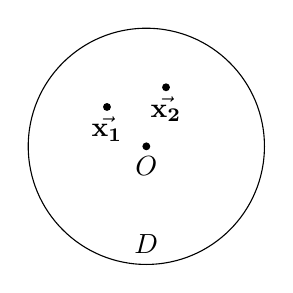
\begin{tikzpicture}
      \coordinate [label=below:$O$](O) at (0,0);
      \fill (O) circle (0.05);
      \coordinate [label=below:$\va{x_1}$](x1) at (-0.5,0.5);
      \fill (x1) circle (0.05);
      \coordinate [label=below:$\va{x_2}$](x2) at (0.25,0.75);
      \fill (x2) circle (0.05);
      \draw (0,0) circle (1.5);
      \draw (0,-1) node[below] {$D$}; %D
    \end{tikzpicture}
  \end{minipage}
  $\xrightarrow{\Phi}$
  \begin{minipage}{3cm}
    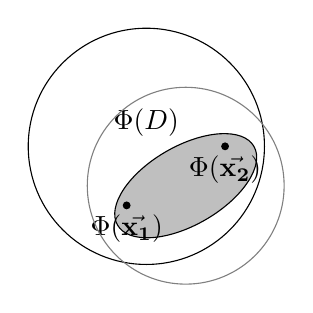
\begin{tikzpicture}
      \draw (0,0) circle (1.5);
      \coordinate [label=above:$\Phi\qty(D)$](pd) at (0,0);
      \filldraw[fill=lightgray,draw=black] (0.5,-0.5) circle [x radius=1, y radius=0.5, rotate=30];
      \coordinate [label=below:$\Phi\qty(\va{x_1})$](px1) at (-0.25,-0.75);
      \fill (px1) circle (0.05);
      \coordinate [label=below:$\Phi\qty(\va{x_2})$](px2) at (1,0);
      \fill (px2) circle (0.05);
      \draw[gray] (0.5,-0.5) circle(1.25);
    \end{tikzpicture}
  \end{minipage}
  $\xrightarrow{\Phi}$
  \begin{minipage}{3cm}
    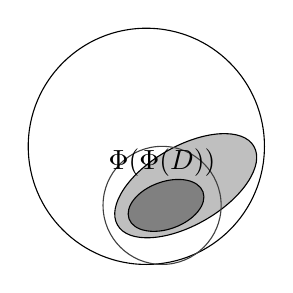
\begin{tikzpicture}
      \draw (0,0) circle (1.5);
      \filldraw[fill=lightgray,draw=black] (0.5,-0.5) circle [x radius=1, y radius=0.5, rotate=30];
      \filldraw[fill=gray,draw=black] (0.25,-0.75) circle [x radius=0.5, y radius=0.3, rotate=20];
      \draw[darkgray] (0.2,-0.75) circle(0.75);
      \coordinate [label=above:$\Phi\qty(\Phi\qty(D))$](ppd) at (0.2,-0.5);
    \end{tikzpicture}
  \end{minipage}
  $\xrightarrow{\Phi}\cdots$($\Phi\qty(D)$は半径$c\qty(<1)$のある円板に含まれる
  ($\Phi\qty(0)$からの距離$\leq c$))
  となって$c^n\xrightarrow[n\to\infty]{\ }0$なので$\Phi^n\qty(D)$は$n\to\infty$で\text{$D$内のある1点$\va{x_\infty}$に縮む}.この点$\va{x_\infty}\in D$に関しては$\Phi\qty(\va{x_\infty})=\va{x_\infty}$となるので,\\
  \underline{$\Phi:D\to D$が縮小写像なら,$\Phi$の不動点$\in D$が唯一つ存在}となる.\\
  以上のことを$\bbR^2$の代わりに\underline{関数のなす空間}に対して行いたい:\\
  \underline{設定}\quad 閉区間$I\subset\bbR$に対して
  \[C^0\qty(I,\bbR^n)=\qty{\va{x}:I\to\bbR\mid\va{x}\text{の各成分は連続関数}}\]
  とおき,(\underline{注}\,これは関数の和とスカラー倍に関して$\infty$次元のベクトル空間をなす)\\
  $\va{x}\in C^0\qty(I,\bbR)$の「長さ」(\underline{$C^0$-norm})を
  \[\norm{\va{x}}=\max_{t\in I}\abs{\va{x}\qty(t)}\]
  で定める($1\cdot 1$は$\bbR^n$での長さ)\\
  このとき\underline{$C^0\qty(I,\bbR^n)$の任意のCauthy列}($\norm{\varphi_m-\varphi_l}\xrightarrow[m,l\to\infty]{\ }0$となる$\qty{\varphi_m}\underset{m=1,2}{\subset}C^0\qty(I,\bbR^n)$)はある$\varPhi_\infty\in C^0\qty(I,\bbR^n)$に収束する(これを$C^0\qty(I,\bbR^n)$の\underline{完備性}という)
  \begin{proof}
    \begin{align*}
      \norm{\varphi_m-\varphi_l}\xrightarrow[m,l\to\infty]{\ }0
       & \Rightarrow\text{各}t\in I\text{で}\abs{\varphi_m\qty(t)-\varphi_l\qty(t)}\xrightarrow[m,l\to\infty]{\ }0                               \\
       & \Rightarrow\text{各}t\in I\text{で}\qty{\varphi_m\qty(t)}_{m=1,2}\text{はある}r_\infty\in\bbR^n\text{に収束} & \qty(C^0\text{の完備性})
    \end{align*}
    この$r_\infty$を$\varphi_\infty\qty(t)$を書くと$\varphi_m\qty(t)$は$\varphi_\infty\qty(t)$に\underline{$I$上一様収束}する($\sup_{t\in I}\abs{\varphi_m\qty(t)-\varphi_\infty\qty(t)}\xrightarrow[m\to\infty]{\ }0$となる)\\
    このとき「連続関数の一様収束極限は連続関数になる」により$\varphi_\infty$は$I$上で連続.すなわち$\varphi_\infty\in C^0\qty(I,\bbR^n)$となる.
  \end{proof}
  \subsection{$f$に課す条件(Lipschitz条件)}
  \begin{dfn*}
    $R\subset\bbR\times\bbR^n\qty(\ni\qty(t,\va{v}))$に対して$f\qty(t,\va{v})$が$R$上$\va{v}$に関して(一様)\underline{Lipschitz条件}を満たす.\\
    $\Leftrightarrow$\,ある定数$k>0$\,(Lipschitz constantという)があって各$\qty(t,\va{v_1}),\qty(t,\va{v_2})$に対して
    \[\abs{f\qty(t,\va{v_1}-f\qty(t,\va{v_2}))}\leq k\abs{\va{v_1}-\va{v_2}}\]
    を満たす(\underline{注}\,(右辺)は$t$に依らない)
  \end{dfn*}
\end{example}%
\begin{example}
  $n=1,R\subset\bbR\times\bbR$が有界閉集合で$f$が$R$上$C^1$-級\\
  $\Rightarrow$\,$t$を固定すると平均値の定理により
  \[\frac{f\qty(t,\va{v_1}-f\qty(t,\va{v_2}))}{\va{x_1}-\va{x_2}}=\pdv{f}{v}\qty(t,w)\]
  となる.点$w$が$v_1$と$v_2$の間に少なくとも1つあるので
  \[\max_{\qty(t,v)\in R}\abs{\pdv{f}{v}\qty(t,v)}=k\]
  とおくと
  \[\abs{f\qty(t,v_1)-f\qty(t,v_2)}\leq k\abs{v_1-v_2}\]
  となって$f$は$R$上$v$に関してLipschitz条件を満たす.
\end{example}
このとき
\begin{thm*}
  $R=\qty{\qty(t,\va{v})\in\bbR\times\bbR^n\mid\abs{t-t_0}\leq a,\abs{\va{v}-\va{x_0}}\leq b}$(有界閉集合)とし,
  \begin{align*}
    \begin{array}{cccc}
      f: & R                     & \to         & \bbR^n                \\
         & \rotatebox{90}{$\in$} &             & \rotatebox{90}{$\in$} \\
         & \qty(t,\va{v})        & \longmapsto & f\qty(t,\va{v})
    \end{array}
  \end{align*}
  は連続かつ$R$上$\va{v}$についてLipschitz条件を満たすとする.ここで$f\qty(t,\va{v})\leq M\quad\qty(\qty(t,\va{v})\in R)$として
  \[\alpha=\min\qty{a,\frac{b}{M}}\qty(>0)\]
  とおくと,$\qty[t_0-\alpha,t_0+\alpha]$上で定義された
  \begin{empheq}[left=\redast\empheqlbrace]{align*}
    \dv{\va{x}}{t}&=f\qty(t,\va{x}\qty(t))\\
    \va{x}\qty(t_0)&=\va{x_0}
  \end{empheq}
  の解$\va{x}=\va{x}\qty(t)$が\underline{唯一つ存在}
\end{thm*}
\begin{note}
  ($t$を$\qty[t_0-a,t_0+a]$ではなく$\qty[t_0-\alpha,t_0+\alpha]$上に制限する理由)
  \[\dv{\va{x}}{t}=f\qty(t,\va{x})\]
  より
  \[\abs{\dv{\va{x}}{t}}=\abs{f\qty(t,\va{x})}\leq M\quad\qty(\qty|\text{傾き}|\leq M)\]
  となるので
  \[\abs{\va{x}\qty(t)-\va{x}\qty(t_0)}=\abs{\int_{t_0}^t\dv{\va{x}}{s}\qty(s)\dd{s}}\leq\abs{\int_{t_0}^tM\dd{s}}=M\abs{t-t_0}\]
  となって解は
  \begin{tikzpicture}
    \draw[->] (-3.2,0)--(3.2,0)node[right]{$t$};
    \fill[lightgray] (3,3)--(3,1)--(0,2)--cycle;
    \fill[lightgray] (-3,3)--(-3,1)--(0,2)--cycle;
    \draw (-3,1)--(3,3)node[right]{傾き$M$};
    \draw (-3,3)--(3,1)node[right]{傾き$-M$};
    \draw (0,0) node[below]{$t_0$};
    \draw [dotted](0,0)--(0,2);
    \draw (0,2) node[above]{$\qty(t_0,\va{x_0})$};
  \end{tikzpicture}
  の中に入る.\\ ここで$R$の形が
  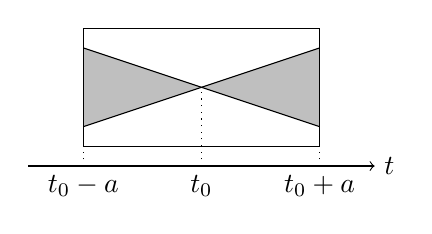
\begin{tikzpicture}
    \draw[->] (-2.2,0)--(2.2,0)node[right]{$t$};
    \fill[lightgray] (1.5,1.5)--(1.5,0.5)--(0,1)--cycle;
    \fill[lightgray] (-1.5,1.5)--(-1.5,0.5)--(0,1)--cycle;
    \draw (-1.5,0.5)--(1.5,1.5);
    \draw (-1.5,1.5)--(1.5,0.5);

    \draw (-1.5,1.75)--(-1.5,0.25)--(1.5,0.25)--(1.5,1.75)--cycle;
    \draw (0,0) node[below]{$t_0$};
    \draw [dotted](0,0)--(0,1);
    \draw (1.5,0) node[below]{$t_0+a$};
    \draw [dotted](1.5,0)--(1.5,0.25);
    \draw (-1.5,0) node[below]{$t_0-a$};
    \draw [dotted](-1.5,0)--(-1.5,0.25);
  \end{tikzpicture}
  ならよいが
  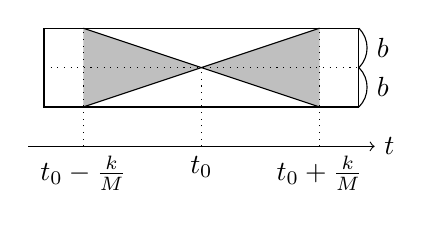
\begin{tikzpicture}
    \draw[->] (-2.2,0)--(2.2,0)node[right]{$t$};
    \fill[lightgray] (1.5,1.5)--(1.5,0.5)--(0,1)--cycle;
    \fill[lightgray] (-1.5,1.5)--(-1.5,0.5)--(0,1)--cycle;
    \draw (-1.5,0.5)--(1.5,1.5);
    \draw (-1.5,1.5)--(1.5,0.5);

    \draw (-2,1.5)--(-2,0.5)--(2,0.5)--(2,1.5)--cycle;
    \draw [dotted](-2,1)--(2,1);
    \draw (0,0) node[below]{$t_0$};
    \draw [dotted](0,0)--(0,1);
    \draw (1.5,0) node[below]{$t_0+\frac{k}{M}$};
    \draw [dotted](1.5,0)--(1.5,1.5);
    \draw (-1.5,0) node[below]{$t_0-\frac{k}{M}$};
    \draw [dotted](-1.5,0)--(-1.5,1.5);

    \draw (2,1.5) to [out=-45,in=45] node [right]{$b$} (2,1);
    \draw (2,1) to [out=-45,in=45] node[right]{$b$} (2,0.5);
  \end{tikzpicture}
  なら$t$が
  \[\abs{t-t_0}\leq\frac{b}{M}\]
  を超えると解$\va{x}\qty(t)$が$R$の外に出る可能性があり,$R$の外ではLipschitz条件が保証されないので何も言えなくなる.
\end{note}
\subsubsection{定理を示す}
\begin{proof}
  まず,十分小な$\varepsilon>0$を固定(実は$\frac{1}{2k}-\varepsilon>0$ならよい)
  \begin{align*}
    \hat{\alpha} & =\min\qty{a,\frac{b}{M},\frac{1}{2k}-\varepsilon},                                                                              & \qty(\frac{1}{2k}-\varepsilon\text{は}\Phi\text{を縮小写像にするため}) \\
    I            & =\qty[t_0-\hat{\alpha},t_0+\hat{\alpha}],                                                                                                                                                                \\
    D            & =\qty{\va{x}\in C^0\qty(I,\bbR^n)\mid\text{各}t\in I\text{に対して}\abs{\va{x}\qty(t)-\va{x_0}}\leq b}\subset C^0\qty(I,\bbR^n)
  \end{align*}
  とおき,(\underline{注}\,この$D$は$C^0\qty(I,\bbR^n)$の閉部分集合で,$D$内の点列の$\lim t\subset D$となる)
  \[\qty(\Phi\qty(\va{x}))\qty(t)=\va{x_0}+\int_{t_0}^tf\qty(s,\va{x}\qty(s))\dd{s}\]
  とする.このとき
  \begin{enumerate}
    \item[claim 1] $\Phi\qty(D)\subseteq D$
          \begin{proof}
            $\va{x}\in D,t\in I$に対して
            \begin{align*}
              \abs{\qty(\Phi\qty(\va{x}))\qty(t)-\va{x_0}}
               & =\abs{\int_{t_0}^tf\qty(s,\va{x}\qty(s))\dd{s}}          \\
               & \leq\abs{\int_{t_0}^t\abs{f\qty(s,\va{x}\qty(s))}\dd{s}} \\
               & \leq\abs{\int_{t_0}^tM\dd{s}}\tag{$\ast$}\label{20-c1}   \\\
               & \leq M\abs{t-t_0}                                        \\
               & \leq M\hat{\alpha}\leq M\frac{b}{M}=b
            \end{align*}
            ((\ref{20-c1})について\\
            $\va{x}\in D,t\in I$より
            \[\abs{s-t_0}\leq\abs{t-t_0}\Rightarrow s\in I\Rightarrow\abs{\va{x}\qty(s)-\va{x_0}}\leq b\]
            より
            \[\qty(s,\va{x}\qty(s))\in R\]
            従って
            \[\abs{f\qty(s,\va{x}\qty(s))}\leq M\])
            従って$\Phi\qty(D)\subseteq D.$
          \end{proof}
    \item[claim 2] $\Phi:D\to D$は縮小写像
          \begin{proof}
            $\va{x_1},\va{x_2}\in D$に対して
            \begin{align*}
              \norm{\Phi\qty(\va{x_1})-\Phi\qty(\va{x_2})}
               & =\max_{t\in I}\abs{\int_{t_0}^t f\qty(s,\va{x_1}\qty(s))-f\qty(s,\va{x_2}\qty(s))\dd{s}}                                                                                                 \\
               & \leq\max_{t\in I}\abs{\int_{t_0}^t\abs{f\qty(s,\va{x_1}\qty(s))-f\qty(s,\va{x_2}\qty(s))}\dd{s}}                                                                                         \\
               & \leq\max_{t\in I}\abs{\int_{t_0}^tk\abs{\va{x_1}-\va{x_2}\qty(s)}\dd{s}}                         & \qty(f\text{-Lipschitz})                                                              \\
               & \leq k\norm{\va{x_1}-\va{x_2}}\qty(I\text{の幅})                                                 & \qty(\abs{\va{x_1}-\va{x_2}\qty(s)}<\norm{\va{x_1}-\va{x_2}}\qty(s\text{によらない})) \\
               & =2k\hat{\alpha}\norm{\va{x_1}-\va{x_2}}                                                          & \qty(\qty(I\text{の幅})=2\hat{\alpha})                                                \\
               & =c\norm{\va{x_1}-\va{x_2}}                                                                       & \qty(2k\hat{\alpha}\leq 1-2k\varepsilon=c\text{とおく})
            \end{align*}
            ここで$k>0,\varepsilon>0,\frac{1}{2k}-\varepsilon>0$より$0<c<1$となるので$\Phi$は縮小写像
          \end{proof}
  \end{enumerate}
  従って$C^0\qty(I,\bbR^n)$の完備性,$D\subset C^0\qty(I,\bbR^n)$が閉部分集合により,$\Phi:D\to D$の不動点$\va{x_\infty}\in D$が唯一つ存在.
  \subparagraph{解の延長}
  \[\hat{\alpha}=\min\qty{a,\frac{b}{M},\frac{1}{2k}-\varepsilon}\lneq\min\qty{a,\frac{b}{M}}=\alpha\]
  のとき
  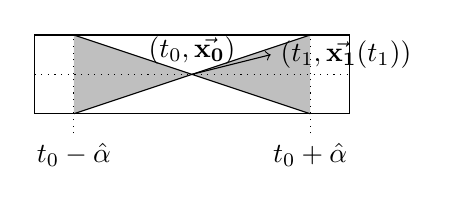
\begin{tikzpicture}
    \fill[lightgray] (1.5,1.5)--(1.5,0.5)--(0,1)--cycle;
    \fill[lightgray] (-1.5,1.5)--(-1.5,0.5)--(0,1)--cycle;
    \draw (-1.5,0.5)--(1.5,1.5);
    \draw (-1.5,1.5)--(1.5,0.5);

    \draw (-2,1.5)--(-2,0.5)--(2,0.5)--(2,1.5)--cycle;
    \draw [dotted](-2,1)--(2,1);
    \draw (0,1) node[above]{$\qty(t_0,\va{x_0})$};
    \draw (1.5,0.25) node[below]{$t_0+\hat{\alpha}$};
    \draw [dotted](1.5,0.25)--(1.5,1.5);
    \draw (-1.5,0.25) node[below]{$t_0-\hat{\alpha}$};
    \draw [dotted](-1.5,0.25)--(-1.5,1.5);

    \draw [->](0,1)--(1,1.25) node[right]{$\qty(t_1,\va{x_1}\qty(t_1))$};
  \end{tikzpicture}
  となる$\qty(t_1,\va{x_1}\qty(t_1))\quad\qty(\abs{t_1-t_0}<\frac{1}{2k}-\varepsilon)$を1つとり,この点を中心に
  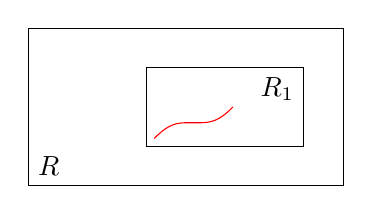
\begin{tikzpicture}
    \draw (0,0)node[above right]{$R$}--(0,2)--(4,2)--(4,0)--cycle;
    \draw (1.5,0.5)--(1.5,1.5)--(3.5,1.5)node[below left]{$R_1$}--(3.5,0.5)--cycle;
    \draw[red] (1.6,0.6)to[out=45,in=180](2,0.8)to(2.2,0.8)to[out=0,in=-135](2.6,1);
  \end{tikzpicture}
  を考えて,上と同じ議論を行うと$t_0$が$t_1$に代わった分だけ,解$\va{x}\qty(t)$の定義域が延びる.この操作を左右に有限回行うと$\frac{1}{2k}-\varepsilon$で切られた分が回復できて$\qty[t_0-\alpha,t_0+\alpha]$にまで解$\va{x}\qty(t)$が延長できる.
\end{proof}
\subsubsection{定理の適用例}
\[f\qty(t,\va{v})=A\qty(t)\va{v}+\va{b}\qty(t)\quad\qty(A\qty(t)=\qty(a_{ij}\qty(t)):n\times n\text{行列},\va{b}\qty(t)\text{の各成分が連続})\Rightarrow f\text{は}R\text{上}\va{v}\text{に関してLipschitz}\]
\begin{proof}
  $t$を固定.$A\qty(t)\in\bbC^{n^2}$と思ったときのnorm
  \[\norm{A\qty(t)}=\qty(\sum_{i,j=1}^n\abs{a_{ij}\qty(t)}^2)^\frac{1}{2}\]
  を考え,
  \[\max_{\abs{t-t_0}\leq a}\norm{A\qty(t)}=k\]
  とおくと
  \[\abs{A\qty(t)\va{v}}\leq\norm{A\qty(t)}\abs{\va{v}}\]
  なので
  \[\abs{f\qty(t,\va{v_1})-f\qty(t,\va{v_2})}=\abs{A\qty(t)\va{v_1}-A\qty(t)\va{v_2}}\leq\norm{A\qty(t)}\abs{\va{v_1}-\va{v_2}}\leq k\abs{\va{v_1}-\va{v_2}}\]
\end{proof}
従って
\begin{empheq}[left=\redast\empheqlbrace]{align*}
  \dv{\va{x}}{t}&=f\qty(t,\va{x}\qty(t))&\qty(f:\bbR\times\bbR^n\to\bbR^n)\\
  \va{x}\qty(t_0)&=\va{x_0}
\end{empheq}
の解の存在と一意性が成り立つ.
\section{ODEの解の初期値に関する連続性}
\subparagraph{主張} $f\qty(t,\va{v}):\bbR\times\bbR^n\to\bbR^n$が$R=\qty{\qty(t,\va{v})\in\bbR\times\bbR^n\mid\qty|t-t_0|\leq a,\qty|\va{v}-\va{x_0}|\leq b}$上で連続かつ$\va{v}$に関してLipschitz(ある定数$k>0$があって$\qty(t,\va{v_1}),\qty(t,\va{v_2})\in R\Rightarrow\abs{f\qty(t,\va{v_1}-f\qty(t,\va{v_2}))}\leq k\abs{\va{v_1}-\va{v_2}})$のとき
\begin{empheq}[left=\empheqlbrace]{align*}
  \dv{\va{x}}{t}&=f\qty(t,\va{x}\qty(t))\\
  \va{x}\qty(t_0)&=\va{x_0}
\end{empheq}
の(ただ一つの)解を$\va{x}\qty(t;\va{x_0})$と書くと$\va{x}\qty(t;\va{x_0})$は$\va{x_0}$に関して連続
\subparagraph{準備} \underline{Gronwallの補題}\,定数$C\geq 0,k>0$で,関数$\varphi\qty(t)$が$t_0\leq t\leq t_0+a$で連続で$\varphi\qty(t)\geq 0$となるとき,もし各$t\in\qty[t_0,t_0+a]$で
\[\varphi\qty(t)\leq C+k\int_{t_0}^t\varphi\qty(s)\dd{s}\]
を満たす.\\
$\Rightarrow$\,各$t\in\qty[t_0,t_0+a]$で
\[\varphi\qty(t)\leq Ce^{k\qty(t-t_0)}\]
が成り立つ.
\begin{proof}
  \[\Phi\qty(t)=C+k\int_{t_0}^t\varphi\qty(s)\dd{s}\]
  とおくと
  \[\Phi^\prime\qty(t)=k\varphi\qty(t)\]
  となり
  \[\Phi^\prime\qty(t)=k\varphi\qty(t)\leq k\Phi\qty(t)\]
  となる.従って
  \begin{align*}
    \dv{t}\qty(\Phi\qty(t)e^{-k\qty(t-t_0)})
     & =\Phi^\prime\qty(t)e^{-k\qty(t-t_0)}+\Phi\qty(t)\qty(e^{-k\qty(t-t_0)})^\prime & \qty(\qty(e^{-k\qty(t-t_0)})^\prime=-ke^{-k\qty(t-t_0)}) \\
     & =e^{-k\qty(t-t_0)}\qty(\Phi^\prime\qty(t)-k\Phi\qty(t))\leq 0
  \end{align*}
  となって$\Phi\qty(t)e^{-k\qty(t-t_0)}$は単調減少となる.ゆえに\[\Phi\qty(t)e^{-k\qty(t-t_0)}\leq\Phi\qty(t_0)e^{-k\qty(t_0-t_0)}=\Phi\qty(t_0)=C\]
  となって
  \[\Phi\qty(t)\leq Ce^{k\qty(t-t_0)}\]
  を得る.

  \textbf{主張}を示す.
  \begin{align*}
    \begin{cases}
      \dv{\va{x}}{t}  & =f\qty(t,\va{x}_0) \\
      \va{x}\qty(t_0) & =\va{x_0}
    \end{cases}\Leftrightarrow
    \va{x}\qty(t)-\va{x_0}=\int_{t_0}^tf\qty(s,\va{x}\qty(s))\dd{s}
  \end{align*}
  であった($\because $前章)ので初期値が$\va{x_i}$の解$\va{x}\qty(t,\va{x_i})\,\qty(i=1,2)$に対して
  \begin{align*}
    \va{x}\qty(t;\va{x_1})-\va{x}\qty(t;\va{x_2})
     & =\qty(\va{x_1}+\int_{t_0}^tf\qty(s,\va{x}\qty(s;\va{x_1}))\dd{s})-\qty(\va{x_2}+\int_{t_0}^tf\qty(s,\va{x}\qty(s;\va{x_2}))\dd{s}) \\
     & =\qty(\va{x_1}-\va{x_2})+\int_{t_0}^t\qty{f\qty(s,\va{x}\qty(s;\va{x_1}))-f\qty(s,\va{x}\qty(s;\va{x_2}))}\dd{s}
  \end{align*}
  となる.ここで\\
  \underline{$t\geq t_0$のとき}
  \begin{align*}
    \qty|\va{x}\qty(t;\va{x_1})-\va{x}\qty(t;\va{x_2})|
     & \leq\qty|\va{x_1}-\va{x_2}|+\int_{t_0}^t\qty|f\qty(s,\va{x}\qty(s;\va{x_1}))-f\qty(s,\va{x}\qty(s;\va{x_2}))|\dd{s} \\
     & =C+k\int_{t_0}^t\qty|\va{x}\qty(s;\va{x_1})-\va{x}\qty(s;\va{x_2})|\dd{s}
  \end{align*}
  ただし,$C=\qty|\va{x_1}-\va{x_2}|$とおき,解$\va{x}\qty(t,\va{x_i})$が$t_0\leq s\leq t$で$\qty(s,\va{x}\qty(s;\va{x_i}))\in R$となるような$t_0$に十分近い$t$のみ考える.
  \[\qty|f\qty(s,\va{x}\qty(s;\va{x_1}))-f\qty(s,\va{x}\qty(s;\va{x_2}))|\leq \qty|\va{x}\qty(s;\va{x_1})-\va{x}\qty(s;\va{x_2})|\]
  ここで
  \[\varphi\qty(t)=\qty|\va{x}\qty(t;\va{x_1})-\va{x}\qty(t;\va{x_2})|\]
  とおくと$\varphi\qty(t)\geq 0$でGronwallの仮定を満たすので
  \[\varphi\qty(t)\leq Ce^{k\qty(t-t_0)}\]
  \underline{$t\leq t_0$のとき}
  $s$の代わりに$\qty(-s)$を考えると,同様に
  \[\varphi\qty(t)\leq Ce^{k\qty(\qty(-t)-\qty(-t_0))}=Ce^{k\qty(t-t_0)}\]
  となる.

  これらは
  \[\qty|\va{x}\qty(t;\va{x_1})-\va{x}\qty(t;\va{x_2})|\leq\qty|\va{x_1}-\va{x_2}|e^{k\qty|t-t_0|}\]
  を意味し,各$t$で
  \[\va{x_1}-\va{x_2}\to 0\Rightarrow \va{x}\qty(t;\va{x_1})-\va{x}\qty(t;\va{x_2})\to 0\]
  が成り立ち,$\va{x}\qty(t;\va{x_0})$は$\va{x_0}$に関して連続となる.
\end{proof}
\begin{note}
  ODEの解の初期値に関する微分可能性($f\qty(t,\va{v})$が$\va{v}$に関して$C^r$-級($r\geq 1$)\,$\Rightarrow$\,解$\va{x}\qty(t;\va{x_0})$は$\va{x_0}$に関して$C^r$-級)も言える.
\end{note}

\subsection{相平面}
$n=2$の場合
\[\redast:\dv{\va{x}}{t}=A\va{x}\qty(t)\quad\qty(\va{x}\qty(t)=\mqty(
    \va{x_1}\qty(t)\\
    \va{x_2}\qty(t)),A\text{は各成分が定数の}2\times 2\text{行列})\]
の解$\va{x}\qty(t)$の軌道を$\qty(x_1,x_2)$-平面(\underline{相平面}という)上に描きたい.簡単のため\underline{仮定}$A$の2つの固有値$\lambda_1,\lambda_2$は共に$\neq 0$とする.(→\redast の解$\va{x}\qty(t)=\va{0}$の近くには動かない解軌道はない)\\
$A$はある$2\times 2$正則行列$P=\mqty(\va{p_1}&\va{p_2})$によって
\[P^{-1}AP=\begin{cases}
    \mqty(
    \lambda_1 & 0                 \\
    0         & \lambda_2
    )\to\text{\underline{Case 1}} \\
    \mqty(
    \lambda_1 & 1                 \\
    0         & \lambda_1
    )\to\text{\underline{Case 2}}
  \end{cases}\]
と出来た.この$P$を使って
\[P^{-1}\va{x}\qty(t)=\va{X}\qty(t)=\mqty(X_1\qty(t)\\X_2\qty(t))\]
とおくと
\[\va{x}\qty(t)=P\va{X}\qty(t)\]
より
\[\dv{\va{x}}{t}=A\va{x}\Leftrightarrow P\dv{\va{X}}{t}=AP\va{X}\Leftrightarrow\dv{\va{X}}{t}=P^{-1}AP\va{X}\]
となる.
\begin{note}
  \begin{align*}
    \va{x}\qty(t)
     & =\mqty(\va{e_1}                        & \va{e_2})\mqty(x_1\qty(t) \\x_2\qty(t))\\
     & =P\va{X}\qty(t)=\mqty(\va{p_1}         & \va{p_2})\mqty(X_1\qty(t) \\X_2\qty(t))\\
     & =X_1\qty(t)\va{P_1}+X_2\qty(t)\va{p_2}
  \end{align*}
  となって$\va{p_1}$方向が$X_1$軸方向となる.
\end{note}
\subparagraph{Case 1のとき}
\[\dv{t}\mqty(X_1\\X_2)=\mqty(\lambda_1X_1\\\lambda_2X_2)\]
より,
\[\va{X}\qty(t)=\mqty(C_1e^{\lambda_1t}\\C_2e^{\lambda_2t})\quad\qty(C_1,C_2\text{は任意定数})\]
となるので解軌道$\qty{\va{x}\qty(t)\mid t\in\bbR}$は
\begin{enumerate}
  \item $\lambda_1,\lambda_2\in\bbR$で
        \begin{enumerate}
          \item $\lambda_1,\lambda_2<0$のとき
                \begin{figure}[h]
                  \begin{minipage}{0.45\textwidth}
                    \centering
                    \begin{tikzpicture}
                      \begin{scope}
                        \draw (0,0) node[below] {\scriptsize O};
                        \fill (0,0) circle (0.05);
                        \draw[->] (2,0) -- (0.3,0);
                        \draw[->] (-2,0) -- (-0.3,0);
                        \draw[->] (0,2) -- (0,0.3);
                        \draw[->] (0,-2) -- (0,-0.3);
                        \draw[->] (1.4,1.4) -- (0.2,0.2);
                        \draw[->] (1.4,-1.4) -- (0.2,-0.2);
                        \draw[->] (-1.4,1.4) -- (-0.2,0.2);
                        \draw[->] (-1.4,-1.4) -- (-0.2,-0.2);
                      \end{scope}
                    \end{tikzpicture}
                    \caption{$\lambda_1=\lambda_2$のとき}
                  \end{minipage}
                  or
                  \begin{minipage}{0.45\textwidth}
                    \centering
                    \begin{tikzpicture}
                      \draw (0,0) node[below] {\scriptsize O};
                      \fill (0,0) circle (0.05);
                      \draw[->] (2,0) node[right] {$\va{p_1}$方向} -- (0.3,0);
                      \draw[->] (-2,0) -- (-0.3,0);
                      \draw[->] (0,2) node[above] {$\va{p_2}$方向} -- (0,0.3);
                      \draw[->] (0,-2) -- (0,-0.3);
                      \begin{scope}
                        \clip (0.3, -2) rectangle (2, 2);
                        \draw plot (\x, {exp(\x -2)});
                        \draw[->] (0.4,{exp(-1.7)+0.01}) -- (0.3, {exp(-1.7)});
                        \draw plot (\x, {-exp(\x -2)});
                        \draw[->] (0.4,{-exp(-1.7)-0.01}) -- (0.3, {-exp(-1.7)});
                      \end{scope}
                      \begin{scope}
                        \clip (-2, -2) rectangle (-0.3, 2);
                        \draw plot (\x, {exp(-\x - 2)});
                        \draw[->] (-0.4,{exp(-1.7)+0.01}) -- (-0.3, {exp(-1.7)});
                        \draw plot (\x, {-exp(-\x - 2)});
                        \draw[->] (-0.4,{-exp(-1.7)-0.01}) -- (-0.3, {-exp(-1.7)});
                      \end{scope}
                    \end{tikzpicture}
                    \caption{$\qty|\lambda_1|<\qty|\lambda_2|$のとき}
                  \end{minipage}
                \end{figure}

                $\qty|\lambda_1|<\qty|\lambda_2|$のとき,$t\to\infty$で$e^{\lambda_1t}$より$e^{\lambda_2t}$の方が速く0に近づく.
          \item $\lambda_1,\lambda_2>0$のとき
                \begin{figure}[h]
                  \begin{minipage}{0.45\textwidth}
                    \centering
                    \begin{tikzpicture}
                      \begin{scope}
                        \draw (0,0) node[below] {\scriptsize O};
                        \fill (0,0) circle (0.05);
                        \draw[->] (0.3,0) -- (2,0);
                        \draw[->] (-0.3,0) -- (-2,0);
                        \draw[->] (0,0.3) -- (0,2);
                        \draw[->] (0,-0.3) -- (0,-2);
                        \draw[->] (0.2,0.2) -- (1.4,1.4);
                        \draw[->] (0.2,-0.2) -- (1.4,-1.4);
                        \draw[->] (-0.2,0.2) -- (-1.4,1.4);
                        \draw[->] (-0.2,-0.2) -- (-1.4,-1.4);
                      \end{scope}
                    \end{tikzpicture}
                    \caption{$\lambda_1=\lambda_2$のとき}
                  \end{minipage}
                  or
                  \begin{minipage}{0.45\textwidth}
                    \centering
                    \begin{tikzpicture}
                      \draw (0,0) node[below] {\scriptsize O};
                      \fill (0,0) circle (0.05);
                      \draw[->] (0.3,0) -- (2,0) node[right] {$\va{p_1}$方向};
                      \draw[->] (-0.3,0) -- (-2,0);
                      \draw[->] (0,0.3) -- (0,2) node[above] {$\va{p_2}$方向};
                      \draw[->] (0,-0.3) -- (0,-2);
                      \begin{scope}
                        \clip (0.3, -2) rectangle (2, 2);
                        \draw plot (\x, {exp(\x -2)});
                        \draw[->] (1.99, {exp(-0.01)}) -- (2, 1);
                        \draw plot (\x, {-exp(\x -2)});
                        \draw[->] (1.99,{-exp(-0.01)}) -- (2, -1);
                      \end{scope}
                      \begin{scope}
                        \clip (-2, -2) rectangle (-0.3, 2);
                        \draw plot (\x, {exp(-\x - 2)});
                        \draw[->] (-1.99, {exp(-0.01)}) -- (-2, 1);
                        \draw plot (\x, {-exp(-\x - 2)});
                        \draw[->] (-1.99,{-exp(-0.01)}) -- (-2, -1);
                      \end{scope}
                    \end{tikzpicture}
                    \caption{$\lambda_1<\lambda_2$のとき}
                  \end{minipage}
                \end{figure}

                $\qty|\lambda_1|<\qty|\lambda_2|$のとき,$t\to-\infty$で$e^{\lambda_1t}\gg e^{\lambda_2t}$
          \item $\lambda_1,\lambda_2$が異符号($\lambda_1<0<\lambda_2$とする)とき
          \begin{figure}[h]
            \begin{minipage}{0.45\textwidth}
              \centering
              \begin{tikzpicture}
                \draw (0,0) node[below] {\scriptsize O};
                \fill (0,0) circle (0.05);
                \draw[->] (2,0) node[right] {$\va{p_1}$方向} -- (0.3,0);
                \draw[->] (-2,0) -- (-0.3,0);
                \draw[->] (0,0.3) -- (0,2) node[above] {$\va{p_2}$方向};
                \draw[->] (0,-0.3) -- (0,-2);
                \draw[<-] (0.25, 2) .. controls (0.5, 0.5) .. (2, 0.25);
                \draw[<-] (0.25, -2) .. controls (0.5, -0.5) .. (2, -0.25);
                \draw[<-] (-0.25, 2) .. controls (-0.5, 0.5) .. (-2, 0.25);
                \draw[<-] (-0.25, -2) .. controls (-0.5, -0.5) .. (-2, -0.25);
              \end{tikzpicture}
            \end{minipage}
          \end{figure}
        \end{enumerate}

  \item $\lambda_1,\lambda_2\not\in\bbR$で
  \begin{empheq}[left=\empheqlbrace]{align*}
    \lambda_1&=p+iq\\
    \lambda_2&=p-iq
  \end{empheq}
  ただし$p,q\in\bbR,q=\neq 0$のとき
  \[\mqty(X_1\qty(t)\\X_2\qty(t))=\mqty(C_1e^{\lambda_1t}\\C_2e^{\lambda_2t})\in\bbC^2\]
  に対して
  \begin{empheq}[left=\empheqlbrace]{align*}
    Z_1\qty(t)&=\frac{X_1\qty(t)+X_2\qty(t)}{2}\\
    Z_2\qty(t)&=\frac{X_1\qty(t)-X_2\qty(t)}{2i}
  \end{empheq}
  とおくと
  \begin{align*}
    Z_1\qty(t)&=\frac{1}{2}e^{pt}\qty(C_1e^{iqt}+C_2e^{-iqt})=e^{pt}\qty{\frac{C_1+C_2}{2}\cos\qty(qt)+\frac{iC_1-iC_2}{2}\sin\qty(qt)}\\
    Z_2\qty(t)&=e^{pt}\qty{\frac{C_1+C_2}{2}\sin\qty(qt)+\frac{C_1-C_2}{2i}\cos\qty(qt)}
  \end{align*}
  $\tilde{C_1}=\frac{C_1+C_2}{2},\tilde{C_2}=\frac{iC_1-iC_2}{2}$とおく.ここで$\tilde{C_1},\tilde{C_2}$を$\bbR$に制限すると$\bbR^2$上の解軌道として
  \begin{empheq}[left=\empheqlbrace]{align*}
    Z_1\qty(t)
    &=e^{pt}\qty{\tilde{C_1}\cos\qty(qt)+\tilde{C_2}\sin\qty(qt)}\\
    &=\sqrt{\tilde{C_1}^2+\tilde{C_2}^2}e^{pt}\qty{\cos\qty(qt)\frac{\tilde{C_1}}{\sqrt{\tilde{C_1}^2+\tilde{C_2}^2}}+\sin\qty(qt)\frac{\tilde{C_2}}{\sqrt{\tilde{C_1}^2+\tilde{C_2}^2}}}\\
    &=Ce^{pt}\cos\qty(qt-\alpha)\quad\qty(C=\sqrt{\tilde{C_1}^2+\tilde{C_2}^2}\text{とおく})\\
    Z_2\qty(t)
    &=e^{pt}\qty{\tilde{C_1}\sin\qty(qt)-\tilde{C_2}\cos\qty(qt)}\\
    &=\sqrt{\tilde{C_1}^2+\tilde{C_2}^2}e^{pt}\qty{\sin\qty(qt)\frac{\tilde{C_1}}{\sqrt{\tilde{C_1}^2+\tilde{C_2}^2}}-\cos\qty(qt)\frac{\tilde{C_2}}{\sqrt{\tilde{C_1}^2+\tilde{C_2}^2}}}\\
    &=Ce^{pt}\sin\qty(qt-\alpha)
  \end{empheq}
  となるので
\end{enumerate}

\newpage
\section*{レポート課題}
\subsection*{問1}
$x=x\qty(t)$に対するODE
\[\dv{x}{t}=\qty(\frac{x}{t})^2+\frac{x}{t}+1\]
を同次型の解法で解け.
\subsection*{問2}
$x=x\qty(t)$に対する
\[\dv{x}{t}+2tx=te^{t^2-t}x^2\]
をBernoulli型の解法で解け.
\subsection*{問3}
$A=\mqty(-1 & 6 \\ 2 & -2)$を対角化し,それを利用して$\va{x}\qty(t)=\mqty(x_1\qty(t)\\x_2\qty(t))$に対する
\[\dv{\va{x}}{t}=A\va{x}\]
を解け.
\subsection*{問4}
\[\redast:\qty(2tx^2+3t^2x^3)\dd{t}+\qty(3+4t^2x+5t^3x^2)\dd{t}=0\]
に対して,
\begin{enumerate}
  \item \redast は全微分型でないを示せ.
  \item \redast の積分因子を1つ求めて\redast の一般解$x\qty(t)$を与えよ.
\end{enumerate}
\subsection*{問5}
$D=\dv{t}$に対して
\[D^2\qty(D-1)^3\qty(D^2+2D+10)^2x=0\]
の一般解$x\qty(t)$を実数値関数で与えよ.
\subsection*{問6}
\[\qty(D^2+9)=2\cos\qty(3t)-\sin\qty(3t)\]
の一般解を与えよ.
\subsection*{問7}
\[\qty(D^2+1)x=\frac{1}{\qty(\cos t)^3}\]
の一般解を定数変化法で求めよ.
\subsection*{問8}
$A=\mqty(1&2\\-8&-7)$に対して
\begin{enumerate}
  \item $A$をJordan標準形に直し,それを利用して$e^{At}$を求めよ.
  \item $e^{At}$を射影行列の方法で求め(\underline{注}\,射影行列は$I$になる),
        \begin{empheq}[left=\empheqlbrace]{align*}
          \dv{\va{x}}{t}&=A\va{x}\\
          \va{x}\qty(0)&=\mqty(-1&1)
        \end{empheq}
        の解$\va{x}\qty(t)=\mqty(x_1\qty(t)\\x_2\qty(t))$を求めよ.
\end{enumerate}
\end{document}
